% ------------------------------------------------------------------------------
% OpenQuake-engine Users Manual
% 
% Authors: 
% 	H. Crowley 		- Executive Committee - GEM Foundation, Pavia, Italy
% 	D. Monelli 		- GEM Model Facility, Zurich, Switzerland
% 	M. Pagani 		- Executive Committee - GEM Foundation, Pavia, Italy
% 	V. Silva 		- GEM Model Facility, Pavia, Italy
%	G. Weatherhill 	- GEM Model Facility, Pavia, Italy
% 
% Document distributed under the Common Creative License 
% © GEM Foundation, Pavia, February 2013
% ------------------------------------------------------------------------------
\documentclass[12pt,a4paper,headings=small,version=last,dvips]{scrbook}
%\documentclass[12pt,a4paper,headings=small,version=first,dvips]{scrbook}
% --------------------------------------------------------------------- Packages
\setcounter{secnumdepth}{3}
\setcounter{tocdepth}{3}
% This is used to create the cover and to plot trees
\usepackage{pst-tree}
\usepackage{pstricks,pstricks-add,multido}
%
\usepackage{geometry}
\usepackage{moresize}

\usepackage{chappg}

%
%\usepackage{algorithmic}
% 
\usepackage{fancyvrb}
\usepackage{listings}
\usepackage{alltt}
\usepackage{gensymb}
%
\usepackage[section]{placeins}
% 
\usepackage{pbox}
% http://en.wikibooks.org/wiki/LaTeX/Indexing
\usepackage{makeidx} 
\makeindex
%
%\usepackage{subfigure}
% Figure caption settings
\usepackage[textfont=it,margin=10pt,font=small,labelfont=bf,labelsep=endash]{caption}
\usepackage{subcaption}
%
\usepackage{bm}
% Landscape package
\usepackage{lscape}
%
\usepackage{hyperref} 
\hypersetup{colorlinks=true}
\hypersetup{breaklinks=true}
% package for multiline comments
\usepackage{verbatim}

\usepackage{xcolor}
\usepackage{framed}
\usepackage[utf8]{inputenc}

%
% Package to create a glossary - It must be uploaded after hyperref
% to produce the glossary: makeglossaries OQB
%\usepackage[toc,acronym,nonumberlist,style=altlist]{glossaries}
\usepackage[toc,nonumberlist,style=altlist]{glossaries}
\glstoctrue
\makeglossaries
%
% - - - - - - - - - - - - - - - - - - - - - - - - - - - - - - - - Setting Fonts
% \renewcommand{\encodingdefault}{OT1}
\renewcommand{\encodingdefault}{OT1}
\renewcommand{\familydefault}{ppl}
% \renewcommand{\familydefault}{cmss}
% \renewcommand{\seriesdefault}{m}
% \renewcommand{\shapedefault}{up}

% - - - - - - - - - - - - - - - - - - - - - - - - - - - - - - - - - - - - - - -
\usepackage{amsmath}
% - - - - - - - - - - - - - - - - - - - - - - - - - - - - - - - - - - - - - - -
\usepackage{titlesec}
\usepackage[dvips]{graphicx}
% - - - - - - - - - - - - - - - - - - - - - - - - - - - - - - - - - - - - - - -
\usepackage{type1cm,eso-pic,color}

%\makeatletter
%\AddToShipoutPicture{
%    \setlength{\@tempdimb}{.5\paperwidth}
%    \setlength{\@tempdimc}{.5\paperheight}
%    \setlength{\unitlength}{1pt}
%    \put(\strip@pt\@tempdimb,\strip@pt\@tempdimc){
%        \makebox(0,0){\rotatebox{55}{
%        	\textcolor[gray]{0.85}{
%        		\fontsize{5cm}{5cm}
%        		\selectfont{DRAFT}}
%        	}
%        }
%	}
%}
%\makeatother

%
% Solves problems with margin notes
\usepackage{mparhack} 
	\setlength{\marginparwidth}{1.1in}
	\let\oldmarginpar\marginpar
	\renewcommand\marginpar[1]{\-\oldmarginpar[\raggedright\color{red01}
	\footnotesize #1]%
	{\raggedright\footnotesize #1}}
% Define some colors
	\definecolor{azure}{RGB}{240,255,255}
	\definecolor{honeydew}{RGB}{240,255,240}
	\definecolor{blue01}{RGB}{4,64,116}
	\definecolor{blue02}{RGB}{0,62,113}
	\definecolor{gray01}{rgb}{0.1,0.1,0.1}
	\definecolor{gray02}{rgb}{0.8,0.8,0.8}
	\definecolor{red01}{rgb}{0.5,0.0,0.0}
	\definecolor{orange00}{rgb}{1.0,0.74,0.53}
	\definecolor{orange01}{rgb}{0.9137,0.5882,0.0980}
	\definecolor{orange02}{rgb}{0.7608,0.4157,0.1804}
	\definecolor{orange03}{rgb}{0.6941,0.1843,0.1333}
\usepackage[english]{babel}
% Bibliography settings
\usepackage[square,colon]{natbib} % Extend bibligraphy functions
% Page numbering by Chapter
%\usepackage[auto]{chappg} 
%\pagenumbering{bychapter}
% 
% Define page properties
\usepackage{scrpage2}
	\pagestyle{scrheadings}
	\lofoot[]{}
	\refoot[]{}
	%\lofoot[]{\includegraphics[width=1.0cm]{./figures/openquake_logo.eps}}
	%\refoot[]{\includegraphics[width=1.0cm]{./figures/openquake_logo.eps}}
	%\renewcommand{\partpagestyle}{empty}
% - - - - - - - - - - - - - - - - - - - - - - - - - -  Reformatting PART Titles
\titleformat{\part}[display]
{\filleft\normalfont\sffamily}
{\textcolor{blue01}{\bfseries\large PART}\hspace{4pt}
	\bfseries\Huge\textcolor{blue01}{\thepart}}
{1pc}
{\Huge\bfseries\textcolor{blue01}}
[]
% - - - - - - - - - - - - - - - - - - - - - - - - - Reformatting CHAPTER Titles
% Titles: CHAPTER
\titleformat{\chapter}
	[display] % shape
	{\filleft\normalfont\sffamily} % format
	{\textcolor{blue01}{\bfseries\MakeUppercase{\chaptertitlename}} % label
	\hspace{4pt}\huge\bfseries\textcolor{blue01}{\thechapter}} 
	{1pc} % sep
	{\huge\bfseries\textcolor{blue01}} % Before
	[]
% - - - - - - - - - - - - - - - - - - - - - - - - - Reformatting SECTION Titles
% Titles: SECTION
\titleformat{\section}
	[hang] % shape
	{\vspace{.8ex}\Large\bfseries\color{blue01}} % format 
	{\textcolor{blue01}{\thesection.}} % label
	{.5em} % sep
	{} % before
	[] % after
% - - - - - - - - - - - - - - - - - - - - - - -  Reformatting SUBSECTION Titles
% Title: SUBSECTION
\titleformat{\subsection}
	[hang] % shape
	{\vspace{.8ex}\large\bfseries\color{blue01}} % format 
	{\textcolor{blue01}{\thesubsection.}} % label
	{.5em} % sep
	{} % before
	[] % after
%  - - - - - - - - - - - - - - - - - - - - -  Reformatting SUBSUBSECTION Titles 
% Title: SUBSUBSECTION
\titleformat{\subsubsection}
	[hang] % shape
	{\vspace{.8ex}\normalfont\bfseries\color{blue01}} % format 
	{\textcolor{blue01}{\thesubsubsection.}} % label
	{.5em} % sep
	{} % before
	[] % after
% - - - - - - - - - - - - - - - - - - - - - - -  Reformatting PARAGRAPH Titles 
% Title: PARAGRAPH
\titleformat{\paragraph}
	[hang] % shape
	{\vspace{.2ex}\normalfont\color{blue01}} % format 
	{} % label
	{} % sep
	{} % before
	[] % after
%

% ------------------------------------------------------------------------------
\uppertitleback{
   \textbf{Authors:} \\
   Helen Crowley$^1$, Damiano Monelli$^2$, 
   Marco Pagani$^1$, Vitor Silva$^3$, Graeme Weatherill$^3$ \\ \hfill \\
   \small
   \begin{tabular}{p{4cm}p{4cm}p{4cm}}
   $^1$ GEM Foundation \hfill \newline
   via Ferrata, 1 \hfill \newline 
   20133 Pavia \hfill \newline
   Italy \hfill \newline
   & 
   $^2$ GEM Model Facility \hfill \newline
   SED - ETHZ \hfill \newline  
   Sonneggstrasse, 5 \hfill \newline
   CH-8092 Zurich\hfill \newline
   Switzerland \hfill \newline
   &
   $^3$ GEM Model Facility \hfill \newline 
   via Ferrata, 1 \hfill \newline 
   20133 Pavia \hfill \newline
   Italy \hfill \newline   
	\end{tabular} \hfill \newline
   %
	Email address (for all the authors):\hfill\\
   $<$name.surname$>$@globalquakemodel.org
   %
   \vspace{0.4cm} \hfill \\
   {\bf{Disclaimer}} \hfill \\
   The OpenQuake User Manual is distributed in the hope that it will be useful, 
   but without any warranty: without even the implied warranty of 
   merchantability or fitness for a particular purpose. While every 
   precaution has been taken in the preparation of this document, in 
   no event shall the authors of the manual and the GEM Foundation be 
   liable to any party for direct, indirect, special, incidental, or 
   consequential damages, including lost profits, arising out of the 
   use of information contained in this document or from the use of 
   programs and source code that may accompany it, even if the authors 
   and GEM Foundation have been advised of the possibility of such damage. 
   The Manual provided hereunder is on as "as is" basis, and the authors 
   and GEM Foundation have no obligations to provide maintenance, support,
   updates, enhancements, or modifications. 
   \hfill \\
   The current version of the manual has been revised only by members of 
   the GEM model facility and it must be considered a draft copy. 
   %
   \vspace{0.4cm} \hfill \\
   {\bf{License}} \hfill \\
   This Manual is distributed under the Creative Common License 
   Attribution-NonCommercial-NoDerivs 3.0 Unported (CC BY-NC-ND 3.0) (see link below). 
   You can download this Book and share it with others as long as you provide proper 
   credit, but you cannot change it in any way or use it commercially 
   \hfill \\
   \href{http://creativecommons.org/licenses/by-nc-nd/3.0/}
   {http://creativecommons.org/licenses/by-nc-nd/3.0/}  
   \normalsize
}  
%
% =============================================================== BEGIN DOCUMENT
% -------------------------------------------------- Title and table of contents
\begin{document}
% - - - - - - - - - - - - - - - - - - - - - - - - - - - - - -  Load the glossary
% OpenQuake Book Glossary
% To cite a glossary element in a document:
%\gls{seismicsourcedata}
%\Gls{seismicsourcedata} - First initial is uppercase
%\GLS{seismicsourcedata} - All initials are uppercase
%\glspl{seismicsourcedata} - Plural
% To process the glossary:
% makeglossaries oq-manual


% ------- A

\newglossaryentry{areasource}{
	name=area source,
	description={A source type usually adopted to model distributed
	seismicity. In an area source the seismicity occurrence rate is assumed
	uniform over the source area; this produces an hazard pattern with a
	plateau of constant hazard inside the polygon delimiting the area source
	and values of hazard that tend to decrease as we move away from the
	border of the source}
}


\newglossaryentry{asset}{
	name=asset,
	description={An asset is an element with a certain value, which can include
	buildings or population. For example, an asset can include an individual
	building at a given location, or a number of buildings that are grouped, co-
	located at a single location and classified with the same \gls{taxonomy}}
}



% ------- B

\newglossaryentry{branch}{
	name=branch,
	plural=branches,
	description={The simplest element in a logic tree; it belongs to a
	\gls{branchset} where it represents one possible option among a finite
	number of alternatives. A branch is associated with a weight value
	\citep{scherbaum2011} if the \gls{branchset} represents the epistemic
	uncertainty on a parameter or a model when the \gls{branchset} is used to
	specify alternative models (e.g. district \glspl{acr:mfd})}
}


\newglossaryentry{branchinglevel}{
	name=branching level,
	description={It indicates the position where a \gls{branchset} or a
	\gls{branch} is located in a logic tree structure. For example, the first
	branching level of the \gls{seismicsourcelogictree} always contains one
	or several \glspl{initialseismicsourceinputmodel}}
}


\newglossaryentry{branchset}{
	name=branch set,
	description={The structure describing the epistemic uncertainty on a
	specific parameter or model included in a logic tree structure. It
	ensembles a number of \glspl{branch}, each one representing a discrete
	alternative}
}



% ------- C

\newacronym{cpsha}{cPSHA}{Classical PSHA}


\newglossaryentry{configurationfile}{
	name=configuration file,
	description={Usually the file containing the information necessary to
	run a calculation in OpenQuake}
}


\newglossaryentry{consequence function}{
	name=consequence function,
	description={the distribution of the consequence (or loss) ratio conditional
	on a set of discrete limit states, defined for a particular \gls{taxonomy}}
}


\newglossaryentry{consequence model}{
	name=consequence model,
	description={A set of \glspl{consequence function} used to model the
	consequence ratios of all the \glspl{taxonomy} in the \gls{exposure model}}
}


\newglossaryentry{charfaultsource}{
	name=characteristic fault source,
	description={A fault source typology where ruptures always cover the entire
	fault surface}
}


\newglossaryentry{complexfaultsource}{
	name=complex fault source,
	description={A source typology usually adopted to model subduction
	interface faults}
}



% ------- D

\newglossaryentry{deductible}{
	name=deductible,
	description={A parameter used in the calculation of insured losses that
	establishes the economic value that needs to be deducted from the ground-up
	losses}
}


\newglossaryentry{seismichazarddisaggregation}{
	name=seismic hazard disaggregation,
	description={A methodology to investigate the contributions to a
	specific level of hazard in terms of fundamental variables commonly used
	to characterize seismic sources and ground motion models (e.g. magnitude,
	source-site distance, \gls{epsilon}}
}


\newglossaryentry{dip}{
	name=dip,
	description={The dip is the steepest angle of descent of the fault plane
	relative to a horizontal plane; it is measured in degrees [0,90]}
}


\newglossaryentry{disaggregationmatrix}{
	name=disaggregation matrix,
	description={A multi-dimensional matrix used to systematically store the
	contributions to a level of hazard to be disaggregated and that is specified
	by the user. See also \gls{seismichazarddisaggregation}}
}



% ------- E

\newacronym{acr:erf}{ERF}{Earthquake\- Rupture\- Forecast}
\newacronym{acr:epsha}{ePSHA}{Event-based PSHA}


\newglossaryentry{earthquakeruptureforecast}{
	name=earthquake rupture forecast,
	description={A list of all possible ruptures generated by all the
	sources included in a seismic source model. Each element in the list
	contains: the rupture geometry and the rupture probability of occurrence
	in a given time span. See also the definition available on the
	\href{http://www.opensha.org/glossary-earthquakeRuptureForecast} {OpenSHA
	website}}
}


\newglossaryentry{earthquakeruptureforecastcalculator}{
	name=earthquake rupture forecast calculator,
	description={Calculator producing a \gls{seismicsourcemodel} from a
	\gls{seismicsourcelogictree}}
}


\newglossaryentry{epsilon}{
	name=epsilon,
	description={normalized residual of the ground motion}
}


\newglossaryentry{exposure model}{
	name=exposure model,
	description={A set of \glspl{asset} grouped according to their
	geographical location, \gls{taxonomy} and value}
}



% ------- F

\newglossaryentry{faulttrace}{
	name=fault trace,
	description={A curve representing the intersection between the surface
	containing the fault surface (or its prolongation) and the topographic
	surface
	\begin{figure}[!ht] \centering
	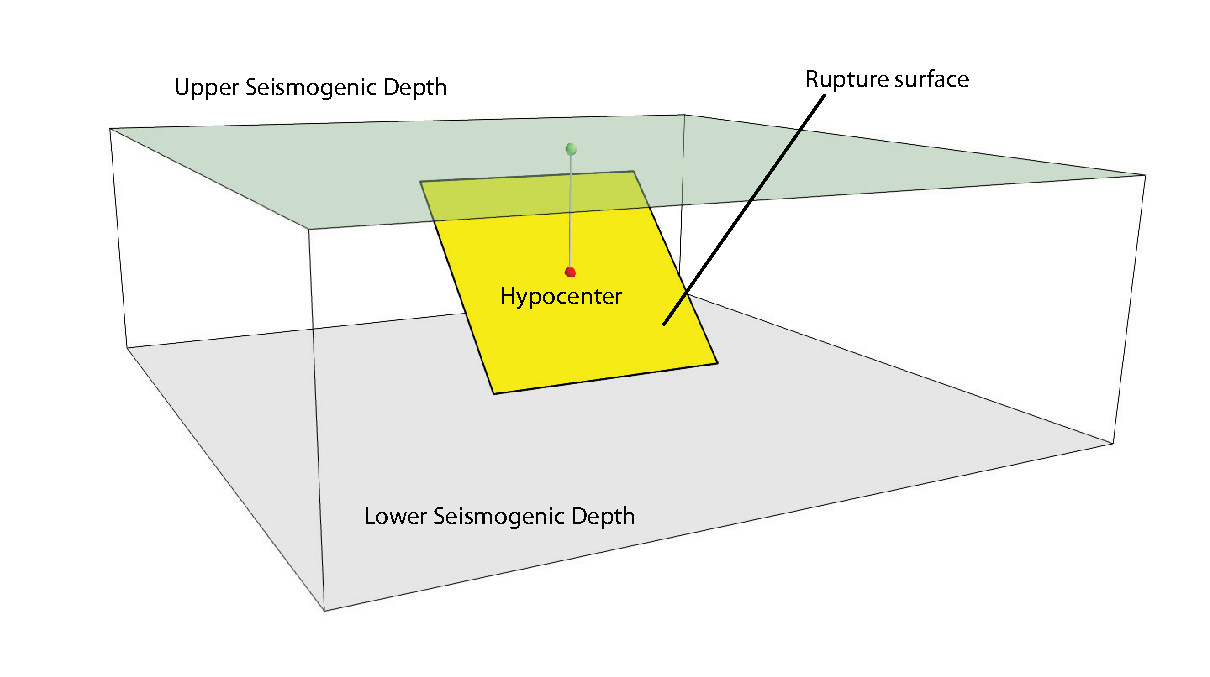
\includegraphics[width=10cm]{figures/hazard/single_rupture.pdf}
	\end{figure}}
}


\newglossaryentry{fragility function}{
	name=fragility function,
	description={the probability of exceeding a set of limit states, given
	an intensity measure level. These functions can be discrete or continuous}
}


\newglossaryentry{fragility model}{
	name=fragility model,
	description={A set of \glspl{fragility function} used to model the
	fragility of all the \glspl{asset} in the \gls{exposure model}}
}


\newglossaryentry{frequencymagnitudedistribution}{
	name=frequency-magnitude distribution,
	description={See \gls{mfd}}
}



% ------- G

\newacronym{acr:gem}{GEM}{Global Earthquake Model}
\newacronym{acr:gmf}{GMF}{Ground Motion Field}
\newacronym{acr:gmpe}{GMPE}{Ground Motion Prediction Equation}
\newacronym{acr:gmlt}{GMLT}{Ground Motion Logic Tree (see \gls{groundmotionlogictree}}


\newglossaryentry{gridsource}{
	name=grid source,
	description={A source typology usually adopted to model distributed
	seismicity. It is routinely produced by a seismicity smoothing algorithm (one
	of the most famous algorithm is the one proposed by \citet{frankel1995})}
}


\newglossaryentry{groundmotionfield}{
	name=ground-motion field,
	description={An object describing the geographic distribution around a
	rupture of a ground motion intensity measure}
}


\newglossaryentry{groundmotionfieldcalc}{
	name=ground-motion field calculator,
	description={An \gls{acr:oqe} calculator that given a rupture computes the
	geographic distribution of a ground motion intensity parameter. Currently
	OQ can generate ground motion fields using a \gls{acr:gmpe}}
}


\newglossaryentry{groundmotionlogictree}{
	name=ground-motion logic tree,
	description={A method used to systematically describe the epistemic
	uncertainties related to the ground motion models used in the computation
	of hazard using a specific \gls{pshainputmodel}}
}


\newglossaryentry{groundmotionmodel}{
	name=ground-motion model,
	description={An object that given a rupture with specific properties
	computes the expected ground motion at the given site. In simplest case a
	ground motion model corresponds to a \gls{groundmotionpredictioneq}. In
	case of complex PSHA input models, the produced ground motion models
	contains a set of \glspl{acr:gmpe}, one for each tectonic region considered}
}


\newglossaryentry{groundmotionparameter}{
	name=ground-motion parameter,
	description={A scalar or vector quantity describing a relevant property
	of the shaking such as intensity (e.g. PGA or Spectral Acceleration)
	or duration, equivalent number of cycles  \citep[see for
	example][]{hancock2005})}
}


\newglossaryentry{groundmotionpredictioneq}{
	name=ground-motion prediction equation,
	description={An equation that - given some fundamental parameters
	characterizing  the source, the propagation path and the site (in the
	simplest  case magnitude, distance and V$_\text{S,30}$) - computes the
	value $GM$ of a (scalar) ground motion intensity parameter}
}


\newglossaryentry{groundmotionsystem}{
	name=ground-motion system,
	description={An object containing a list of \gls{groundmotionlogictree}}
}



% ------- I

\newglossaryentry{initialseismicsourceinputmodel}{
	name=initial seismic source input model,
	description={It is the ensable of information needed to fully describe
	the seismic sources composing a seismic source input model. The
	initial seismic source input model is included in the first  branching
	level of a seismic source logic tree}
}


\newglossaryentry{insured losses}{
	name=insured losses,
	description={Fraction of the ground-up losses that can be covered by the
	insurance industry, according to a certain policy}
}


\newglossaryentry{investigationtime}{
	name=investigation time,
	description={The time interval considered to calculate hazard; usually
	it corresponds to 50 years}
}



% ------- L

\newglossaryentry{limit}{
	name=limit,
	description={A parameter used in the calculation of insured losses that
	establishes the maximum economic amount that can be covered by the insurance
	industry, according to a certain insurance policy}
}


\newglossaryentry{logictree}{
	name=logic tree,
	description={Data structure used to systematically describe uncertainties
	on parameters and models used in a PSHA study}
}


\newglossaryentry{logictreeprocessor}{
	name=logic tree processor,
	description={An OQ calculator that takes the PSHA Input Model and creates
	many realisations of a \gls{seismicsourcemodel} and of a
	\gls{groundmotionmodel}}
}


\newacronym{acr:ltmcs}{LTMCS}{Logic Tree Monte Carlo Sampler}


\newglossaryentry{msr}{
	name=magnitude-scaling relationship,
	description={An empirical relationship linking the magnitude with a
	parameter  describing the size of the corresponding rupture (e.g. the
	area  of the rupture or the rupture length)}
}


\newacronym{acr:mfd}{MFD}{Magnitude-Frequency Distribution}
\newglossaryentry{mfd}{
	name=magnitude-frequency distribution,
	description={A distribution describing the frequency of earthquakes with
	a specific magnitude. It can be continuous or discrete. One frequency-
	magnitude distribution frequently adopted in \gls{acr:psha} is the double
	truncated Gutenberg-Richter distribution}
}



% ------- O

\newacronym{acr:hazlib}{oq-hazardlib}{OpenQuake hazard library}


\newglossaryentry{opensha}{
	name=OpenSHA,
	description={OpenSHA is an open-source, advanced Java-based platform
	for conducting Seismic Hazard Analysis - (see
	\href{http://opensha.org}{OpenSHA website})}
}
\newacronym{acr:oqe}{oq-engine}{OpenQuake-engine}



% ------- P

\newacronym{acr:pga}{PGA}{Peak Ground Acceleration}
\newacronym{acr:pgv}{PGV}{Peak Ground Velocity}

\newacronym[description={\glslink{psha}{Probabilistic Seismic Hazard
	Analysis}}]{acr:psha}{PSHA}{Probabilistic Seismic Hazard Analysis}


\newglossaryentry{pointsource}{
	name=point source,
	description={The elemental source typology used in OpenQuake-engine to
	model distributed seismicity}
}


\newglossaryentry{pshainputmodel}{
	name=PSHA input model,
	description={An object containing the information necessary to describe
	the seismic source and the ground motion models - plus the related
	epistemic uncertainties}
}


\newglossaryentry{psha}{
	name=probabilistic seismic hazard analysis,
	description={A methodology to compute seismic hazard by taking into
	account the potential contributions coming from all the sources of
	engineering importance for a specified site}
}



% ------- R

\newacronym{acr:rrup}{$\text{r}_{\text{rup}}$}{closest distance between the
	site and rupture}


\newglossaryentry{rupture}{
	name=earthquake rupture,
	description={A 3D surface - representing a portion or the entire fault
	surface - over which a slip event (i.e. an earthquake) occurs}
}


\newglossaryentry{ruptureaspectratio}{
	name=rupture aspect ratio,
	description={It is the ratio between the lenght and the width of an
	earthquake rupture}
}


\newglossaryentry{rake}{
	name=rake,
	description={The rake is the direction in which a hanging wall block moves
	during a rupture, measured relative to fault strike on the plane of the
	fault}
}



% ------- S

\newacronym{acr:ssha}{SSHA}{Scenario Based Seismic Hazard Analysis}


\newglossaryentry{scenariohazard}{
	name=scenario based seismic hazard analysis,
	plural=scenario based seismic hazard analyses,
	description={An analyis of seismic hazard based on the selection of
	one or a few ruptures and the computation of the expected ground
	motion at a set of sites using a \gls{gmpe} accounting ground motion
	variability}
}


\newglossaryentry{seismicityhistory}{
	name=seismicity history,
	plural=seismicity histories,
	description={An object containing a set ruptures representative of the
	possible seismicity generated by the sources in a
	\gls{seismicsourcemodel} during the investigation time $t$}
}


\newglossaryentry{seismicityrate}{
	name=seismicity rate,
	description={Number of events per unit of time (if not better
	specified, the definition of a seismicity rate generally presumes a time
	independent}
}


\newglossaryentry{seismicsourcedata}{
	name=seismic source data,
	description={An object containing the information necessary to
	completely describe a \gls{acr:psha} seismic source i.e. seismic source
	type, position, geometry and seismicity occurrence model}
}


\newglossaryentry{seismicsourcelogictree}{
	name=seismic source logic tree,
	description={Logic tree structure defined to describe in structured and
	systematic way the epistemic uncertainties characterizing the seismic
	source model. The first branching level in the logic tree by definition
	contains one or several alternative \gls{initialseismicsourceinputmodel}}
}


\newacronym{acr:ssim}{SSIM}{Seismic Source Input Model}


\newglossaryentry{seismicsourceinputmodel}{
	name=seismic source input model,
	description={An object containing a list of \gls{seismicsourcedata}. In
	the OpenQuake-engine a seismic source model doesn't contain epistemic
	uncertainty}
}


\newglossaryentry{seismicsource}{
	name=seismic source,
	description={An object that can generate}}


\newacronym{acr:ssm}{SSM}{Seismic Source Model}
\newglossaryentry{seismicsourcemodel}{
	name=seismic source model,
	description={An object containing a list of \glspl{seismicsource}
	objects}
}


\newacronym{acr:scec}{SCEC}{Southern California Earthquake Center}


\newglossaryentry{seismicsourcesystem}{
	name=seismic source system,
	description={An object containing a list of
	\glspl{initialseismicsourceinputmodel} and the
	\gls{seismicsourcelogictree}}
}


\newglossaryentry{simplefaultsource}{
	name=simple fault source,
	description={A source typology usually adopted to model shallow
	structures with an uncomplicated geometry}
}


\newacronym{acr:ses}{SES}{Stochastic Event Set}
\newglossaryentry{stochasticeventset}{
	name=stochastic event set,
	description={An object containing one or many \glspl{seismicityhistory}}
}


\newglossaryentry{strike}{
	name=strike,
	description={The strike direction correspond to the angle between the
	north and the direction you take so that when you walk along the
	\gls{faulttrace} the fault dips on your right}
}


\newacronym{acr:sa}{S$_a$}{Spectral Acceleration}



% ------- T

\newglossaryentry{taxonomy}{
	name=taxonomy,
	plural=taxonomies,
	description={Scheme used to classify the \glspl{asset}. For buildings, a
	classification scheme has been proposed by \gls{acr:gem} which considers a
	number of attributes including lateral load resisting system and its
	material, height, year of construction. The taxonomy is currently used to
	link the \glspl{asset} in the \gls{exposure model} to the relevant
	\gls{vulnerability function} or \gls{fragility function}}
}


\newglossaryentry{tectonicregion}{
	name=tectonic region,
	description={A area on the topographic surface that can be considered
	homogeneous in terms of tectonic properties such as the prevalent
	seismogenic properties and/or the seismic wave propagation properties}
}


\newglossaryentry{temporaloccurrencemodel}{
	name=temporal occurrence model,
	description={Usually a probabilistic model giving the probability of
	occurrence of an event in a specified \gls{investigationtime}}
}



% ------- U

\newacronym{acr:usgs}{USGS}{United States Geological Survey}



% ------- V

\newglossaryentry{vulnerability function}{
	name=vulnerability function,
	description={A function that describes the probability distribution of
	loss ratio, conditioned on an intensity measure level. Currently only
	discrete vulnerability functions are supported}
}


\newglossaryentry{vulnerability model}{
	name=vulnerability model,
	description={A set of \glspl{vulnerability function} used to model the
	physical vulnerability of all the \glspl{asset} in the \gls{exposure model}}
}


\newglossaryentry{acr:vs30}{
	name=V$_{S,30}$,
	description={Average shear wave velocity of the materials in the uppermost
	30m of the soil column}
}
% - - - - - - - - - - - - - - - - - - - - - - - - - - - - - - - - - - - -  Cover
\newgeometry{hmargin={-0.4cm,0cm},height=29.7cm}
\thispagestyle{empty}
\psset{unit=1cm}
\begin{pspicture}(0,0)(21cm,29.7cm)
	\psframe[fillstyle=solid,linecolor=white,fillcolor=white]
		(0.0cm,15.0cm)(21cm,29.7cm)	
	\rput[l](0cm,15cm){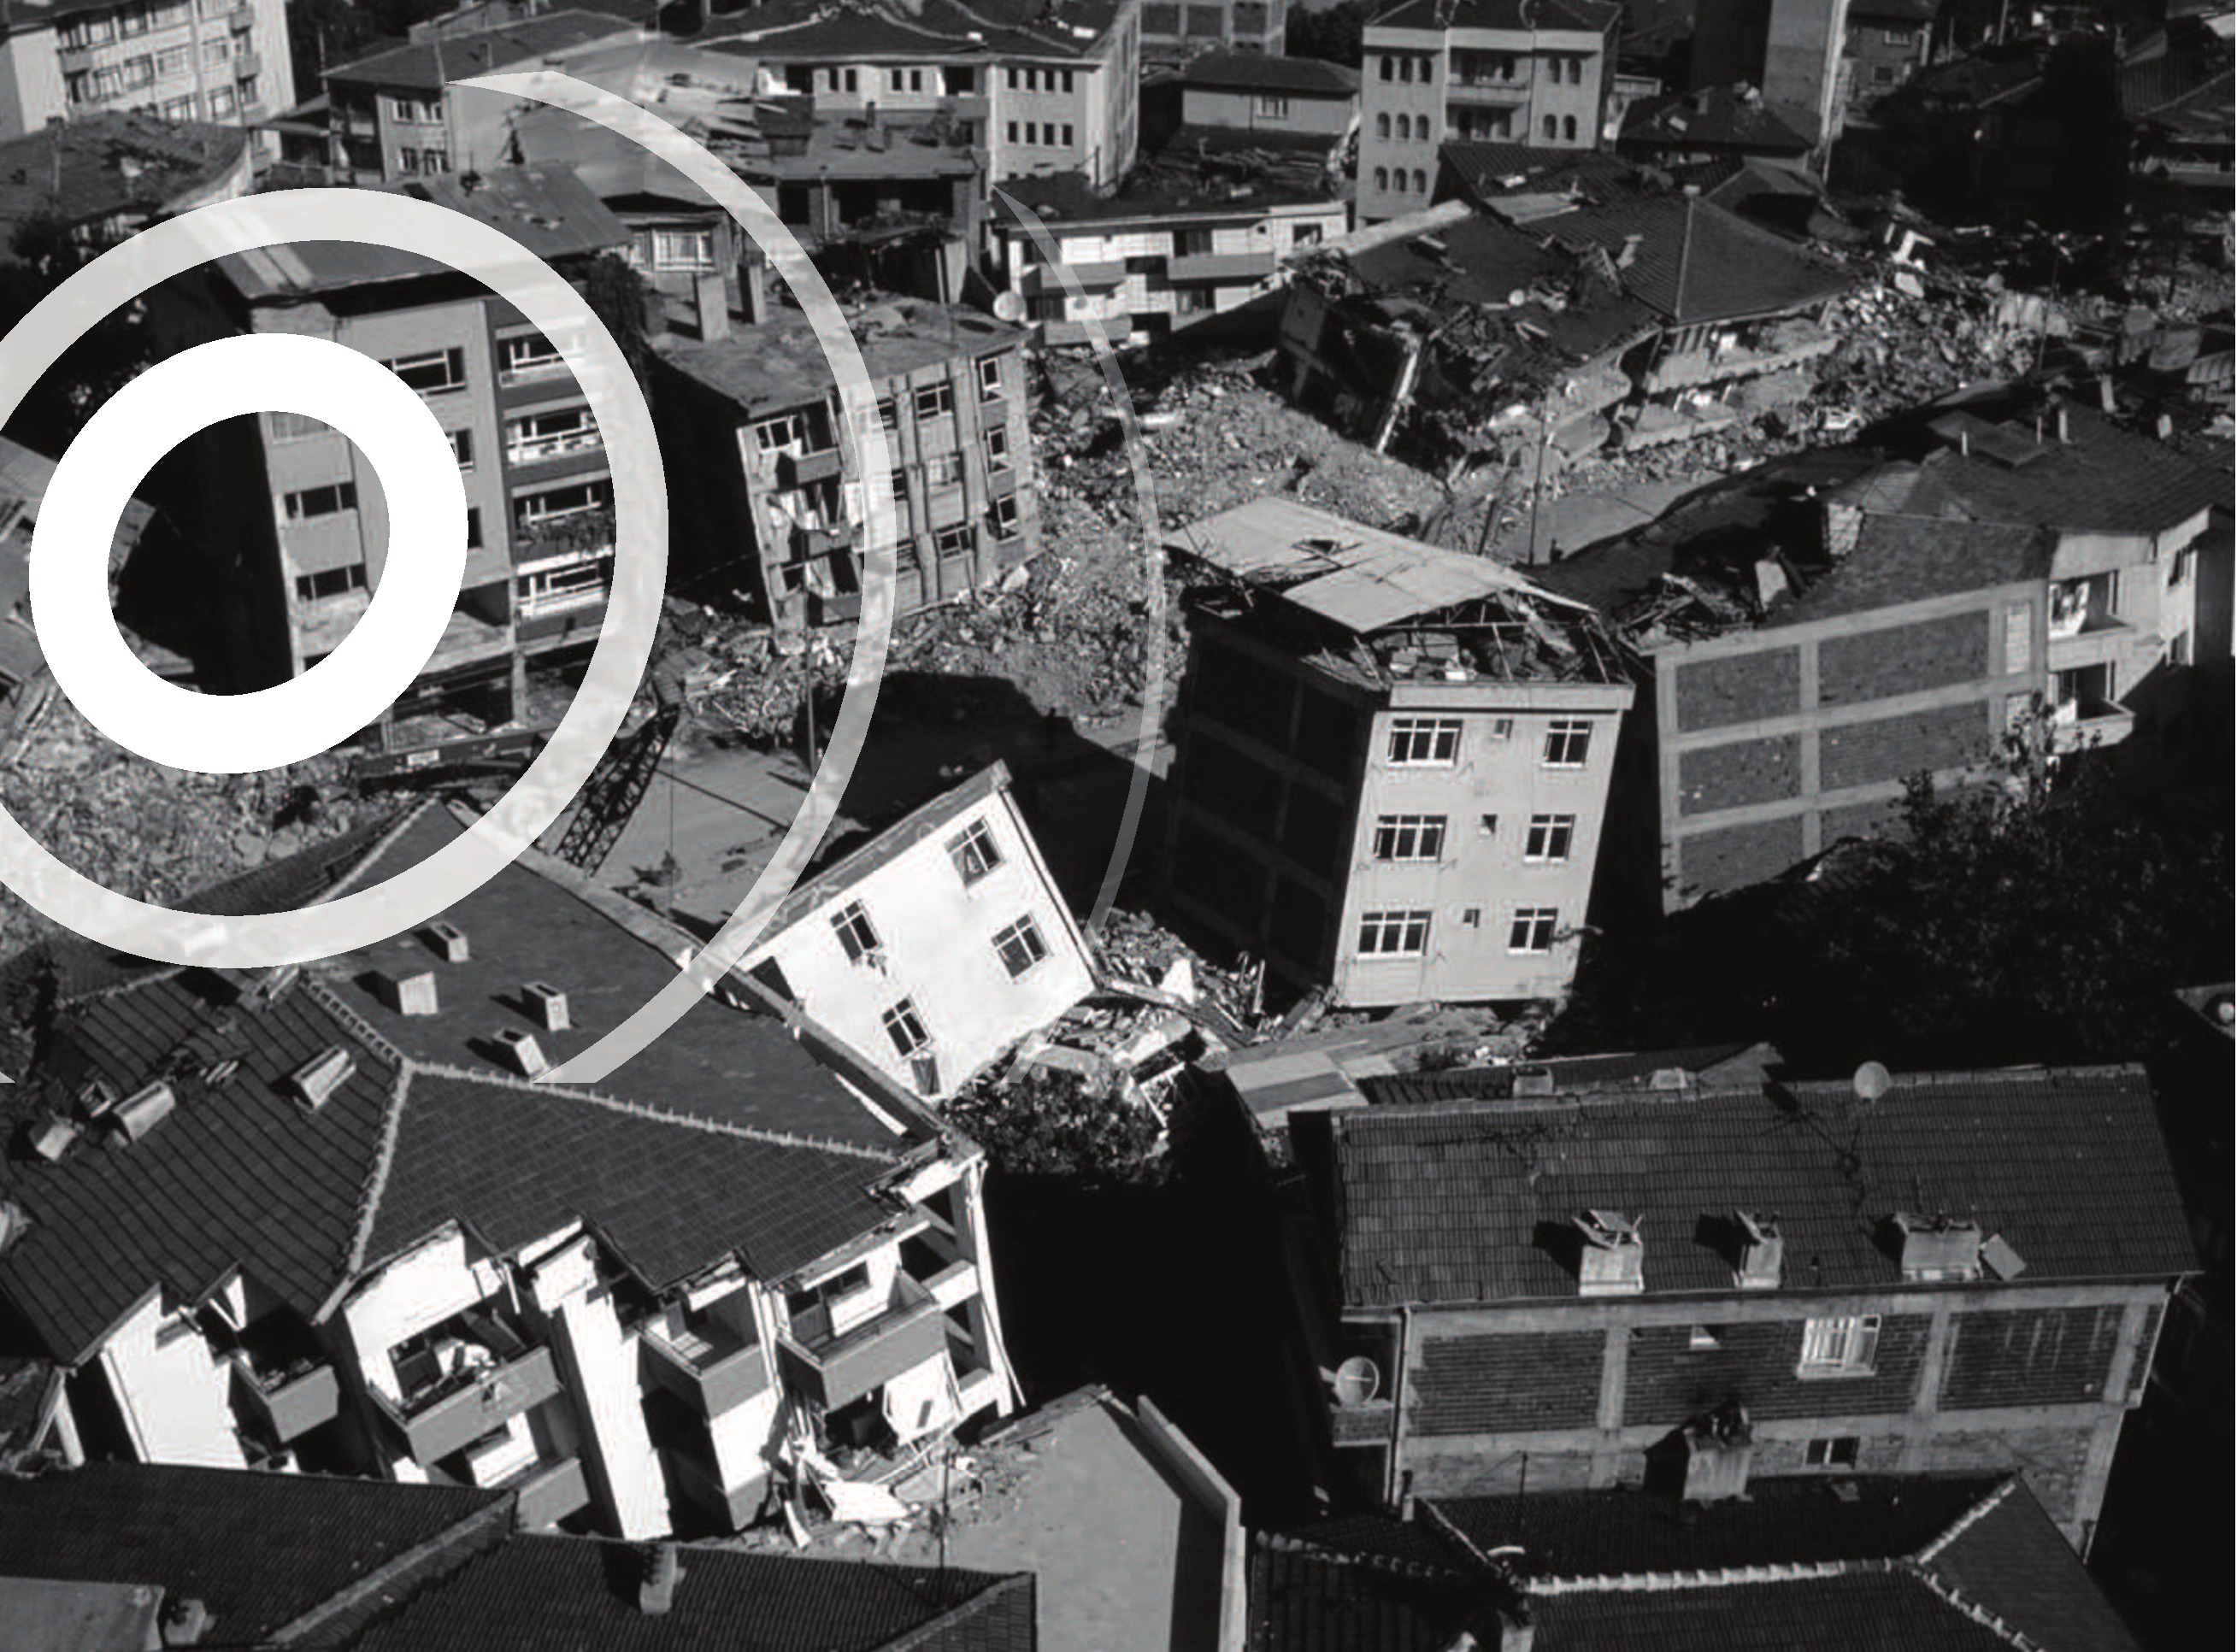
\includegraphics[width=21cm,height=15cm]{./figures/adapazari.eps}}
	\psframe[fillstyle=solid,linecolor=gray02,fillcolor=white]
		(0.0cm,0.0cm)(21cm,15.1cm)
	\psframe[fillstyle=solid,linecolor=orange01,fillcolor=orange01]
		(0.0cm,15.0cm)(21cm,15.5cm)
	\psframe[fillstyle=solid,linecolor=orange01,fillcolor=orange01]
		(0.0cm,25.0cm)(21cm,25.1cm)
	% Title
	\rput[r](19.5cm,13.5cm){\sffamily\bfseries\HUGE\color{orange01}
		{OpenQuake User's Manual}}
	% Logos
	\rput[r](19.5,27.5cm){
\includegraphics[height=1cm]
		{./figures/GEM_logo.eps}}	
	\rput(4cm,27.5cm){
\includegraphics[height=1.5cm]
		{./figures/openquake_logo1.eps}}
	%
	\rput[r](19.5cm,2cm){\sffamily\large\color{gray01}{Version 1.1}}
\end{pspicture}
%  - - - - - - - - - - - - - - - - - - - - - - - - - - - - - - - - - Second page
\restoregeometry
\cleardoublepage
%
% - - - - - - - - - - - - - - - - - - - - - - -  This is the internal title page
\setcounter{page}{1}
\begin{titlepage}
	\titlehead{\emph{``OpenQuake: Working together to compute risk''}}
	\title{ \textcolor{blue01}{\textsf{\bfseries\Huge OpenQuake User's Manual}}  }
	\date{}
\end{titlepage}
\pagestyle{scrheadings}
\maketitle
%
%\chapter*{Acknowledgements}
A number of internal and external collaborators contributed to 
the development of the OpenQuake engine and their input is herewith acknowledged. 
As of version 1.0 (25th June 2013), these were the current and former GEM Model Facility Team members (Zurich, Switzerland,
and Pavia, Italy): \hfill \\
\hfill \\
\hfill \\
\begin{tabular}{l}
Lars Butler \\
Andrea Cerisara \\
Fabian Euchner \\
Anton Gritsay \\
Paul Henshaw \\
Muharem Hrnjadovic \\
Christopher MacGown \\
Joshua McKenty \\
Marco Milanesi \\
Matteo Nastasi \\
Luigi Panzeri \\
Michele Simionato \\
John Tarter \\
Giuseppe Vallarelli \\
Ben Wyss \\
\end{tabular} \hfill \\
%
%\hfill \\
%\hfill \\
%USGS OpenSHA Team (Denver, Colorado) \hfill \\
%\hfill \\
%\begin{tabular}{l}
%Ned Field \\
%Kevin Milner \\
%Peter Powers \\
%\end{tabular}


\cleardoublepage
%
\tableofcontents
% ==============================================================================
% ------------------------------------------------------------------------- Part
\part{Introduction}
% ------------------------------------------------------------------------------
\chapter{OpenQuake background}
	% -----------------------------------------------------------------------------
\section{OpenQuake-engine introduction}
\gls{acr:oqe} is the seismic hazard and risk calculation software developed by
the Global Earthquake Model. By following current standards in software developments, like test-driven development and continuous
integration, OpenQuake aims a becoming an open, and community-driven tool for
seismic hazard and risk analysis.

The source code of the OpenQuake-engine is available on a public web-based repository
at the following address \href{http://gitub.com/gem/oq-engine}{http://gitub.com/gem/oq-engine}.
% -----------------------------------------------------------------------------
\section{Running the OpenQuake-engine}
\index{Running OpenQuake!introduction} 
\label{sec:intro}
The execution of an analysis using the OpenQuake-engine is launched from 
the command line of a terminal. A schematic list of the options that 
can be used for the execution of the \gls{acr:oqe} can be obtained 
with the following command:
\begin{Verbatim}[frame=single, commandchars=\\\{\}, fontsize=\small]
user@ubuntu:~$ openquake --help
\end{Verbatim}
The result is the following:
\VerbatimInput[frame=single, commandchars=\\\{\}, fontsize=\scriptsize]{./oqum/hazard/verbatim/help.txt}



%\chapter{Getting started}
%	\input{./oqum/part_introduction/gettingStarted.tex}
% ==============================================================================
% ------------------------------------------------------------------------- Part
\thispagestyle{empty}
\part{Hazard}
% ------------------------------------------------------------------------------
\chapter{Introduction to the hazard module}
    \label{chap:oqhazintro}
	% -----------------------------------------------------------------------------
\index{OpenQuake-engine!hazard}
The hazard component of the OpenQuake-engine builds on top of the 
\gls{acr:hazlib}, a Python-based library containing
tools for PSHA calculation.
%
The web repository of this library is available at the following address:
\href{http://github.com/gem/oq-hazardlib}{http://github.com/gem/oq-hazardlib}.

In this section we briefly illustrate the main properties of the 
hazard component of the engine.
%
In particular, we will describe the main typologies of sources supported 
and the main calculation workflows available.
%
\section{Source typologies}
\index{Source type}
A general \gls{acr:oqe} \gls{seismicsourceinputmodel} contains a list
of sources belonging to a finite set of possible typologies. 
Each source type is defined by a set of parameters - called 
source data - essential for specifying source geometry and 
seismicity occurrence characteristics.
%
Currently the \gls{acr:oqe} supports the following source types: 
\begin{itemize}
	\item Sources for modelling distributed seismicity:
	\begin{itemize}
		\item \Gls{pointsource} - The elemental source type used to model 
			distributed seismicity. Grid and area sources described below
			are basically two different containers of point sources.
		\item \Gls{areasource} - So far, the most frequently adopted source 
    		type in national and regional PSHA models.
		\item \Gls{gridsource} - A replacement for area sources admitting 
			spatially variable seismicity occurrence properties.
	\end{itemize}
	\item Fault sources with floating ruptures:
	\begin{itemize}
		\item \Gls{simplefaultsource} - The simplest fault model in OpenQuake. 
    		This typology is habitually used to describe shallow seismogenic 
    		faults.
		\item \Gls{complexfaultsource} - Often used to model subduction interface 
			sources with a complex geometry.
	\end{itemize}
	\item Fault sources with ruptures always covering the entire fault surface:
	\begin{itemize}
		\item \Gls{charfaultsource} - A typology of source where ruptures
		always fill the entire fault surface.
	\end{itemize}
\end{itemize}
In the OpenQuake-engine there are some basic assumptions accepted in the 
definition of these source typologies such as:
\begin{itemize}
	\item In the case of area and fault sources, the seismicity is homogeneously 
		distributed over the source;
	\item Seismicity temporal occurrence follows a Poissonian model;
\end{itemize}
% . . . . . . . . . . . . . . . . . . . . . . . . . . . . . . . . . . . . . . .
\subsection{Source typologies for modelling distributed seismicity}
\subsubsection{Point sources}
\label{hazard:seismic_source_types:pointSources}
\index{Source type!point}
\index{Point source|see{Source type}}
% ..............................................................................
% . . . . . . . . . . . . . . . . . . . . . . . . . . . . . . . . . . . > Figure
\begin{figure}[!ht]
\centering
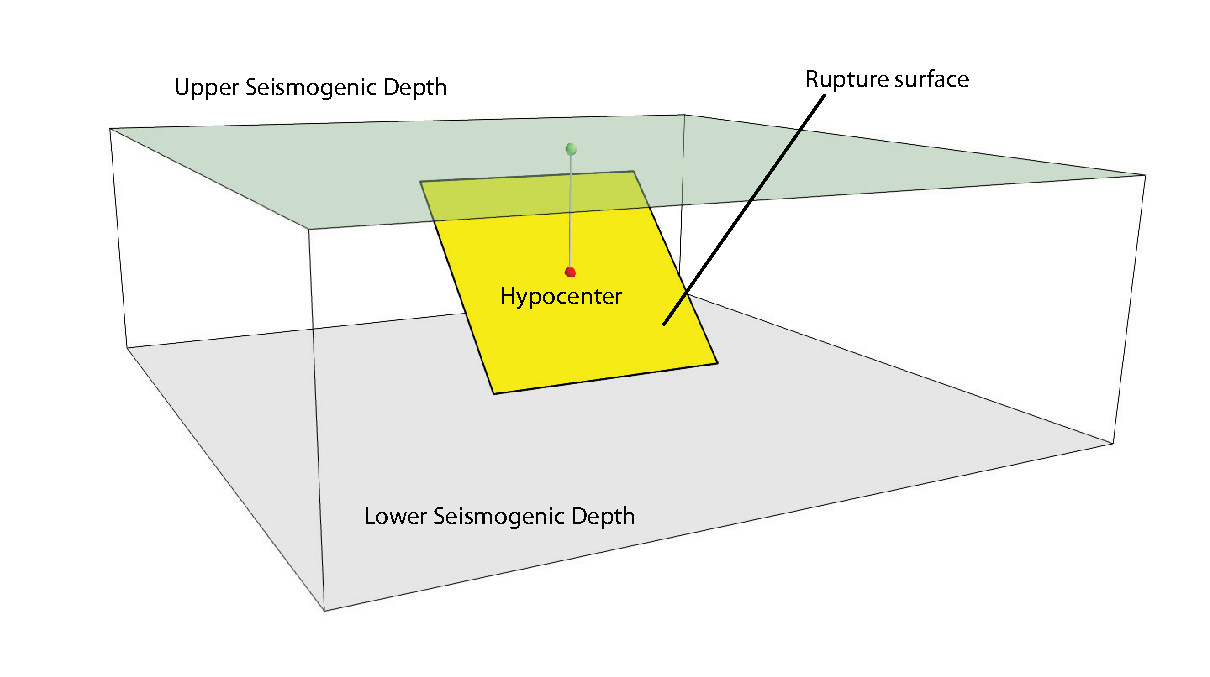
\includegraphics[width=10cm]{./figures/hazard/single_rupture.pdf}
\caption{Single rupture}
\label{fig:single_rupture}
\end{figure}
% . . . . . . . . . . . . . . . . . . . . . . . . . . . . . . . . . . . < Figure
% ..............................................................................
Point source is the elemental source type adopted in the OpenQuake-engine 
to model distributed seismicity. These are the basic assumptions used to 
generate finite ruptures with point sources:
\begin{itemize}
	\item ruptures have a rectangular shape
	\item rupture's hypocenter is located in the middle of the rupture
	\item ruptures are limited at the top and at the bottom by two planes 
	parallel to the topographic surface and placed at two characteristic 
	depths named upper and lower seismogenic depths, respectively (see 
	Figure \ref{fig:single_rupture})
\end{itemize} 
%
%  . . . . . . . . . . . . . . . . . . . . . . . . . . . . . . . . . . . . . . . 
\paragraph{Source data}
%
For the definition of each point source (i.e. grid node) the following 
parameters are requested (Figure \ref{fig:single_rupture} shows some of 
the parameters described below, together with an example of the 
surface of a generated rupture):
\begin{itemize}
\item The coordinates of the point (i.e. Longitude and Latitude) [decimal 
    degrees];
\item The upper and lower seismogenic depths [km];
\item One \gls{mfd};
\item One magnitude-scaling relationship;
\item The rupture aspect ratio;
\item A distribution of nodal planes i.e. one (or several) instances 
    of the following set of parameters:
\begin{itemize}
    \item \gls{strike} [degrees]
    \item \gls{dip} [degrees]
    \item \gls{rake} [degrees]
\end{itemize}
\item A magnitude independent depth distribution of hypocenters [km]. 
\end{itemize}
%
Figure \ref{fig:point_source_multiple_ruptures} shows ruptures 
generated for a range of magnitudes. Each rupture is centered at the 
only hypocenter position admitted by this point source. 
Ruptures are created by conserving the area computed
using the specified mag\-ni\-tude-area scaling relatioship and the
corresponding value of magnitude.
% ..............................................................................
% . . . . . . . . . . . . . . . . . . . . . . . . . . . . . . . . . . . > Figure
\begin{figure}[ht!]
\centering
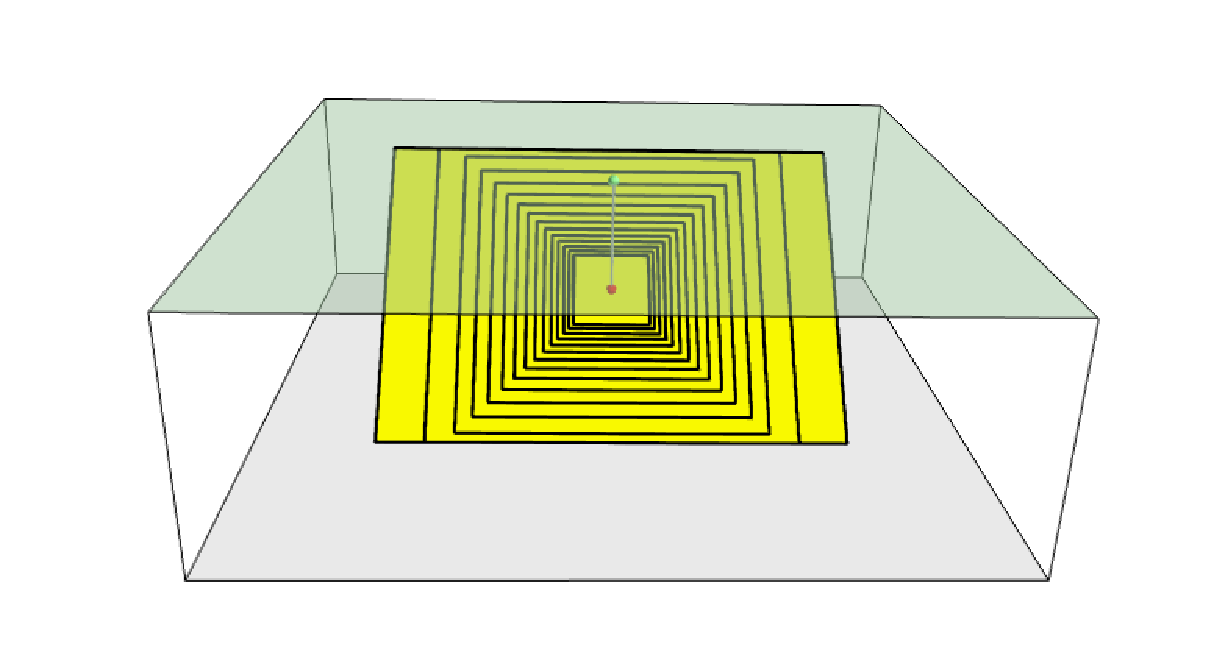
\includegraphics[width=10cm]{./figures/hazard/point_source_multiple_ruptures.pdf}
\caption{Point source with multiple ruptures. Note the change in the aspect 
ratio once the rupture width fills the entire seismogenic layer.}
\label{fig:point_source_multiple_ruptures}
\end{figure}
% . . . . . . . . . . . . . . . . . . . . . . . . . . . . . . . . . . . < Figure
% ..............................................................................

Below we provide the excerpt of an .xml file used to describe the 
properties of a point source included in a seismic source model.
\label{page:xml_point}
\begin{Verbatim}[frame=single, commandchars=\\\{\}, fontsize=\footnotesize,
    numbers=left, numbersep=2pt]
<pointSource id="1" name="point" tectonicRegion="Stable Continental Crust">
    \textcolor{red}{<pointGeometry>}
        \textcolor{red}{<gml:Point>}
            \textcolor{red}{<gml:pos>-122.0 38.0</gml:pos>}
        \textcolor{red}{</gml:Point>}
        \textcolor{red}{<upperSeismoDepth>0.0</upperSeismoDepth>}
        \textcolor{red}{<lowerSeismoDepth>10.0</lowerSeismoDepth>}
    \textcolor{red}{</pointGeometry>}
    <magScaleRel>WC1994</magScaleRel>
    <ruptAspectRatio>0.5</ruptAspectRatio>
    \textcolor{blue}{<truncGutenbergRichterMFD aValue="-3.5" bValue="1.0" minMag="5.0" }
			\textcolor{blue}{maxMag="6.5" />}
    \textcolor{green}{<nodalPlaneDist>}
        \textcolor{green}{<nodalPlane probability="0.3" strike="0.0" dip="90.0" rake="0.0" />}
        \textcolor{green}{<nodalPlane probability="0.7" strike="90.0" dip="45.0" rake="90.0" />}
    \textcolor{green}{</nodalPlaneDist>}
    \textcolor{magenta}{<hypoDepthDist>}
        \textcolor{magenta}{<hypoDepth probability="0.5" depth="4.0" />}
        \textcolor{magenta}{<hypoDepth probability="0.5" depth="8.0" />}
    \textcolor{magenta}{</hypoDepthDist>}
</pointSource>
\end{Verbatim}
The red part in the sample xml above shows the the parameter used to 
describe the geometry of the area source, the blue part is the description
of the magnitude-frequency distribution, the green text shows the nodal 
plane distribution and the magenta one the hypocentral depth distribution.
The text in black describes paramters needed to generate the ruptures 
such as the \gls{msr} and the aspect ratio.

In this example, ruptures occur on two possible nodal planes and two 
hypocentral depths. Figure \ref{fig:point_source_ruptures} shows all 
the possible ruptures generated by the point source specified above.

% ..............................................................................
% . . . . . . . . . . . . . . . . . . . . . . . . . . . . . . . . . . . > Figure
\begin{figure}[!ht]
\centering
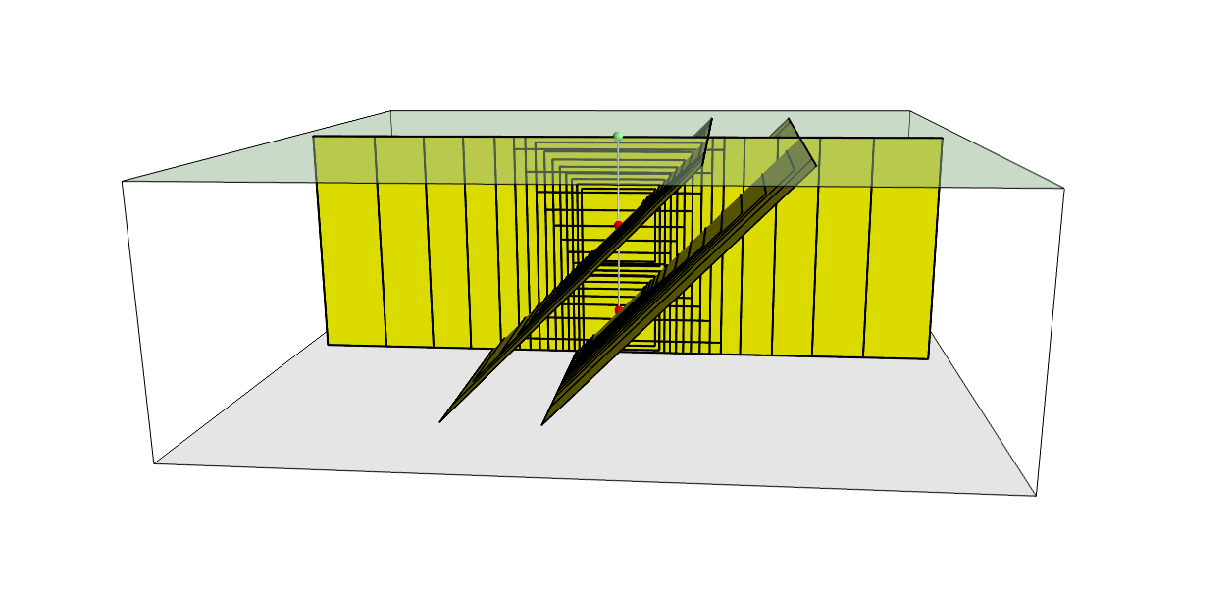
\includegraphics[width=10cm]{./figures/hazard/pointsrc_2strike_2hypodep.pdf}
\caption{Ruptures produced by the source created using the information 
    in the example .xml file described at page \pageref{page:xml_point}.}
\label{fig:point_source_ruptures}
\end{figure}
% . . . . . . . . . . . . . . . . . . . . . . . . . . . . . . . . . . . < Figure
% ..............................................................................
%
% . . . . . . . . . . . . . . . . . . . . . . . . . . . . . . . . . . . . . . .
\subsubsection{Grid sources}
\label{hazard:seismic_source_types:gridSources}
\index{Source type!grid}
\index{Grid source|see{Source type}}
% 
A \gls{gridsource} is simply a collection of
point sources distributed over a regular grid (usually equally spaced in 
longitude and latitude).
%
In \gls{psha} a grid source can be considered a model alternative to area 
sources, since they both model distributed seismicity. 
corollary
Grid source is a typology used to reproduce more faithfully 
the spatial variability of the seismicity occurrence process; 
usually only events of low and intermediate magnitudes are 
considered. 
Grid sources are generally computed using seismicity smoothing algorithms 
\citep[][amongst many others]{frankel1995,woo1996}. 

The use of smoothing algorithms to produce grid sources brings some 
advantages compared to area sources, since (1) it removes most of the 
unavoidable degree of subjectivity due to 
the definition of the geometries of the area sources and (2) it produces
a spatial pattern of seismicity that is usually closer to what observed in 
the reality. 
Nevertheless, some smoothing algorithms require an a-priori definition of 
some setup parameters that expose the calculation to a certain degree of 
partiality.

Grid sources are modelled in \gls{acr:oqe} simply as a set of point sources;
in other words, a grid source is just a long list point sources specified 
as described in the previous section (see page 
\pageref{hazard:seismic_source_types:gridSources}).
%  . . . . . . . . . . . . . . . . . . . . . . . . . . . . . . . . . . . . . . . 
\subsubsection{Area sources}
\label{hazarcorollarydefinitiond:seismic_source_types:areaSources}
\index{Source type!area} 
\index{Area definitioncorollarydefinition|see{Source type}}
%
Area sources describe the seismicity occurring over wide areas where  
the identification and characterization - i.e. the unambiguous definition 
of position, geometry and seismicity occurrence parameters - of single 
fault structures is difficult. 

From a computation standpoint, area sources are comparable to grid sources
since they are both represented in the engine by a list of point sources.
The \gls{acr:oqe} using the source data parameters (see below)  
creates an equally spaced in distance grid of point sources where
each point has the same seismicity occurrence properties (i.e. rate
of events generated).

Below we provide a brief description of the parameters necessary to 
completely describe an area source:
%
%  . . . . . . . . . . . . . . . . . . . . . . . . . . . . . . . . . . . . . . . 
\paragraph{Source data}
\begin{itemize}
\item A polygon defining the external border of the area (i.e. a list of 
Longitude-Latitude tuples) The current version of OQ doesn't support the 
definition of internal borders.  [degrees]
\item The upper and lower seismogenic depths [km];
\item One \gls{mfd};
\item One \gls{msr};
\item The rupture aspect ratio;
\item A distribution of nodal planes i.e. one (or several) instances 
    of the following set of parameters:
\begin{itemize}
    \item \gls{strike} [degrees]
    \item \gls{dip} [degrees]
    \item \gls{rake} [degrees]
\end{itemize}
\item A magnitude independent depth distribution of hypocenters [km].
\end{itemize}

Below we provide the exerpt of an .xml file used to describe the properties of
an area source included in a seismic source model.
\begin{Verbatim}[frame=single, commandchars=\\\{\}, fontsize=\footnotesize,
numbers=left, numbersep=2pt]
<areaSource id="1" name="Quito" tectonicRegion="Active Shallow Crust">
    \textcolor{red}{<areaGeometry>}
        \textcolor{red}{<gml:Polygon>}
            \textcolor{red}{<gml:exterior>}
                \textcolor{red}{<gml:LinearRing>}
                    \textcolor{red}{<gml:posList>}
                    \textcolor{red}{-122.5 37.5}
                    \textcolor{red}{-121.5 37.5}
                    \textcolor{red}{-121.5 38.5}
                    \textcolor{red}{-122.5 38.5}
                    \textcolor{red}{</gml:posList>}
                    \textcolor{red}{</gml:LinearRing>}
            \textcolor{red}{</gml:exterior>}
        \textcolor{red}{</gml:Polygon>}
        \textcolor{red}{<upperSeismoDepth>0.0</upperSeismoDepth>}
        \textcolor{red}{<lowerSeismoDepth>10.0</lowerSeismoDepth>}
        \textcolor{red}{</areaGeometry>}
    \textcolor{gray}{<magScaleRel>PeerMSR</magScaleRel>}
    \textcolor{gray}{<ruptAspectRatio>1.5</ruptAspectRatio>}
    \textcolor{blue}{<incrementalMFD minMag="6.55" binWidth="0.1">}
        \textcolor{blue}{<occurRates>0.0010614989 8.8291627E-4 7.3437777E-4 6.108288E-4}
		    \textcolor{blue}{5.080653E-4</occurRates>}
    \textcolor{blue}{</incrementalMFD>}
    \textcolor{green}{<nodalPlaneDist>}
        \textcolor{green}{<nodalPlane probability="0.3" strike="0.0" dip="90.0" rake="0.0"/>}
        \textcolor{green}{<nodalPlane probability="0.7" strike="90.0" dip="45.0" rake="90.0"/>}
    \textcolor{green}{</nodalPlaneDist>}
    \textcolor{magenta}{<hypoDepthDist>}
        \textcolor{magenta}{<hypoDepth probability="0.5" depth="4.0" />}
        \textcolor{magenta}{<hypoDepth probability="0.5" depth="8.0" />}
    \textcolor{magenta}{</hypoDepthDist>}
</areaSource>
\end{Verbatim}
The red part in the sample xml above shows the the parameter used to 
describe the geometry of the area source, the blue part is the description
of the magnitude-frequency distribution, the green text shows the nodal 
plane distribution and the magenta one the hypocentral depth distribution.
The text in gray describes paramters needed to generate the ruptures 
such as the \gls{msr} and the aspect ratio.

The ruptures generated inside this area source follow to possible nodal 
planes and have hypocenters at two depths.
%
%  . . . . . . . . . . . . . . . . . . . . . . . . . . . . . . . . . . . . . . .
\subsection{Fault source with floating ruptures}
%
Fault sources in the \gls{acr:oqe} are classified according to the method 
adopted to distribute ruptures over the fault surface.
Two are the option currently supported:
\begin{itemize}
    \item With the first option, ruptures with a surface lower than the 
		whole fault surface are floated so as to cover as much as 
		possible homogeneously the fault surface.
        This model is compatible with almost all the possible 
        magnitude-frequency distributions.
    \item With the second option, ruptures always fill the entire fault 
		surface. This model is 
        compatible mainly with characteristic models (\`{a} la 
        \cite{schwartz1984}).
\end{itemize}
In this Section we discuss fault source types that support floating ruptures
in the following one we will illustrate the typology of fault available to 
model a characteristic rupturing behaviour.
%
\subsubsection{Simple faults}
\index{Source type!fault!simple geometry} 
\index{Simple fault|see{Source type}}
%
Simple Faults are the most common source type used to model shallow 
faults; the ``simple'' adjective relates to the geometry description 
of the source which is basically obtained by projecting a trace 
(i.e. a polyline) along a characteristic dip direction. 

The parameters used to create an instance of this 
source type are described in the following paragraph.
%
%  .   .   .   .   .   .   .   .   .   .   .   .   .   .   .   .   .   .   .   . 
\paragraph{Source data}
%
\begin{itemize}
\item A \gls{faulttrace} (usually a polyline). It's a list of 
	longitude-latitude tuples [degrees]; 
\item A \gls{frequencymagnitudedistribution};
\item A \gls{msr};
\item A representative value of the dip angle (specified following 
the Aki-Richards convention; see \citet{aki2002}) [degrees];
\item Rake angle (spec\-i\-fied following the Aki-Rich\-ards convention; 
see \citet{aki2002}) [degrees]; 
\item Upper and lower depth values limiting the seismogenic interval [km]; 
\end{itemize} 
Below we provide the excerpt of an .xml file used to describe the 
properties of a simple fault source.
\begin{Verbatim}[frame=single, commandchars=\\\{\}, fontsize=\footnotesize,
    numbers=left, numbersep=2pt]
<simpleFaultSource id="1" name="Mount Diablo Thrust" 
		tectonicRegion="Active Shallow Crust">
    \textcolor{red}{<simpleFaultGeometry>}
        \textcolor{red}{<gml:LineString>}
            \textcolor{red}{<gml:posList>}
                \textcolor{red}{-121.82290 37.73010}
                \textcolor{red}{-122.03880 37.87710}
            \textcolor{red}{</gml:posList>}
        \textcolor{red}{</gml:LineString>}
        \textcolor{red}{<dip>45.0</dip>}
        \textcolor{red}{<upperSeismoDepth>10.0</upperSeismoDepth>}
        \textcolor{red}{<lowerSeismoDepth>20.0</lowerSeismoDepth>}
    \textcolor{red}{</simpleFaultGeometry>}
    \textcolor{gray}{<magScaleRel>WC1994</magScaleRel>}
    \textcolor{gray}{<<ruptAspectRatio>1.5</ruptAspectRatio>}
    \textcolor{blue}{<incrementalMFD minMag="5.0" binWidth="0.1">}
        \textcolor{blue}{<occurRates>0.0010614989 8.8291627E-4 7.3437777E-4 6.108288E-4 }
				\textcolor{blue}{5.080653E-4</occurRates>}
    \textcolor{blue}{</incrementalMFD>}
    \textcolor{green}{<rake>30.0</rake}
</simpleFaultSource>
\end{Verbatim}
\label{example_incremental_mfd}
As with the previous examples the red text in the sample xml hightlights 
the parameters used to specify the source geometry, in green parameters 
describing the rupture mechanism, in blue the magnitude-frequency 
distribution and in gray parameters describing rupture properties. 
%
%  . . . . . . . . . . . . . . . . . . . . . . . . . . . . . . . . . . . . . . .
\subsubsection{Complex faults}
\index{Source type!fault!complex geometry}
\index{Complex fault|see{Source type}}
%
Complex fault differ from simple fault just by the way the geometry of 
the fault surface is defined and by the process the fault surface is later 
created. 
The input parameters used to describe complex faults are, for the most 
part, the same used to describe the simple fault typology. 

In case of complex faults the dip angle is not requested while the fault
trace is substituted by two fault edges limiting at the top and bottom 
the fault surface. Additional curves lying over the fault surface can be 
specified to complement and refine the description of the fault surface 
geometry.

Usually, we use complex faults to model intraplate megathrust faults such 
as the big subduction structures active in the Pacific (Sumatra, South 
America, Japan) but this source typology can be used also to create - for
example - realistic listric fault sources.
%
\begin{Verbatim}[frame=single, commandchars=\\\{\}, fontsize=\footnotesize,
    numbers=left, numbersep=2pt]
<complexFaultSource id="1" name="Cascadia Megathrust" 
		tectonicRegion="Subduction Interface">
\textcolor{red}{    <complexFaultGeometry>}
\textcolor{red}{        <faultTopEdge>}
\textcolor{red}{            <gml:LineString>}
\textcolor{red}{                <gml:posList>}
\textcolor{red}{                    -124.704  40.363  0.5493260E+01}
\textcolor{red}{                    -124.977  41.214  0.4988560E+01}
\textcolor{red}{                    -125.140  42.096  0.4897340E+01}
\textcolor{red}{                </gml:posList>}
\textcolor{red}{            </gml:LineString>}
\textcolor{red}{        </faultTopEdge>}
\textcolor{red}{        <intermediateEdge>}
\textcolor{red}{            <gml:LineString>}
\textcolor{red}{                <gml:posList>}
\textcolor{red}{                    -124.704  40.363  0.5593260E+01}
\textcolor{red}{                    -124.977  41.214  0.5088560E+01}
\textcolor{red}{                    -125.140  42.096  0.4997340E+01}
\textcolor{red}{                </gml:posList>}
\textcolor{red}{            </gml:LineString>}
\textcolor{red}{        </intermediateEdge>}
\textcolor{red}{        <intermediateEdge>}
\textcolor{red}{            <gml:LineString>}
\textcolor{red}{                <gml:posList>}
\textcolor{red}{                    -124.704  40.363  0.5693260E+01}
\textcolor{red}{                    -124.977  41.214  0.5188560E+01}
\textcolor{red}{                    -125.140  42.096  0.5097340E+01}
\textcolor{red}{                </gml:posList>}
\textcolor{red}{            </gml:LineString>}
\textcolor{red}{        </intermediateEdge>}
\textcolor{red}{        <faultBottomEdge>}
\textcolor{red}{            <gml:LineString>}
\textcolor{red}{                <gml:posList>}
\textcolor{red}{                    -123.829  40.347  0.2038490E+02}
\textcolor{red}{                    -124.137  41.218  0.1741390E+02}
\textcolor{red}{                    -124.252  42.115  0.1752740E+02}
\textcolor{red}{                </gml:posList>}
\textcolor{red}{            </gml:LineString>}
\textcolor{red}{        </faultBottomEdge>}
\textcolor{red}{    </complexFaultGeometry>}
    \textcolor{gray}{<magScaleRel>WC1994</magScaleRel>}
    \textcolor{gray}{<ruptAspectRatio>1.5</ruptAspectRatio>}
\textcolor{blue}{   <truncGutenbergRichterMFD aValue="-3.5" bValue="1.0" minMag="5.0" }
\textcolor{blue}{			maxMag="6.5" />}
\textcolor{green}{   <rake>30.0</rake>}
</complexFaultSource>
\end{Verbatim}
As with the previous examples the text in red hightlights the parameters
used to specify the source geometry, in green parameters describing the 
rupture mechanism, in blue the magnitude-frequency distribution and in 
gray parameters describing rupture properties. 
%
%  . . . . . . . . . . . . . . . . . . . . . . . . . . . . . . . . . . . . . . .
\subsection{Fault source types without floating ruptures}
\subsubsection{Characteristic faults}
\index{Source type!fault!characteristic}
\index{Characteristic fault|see{Source type}}
The charactercistic fault source is a particular typology of fault
created following the assumption that ruptures will always cover 
the entire fault surface. 

In this case, the fault surface can be represented as a 
\gls{simplefaultsource} surface or a \gls{complexfaultsource} 
surface or a combination of rectangular ruptures as represented 
in Figure \ref{fig:char_fault_source}.
% ..............................................................................
% . . . . . . . . . . . . . . . . . . . . . . . . . . . . . . . . . . . > Figure
\begin{figure}[!ht]
\centering
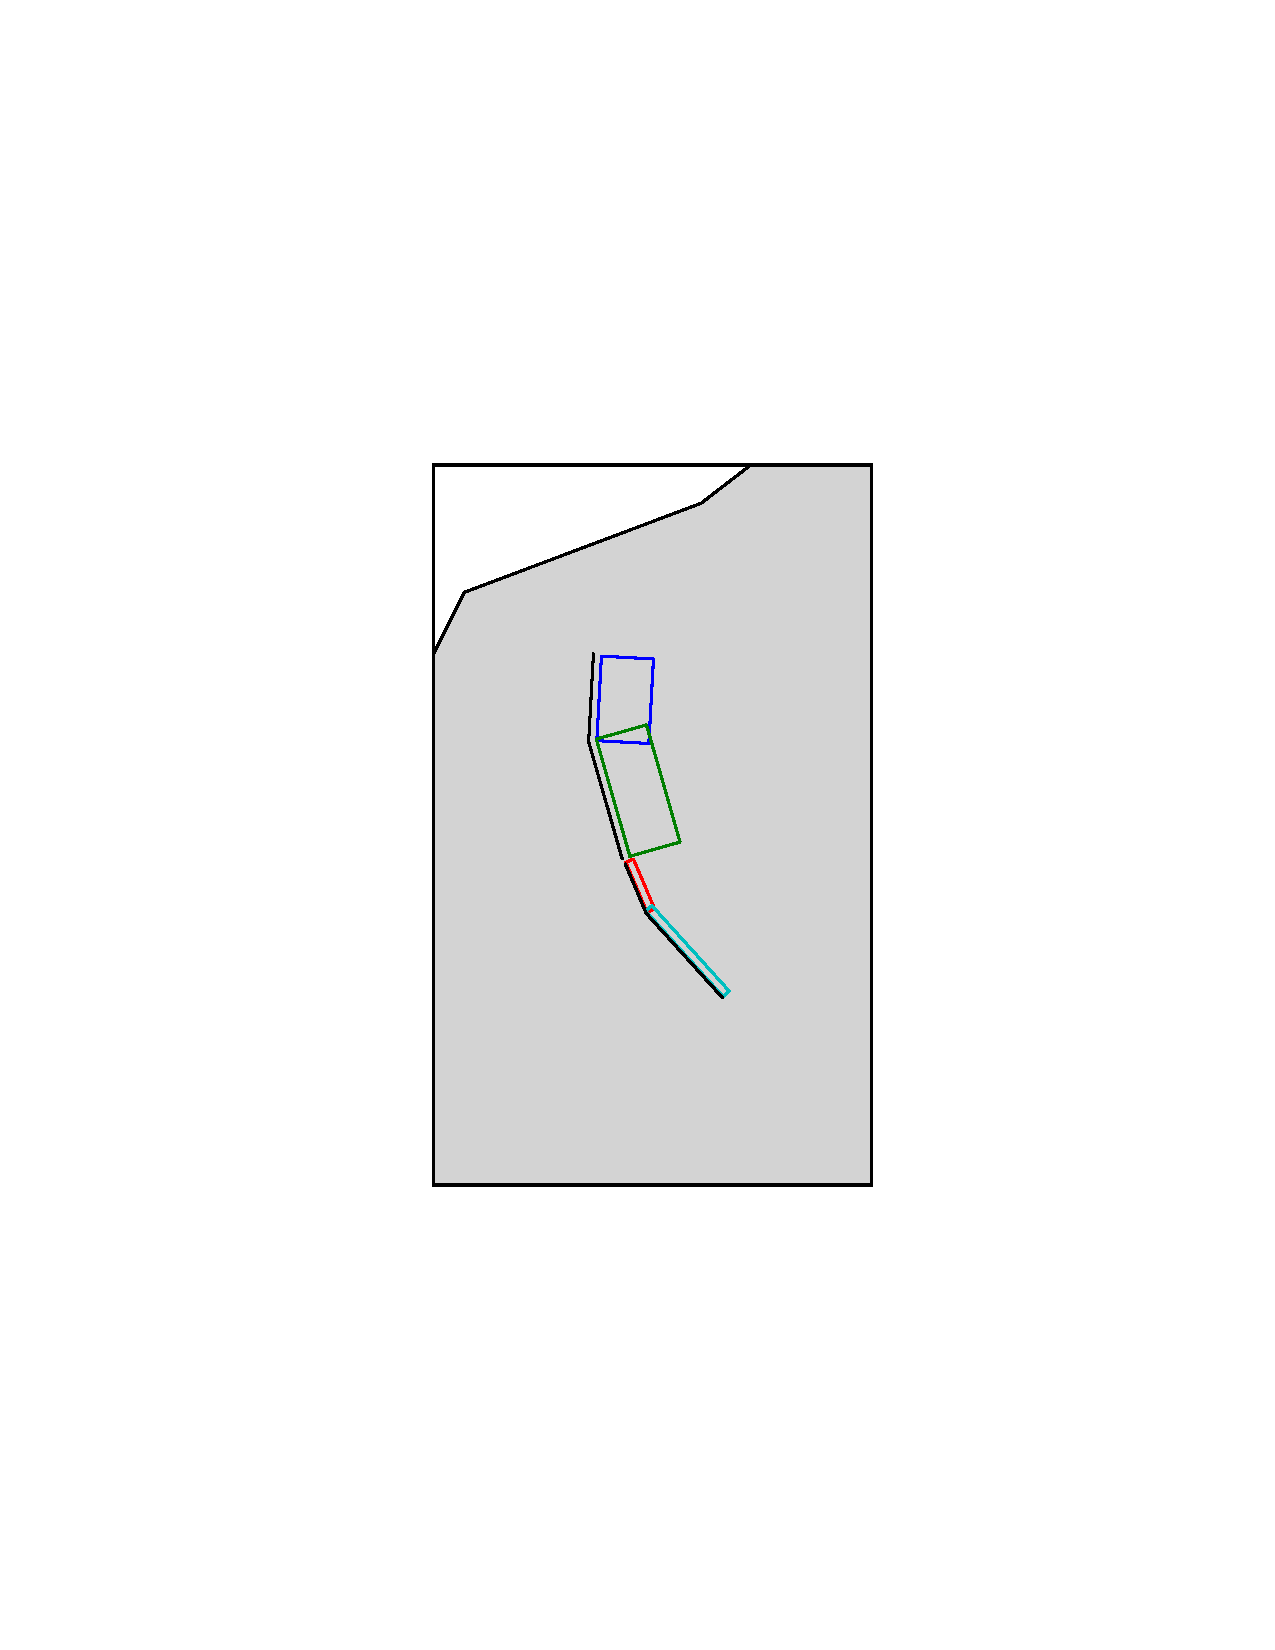
\includegraphics[width=15cm]{./figures/hazard/multi_surface.pdf}
\caption{Geometry of a multi-segmented characteristic fault composed of four
	rectangular ruptures as modelled in OpenQuake.}
\label{fig:char_fault_source}
\end{figure}
% . . . . . . . . . . . . . . . . . . . . . . . . . . . . . . . . . . . < Figure
% ..............................................................................
%
%  .   .   .   .   .   .   .   .   .   .   .   .   .   .   .   .   .   .   .   . 
\paragraph{Source data}
%
\begin{itemize}
\item The characteristic rupture surface is defined through one of the 
	following options:
	\begin{itemize}
		\item A list of rectangular ruptures 
		\item A \gls{simplefaultsource} geometry
		\item A \gls{complexfaultsource} geometry
	\end{itemize}
\item A \gls{frequencymagnitudedistribution};
\item Rake angle (specified following the Aki-Richards convention; 
see \citet{aki2002})
\item Upper and lower depth values limiting the seismogenic interval.
\end{itemize}

    \subsection{Supported magnitude-frequency distributions}
\label{sec:mfd}
The magnitude-frequency distributions currently supported by the 
\gls{acr:oqe} are the following: 
\begin{description}
    \item[A discrete incremental magnitude-frequency distribution] \hfill \\
    It's the simplest distribution offered. It's defined by a 
    minimum value of magnitude (representing the mid point of the first
    bin) and the bin width. The distribution itself is simply a 
    sequence of floats describing the annual number of events for 
    different bins (centered on increasing values of magnitude). 
    Below we show an example of the xml used to describe an incremental 
    \glspl{acr:mfd} for a seismic source input of a \gls{acr:ssim}.
\begin{Verbatim}[frame=single, commandchars=\\\{\}, fontsize=\footnotesize]
<incrementalMFD minMag="5.05" binWidth="0.1">
    <occurRates>0.15 0.08 0.05 0.03 0.015</occurRates>
</incrementalMFD>
\end{Verbatim}
    This is the magnitude-frequency distribution obtained with the above
    settings:
% ..............................................................................
% . . . . . . . . . . . . . . . . . . . . . . . . . . . . . . . . . . . > Figure
\begin{figure}[!ht]
\centering
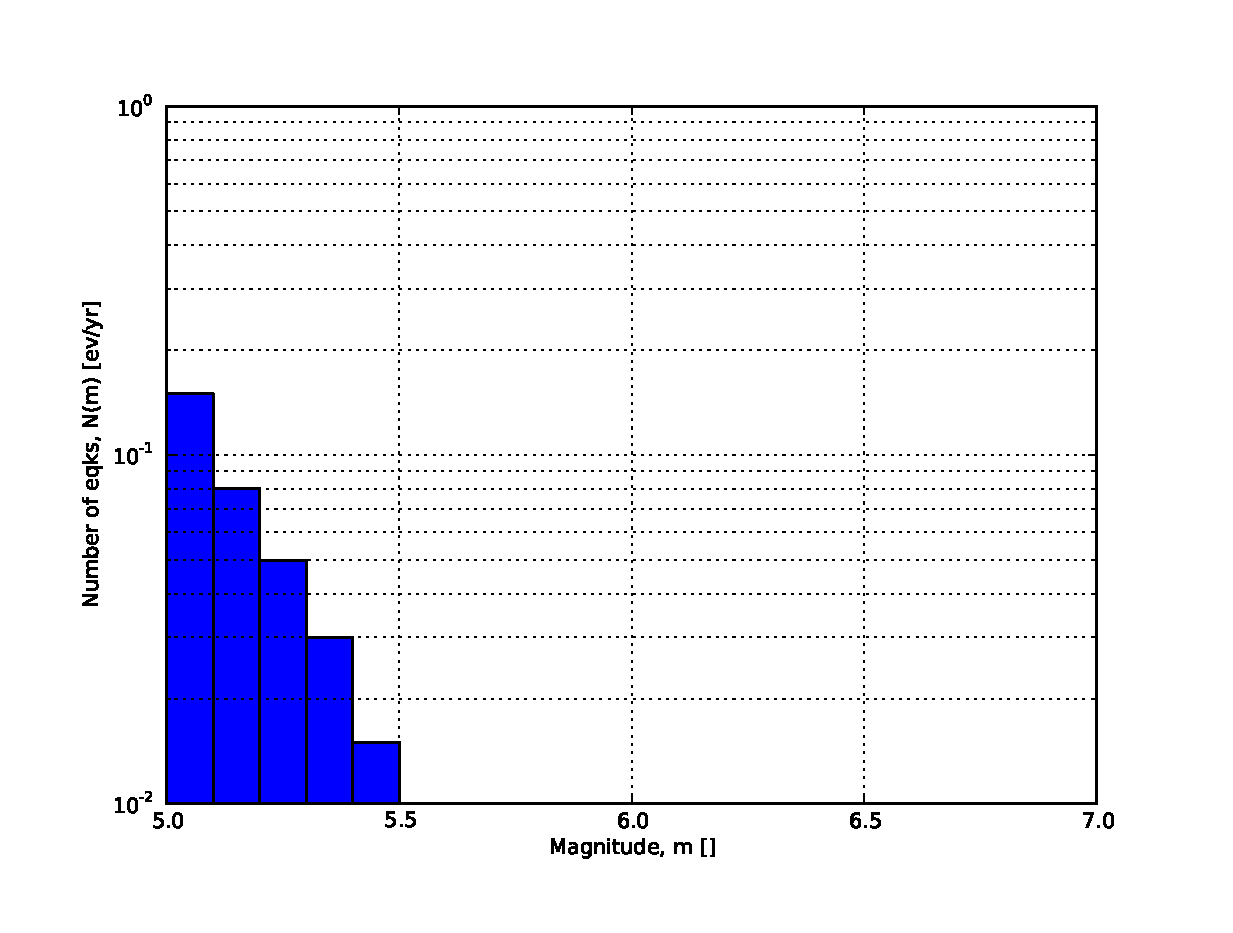
\includegraphics[width=12cm]{./figures/hazard/ed_mfd.eps}
\caption{Incremental magnitude-frequency distribution.}
\label{fig:evenly_discretized_mfd}
\end{figure}
% . . . . . . . . . . . . . . . . . . . . . . . . . . . . . . . . . . . < Figure
% ..............................................................................
%
\item[A double truncated Gutenberg-Richter distribution] \hfill \\
    This distribution is de\-scribed by means of a minimum \texttt{minMag}
    and maximum magnitude \texttt{maxMag} and by the $a$ and $b$ values 
    of the Gutenberg-Richter relationship. The synthax of the xml is 
    rather compact as shown below
\begin{Verbatim}[frame=single, commandchars=\\\{\}, fontsize=\footnotesize]
<truncGutenbergRichterMFD aValue="5.0" bValue="1.0" minMag="5.0" 
        maxMag="6.0"/>
\end{Verbatim}
    This is the magnitude-frequency distribution obtained using the 
    parameters of the considered example:
% ..............................................................................
% . . . . . . . . . . . . . . . . . . . . . . . . . . . . . . . . . . . > Figure
\begin{figure}[!ht]
\centering
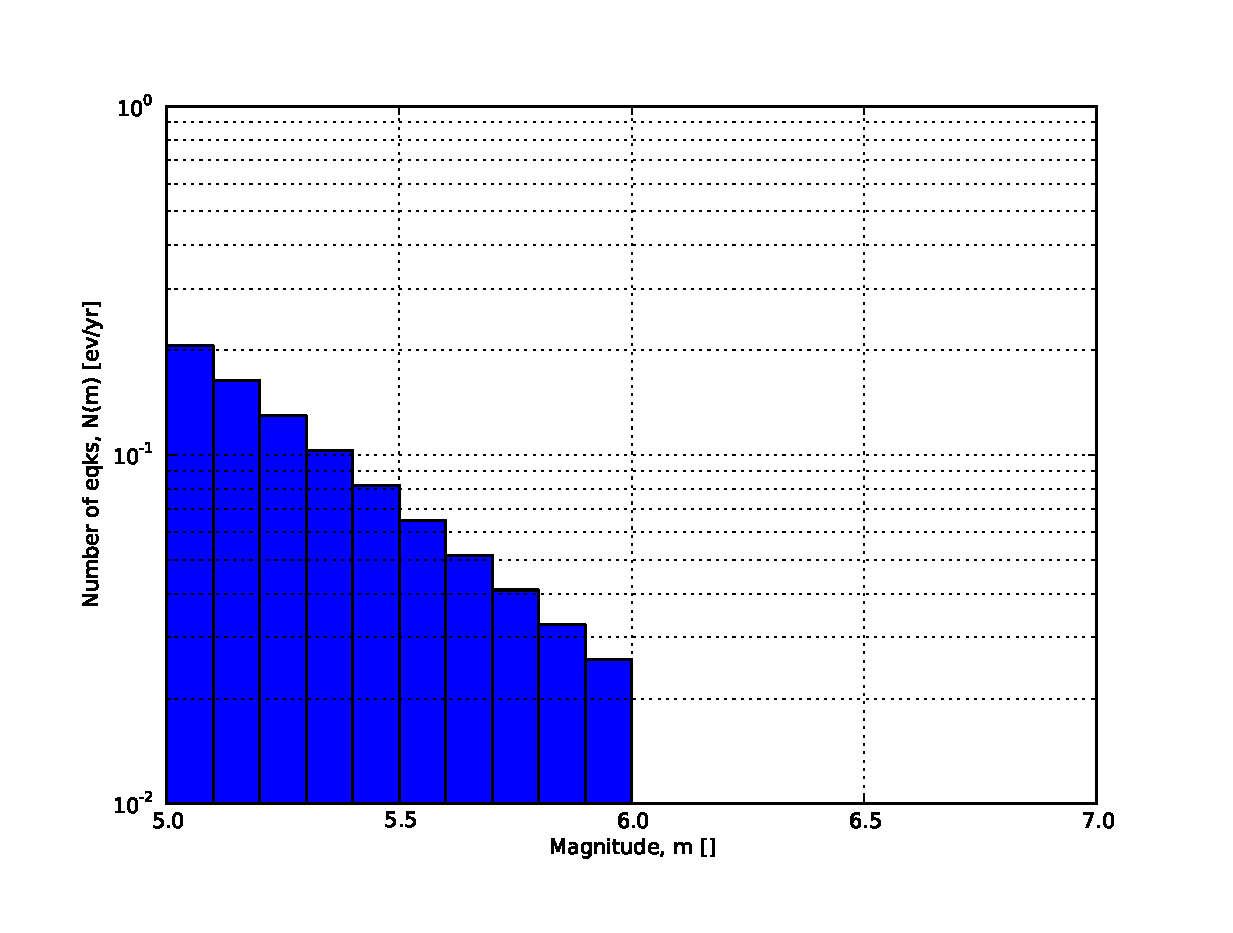
\includegraphics[width=12cm]{./figures/hazard/dt_mfd.eps}
\caption{Double truncated Gutenberg-Richter magnitude-frequency distribution.}
\label{fig:dt_gr_mfd}
\end{figure}
% . . . . . . . . . . . . . . . . . . . . . . . . . . . . . . . . . . . < Figure
% ..............................................................................
%
\item[Characteristic earthquake model (\`{a} la \cite{youngs1985})]
    The 
\begin{Verbatim}[frame=single, commandchars=\\\{\}, fontsize=\footnotesize]
    AA
\end{Verbatim}
% ..............................................................................
% . . . . . . . . . . . . . . . . . . . . . . . . . . . . . . . . . . . > Figure
\begin{figure}[!ht]
\centering
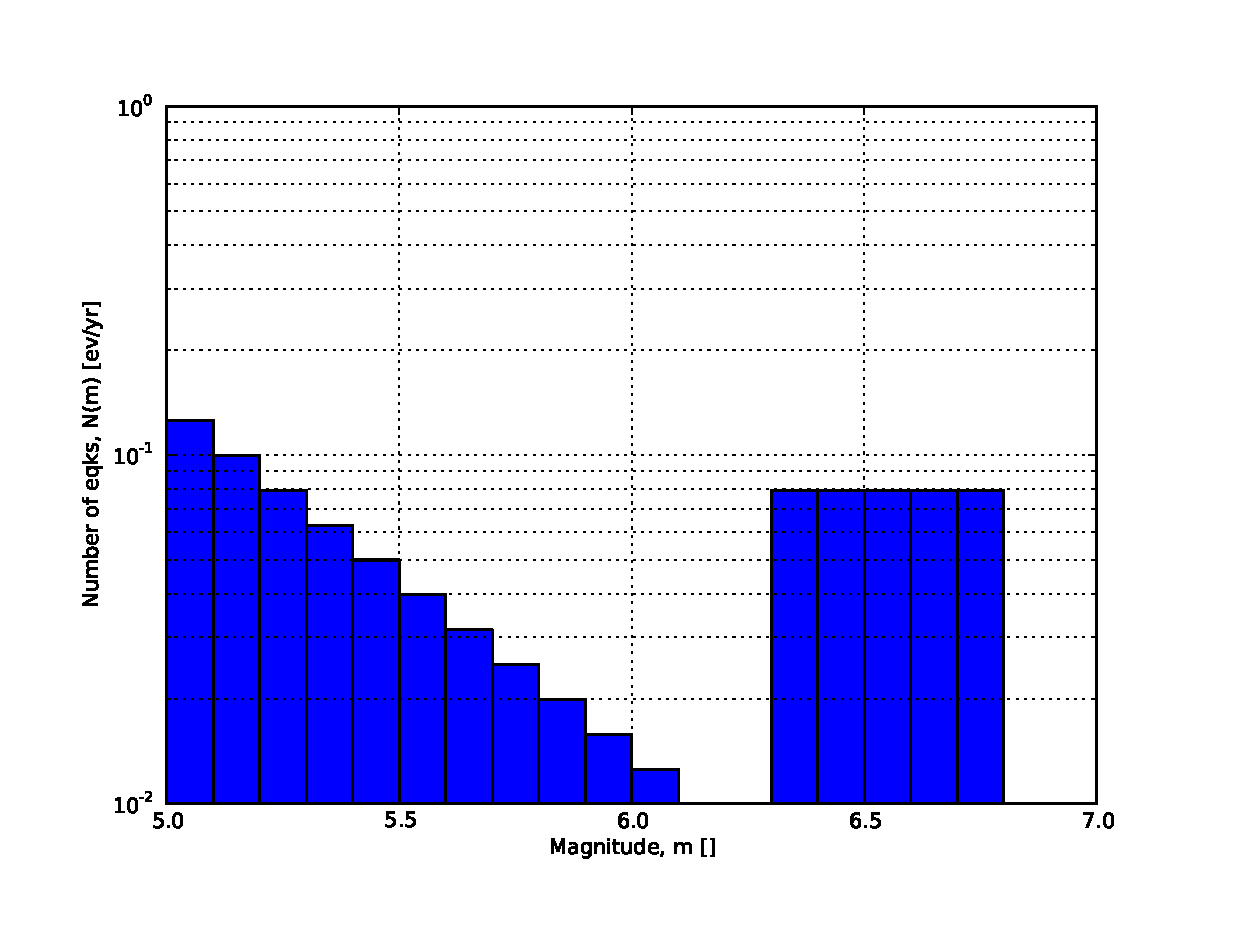
\includegraphics[width=12cm]{./figures/hazard/yc_mfd.eps}
\caption{\cite{youngs1985} magnitude-frequency distribution.}
\label{fig:yc_gr_mfd}
\end{figure}
% . . . . . . . . . . . . . . . . . . . . . . . . . . . . . . . . . . . < Figure
% ..............................................................................

\end{description}

    % -----------------------------------------------------------------------------
\section{Calculation workflows}
\index{OpenQuake-engine!Hazard calculation workflows} 
% Three types of analysis
The hazard component of the OpenQuake-engine can compute seismic hazard 
using various approaches. 
%
Three types of analysis are currently supported:
\begin{itemize}
\item \textit{Classical Probabilistic Seismic Hazard Analysis (PSHA)}, 
allowing calculation of hazard curves and hazard maps following the 
classical integration procedure 
(\cite{cornell1968}, \citet{mcguire1976}) as formulated by \cite{field2003}.
%
\item \textit{Event-Based Probabilistic Seismic Hazard Analysis}, 
    allowing calculation of ground-motion fields from 
    stochastic event sets. Traditional results - 
    such as hazard curves - can be obtained by post-processing the 
    set of computed ground-motion fields.
\item \textit{\gls{acr:ssha}}, allowing the calculation of 
    ground motion fields from a single earthquake rupture scenario 
    taking into account ground-motion aleatory variability.
\end{itemize}
%
Each workflow has a modular structure, so that intermediate results 
can be exported and analyzed. 
Each calculator can be extended independently of the others so that 
additional calculation options and methodologies can be easily 
introduced, without affecting the overall calculation workflow. 
%
%  - - - - - - - - - - - - - - - - - - - - - - - - - - - - - - - - - - - - - - -
\subsection{Classical Probabilistic Seismic Hazard Analysis}
\index{OpenQuake-engine!Hazard calculation workflows!Classical PSHA} 
\label{section:classicalPSHA}
%
Input data for the classical \gls{acr:psha} consist of a PSHA input model
provided together with calculation settings. 

The main calculators used to perform this analysis are the following:
\begin{enumerate}
\item \emph{Logic Tree Processor} \hfill \\
The Logic Tree Processor (LTP) takes as an input the \gls{acr:psha} 
Input Model and creates a Seismic Source Model. The LTP uses the 
information in the Initial Seismic Source Models and  
the Seismic Source Logic Tree to create a Seismic Source Input
Model (i.e. a model describing geometry and activity rates of each 
source without any epistemic uncertainty). 
%
Following a procedure similar to the one just described the Logic Tree 
Processor creates a Ground Motion model (i.e. a data structure that 
associates to each tectonic region considered in the calculation a 
\gls{acr:gmpe}).
%
\item \emph{Earthquake Rupture Forecast Calculator} \hfill \\
The produced Seismic Source Input Model becomes an input information for 
the Earthquake Rupture Forecast (ERF) calculator which creates a list 
earthquake ruptures admitted by the source model, each one characterized
by a probability of occurrence over a specified time span.
\item \emph{Classical PSHA Calculator} \hfill \\
The classical PSHA calculator uses the ERF and the Ground Motion model 
to compute hazard curves on each site specified in the calculation settings.
\end{enumerate} 
%
%  - - - - - - - - - - - - - - - - - - - - - - - - - - - - - - - - - - - - - - -
\subsection{Event-Based Probabilistic Seismic Hazard Analysis}
\index{OpenQuake-engine!Hazard calculation workflows!Event-based PSHA} 
\label{section:event-basedPSHA}
Input data for the Event-Based PSHA - as in the case of the 
Classical \gls{acr:psha} calculator - consist of a PSHA Input Model 
and calculation settings.

The main calculators  used to perform this analysis are:
\begin{enumerate}
%
\item \emph{Logic Tree Processor} \hfill \\
The Logic Tree Processor works in the same way described in 
the description of the Classical \gls{acr:psha} workflow 
(see section \ref{section:classicalPSHA} at page 
\pageref{section:classicalPSHA}).
%
\item \emph{Earthquake Rupture Forecast Calculator} \hfill \\ 
The Earthquake Rupture Forecast Calculator was already 
introduced in the description of the PSHA workflow (see section 
\ref{section:classicalPSHA} at page \pageref{section:classicalPSHA}).
%
\item \emph{Stochastic Event Set Calculator} \hfill \\
The Stochastic Event Set Calculator generates a collection of Stochastic 
event sets by sampling the ruptures contained in the ERF according to their 
probability of occurrence. 
%
A Stochastic Event Set (SES) thus represents a potential realisation of the 
seismicity (i.e. a list of ruptures) produced by the set of seismic sources 
considered in the analysis over the time span fixed for the 
calculation of hazard. 
%
\item \emph{Ground Motion Field Calculator} \hfill \\
The Ground Motion Field Calculator computes for each event contained in a 
Stochastic Event Set a realization of the geographic distribution of the 
shaking by taking into account the aleatory uncertainties in 
the ground-motion model. Eventually, the Ground Motion Field calculator 
can consider the spatial correlation of the ground-motion during the 
generation of the \gls{acr:gmf}.
%
\item \emph{Event-based PSHA Calculator} \hfill \\
The event-based PSHA calculator takes a (large) set of ground-motion 
fields representative of the possible shaking scenarios that the investigated
area can experience over a (long) time span and for each 
site computes the corresponding hazard curve. 
%
This procedure is computationally intensive and is not recommended for 
investigating the hazard over large areas. 
\end{enumerate}
%
%  - - - - - - - - - - - - - - - - - - - - - - - - - - - - - - - - - - - - - - -
\subsection{Scenario based Seismic Hazard Analysis}
\index{OpenQuake-engine!Hazard calculation workflows!Scenario-based SHA} 
\label{section:deterministicSHA}
In case of \gls{acr:ssha}, the input data consist of a single earthquake 
rupture model and a single ground-motion model. Using the Ground Motion Field 
Calculator, multiple realizations of ground shaking can be computed, each 
realization sampling the aleatory uncertainties in the ground-motion model.

The main calculators used to perform this analysis are:
\begin{enumerate}
\item \emph{Ground Motion Field Calculator} \hfill \\
The Ground Motion Field Calculator was already 
introduced during the description of the event based PSHA workflow (see 
section \ref{section:event-basedPSHA} at page \pageref{section:classicalPSHA}).
\end{enumerate}
% ..............................................................................
% . . . . . . . . . . . . . . . . . . . . . . . . . . . . . . . . . . . > Figure
% \begin{figure}[!hb]
% \centering
% \includegraphics[width=14cm]{./figures/deterministic_workflow.eps}
% \caption{Workflow for deterministic SHA. Given a rupture scenario model, 
% consisting of an earthquake rupture model, plus a GMPE, the ground-motion 
% field calculator can compute multiple ground-motion field realizations (by 
% taking into account GMPE aleatory uncertainties).}
% \label{deterministic_workflow}
% \end{figure}
% ..............................................................................
\cleardoublepage

\chapter{Using the hazard module}
	\label{chap:hazinp}
	This Chapter summarises the structure of the information necessary 
to define the OpenQuake-engine PSHA input model. 
% -----------------------------------------------------------------------------
% -----------------------------------------------------------------------------
\section{Input data definition}
\label{sec:hazInputData}
Input data for probabilistic based seismic hazard analysis (Classical, 
Event based, Disaggregation, and UHS) are organised into:
\begin{itemize}
\item A general configuration file;
\item A file describing the Seismic Source System, that is the set of 
    initial source models and associated epistemic uncertainties needed 
    to model the seismic activity in the region of interest.
\item A file describing the Ground Motion System, that is the set of ground 
    motion prediction equations, per tectonic region type, needed to model 
    the ground motion shaking in the region of interest.
\end{itemize}
%
Figure \ref{fig:psha_input} summarises the structure of a PSHA input model
for the OpenQuake-engine and the relationships between the files.
% ..............................................................................
% . . . . . . . . . . . . . . . . . . . . . . . . . . . . . . . . . . . > Figure
\begin{figure}[!ht]
\centering
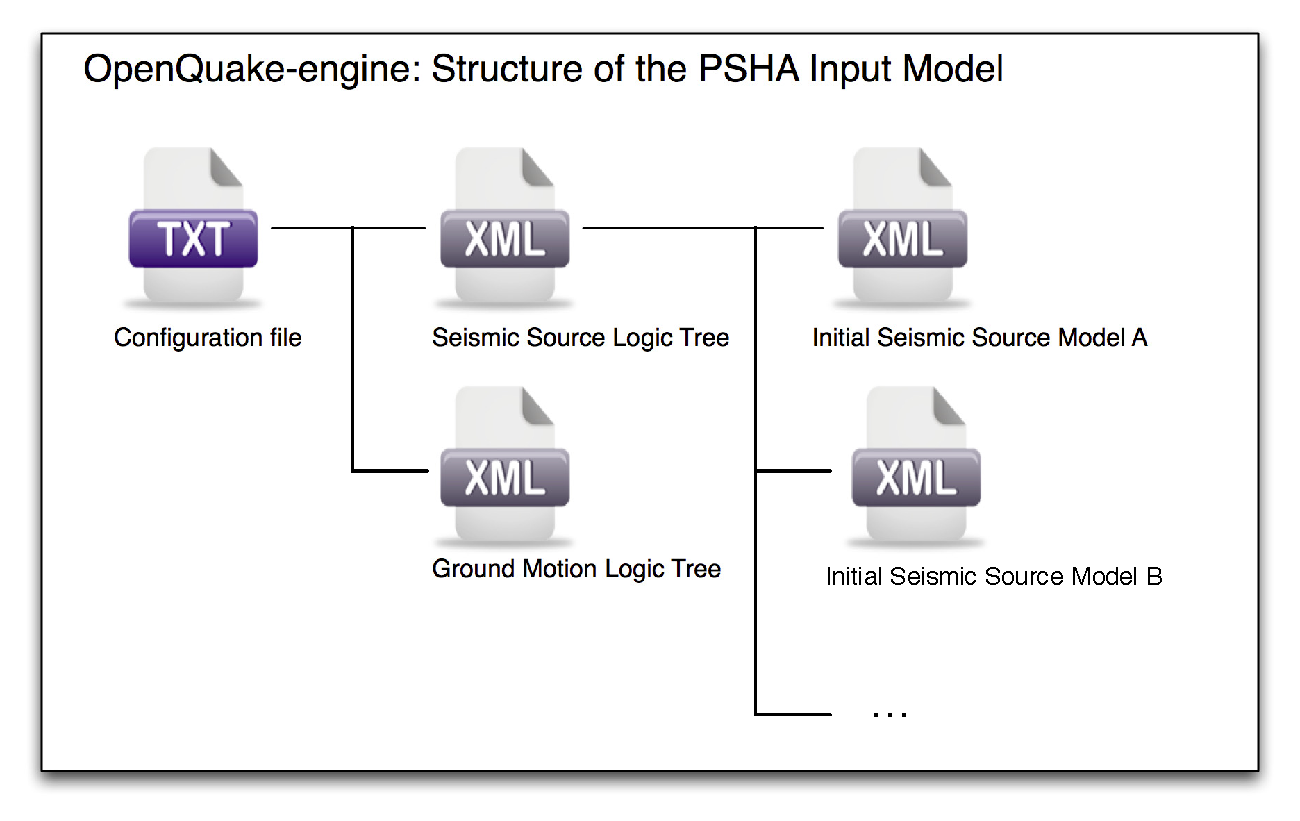
\includegraphics[width=14cm]{./figures/hazard/psha_input_structure.pdf}
\caption{PSHA Input Model structure}
\label{fig:psha_input}
\end{figure}
% . . . . . . . . . . . . . . . . . . . . . . . . . . . . . . . . . . . < Figure
% ..............................................................................
% . . . . . . . . . . . . . . . . . . . . . . . . . . . . . . . . . . . . . . .
\subsection{Defining Logic Trees in the OpenQuake engine}
The main components of a logic tree structure in the OpenQuake engine are 
the following:
\begin{description}
    \item[branch]: the simplest component of a logic tree structure. 
    A branch represents a possible interpretation/value assignment of 
    a type of uncertainty. It is fully described by the tuple 
    (parameter/model, weight).
    
    \item[branching set]: a key component in the logic tree structure 
    used by the \gls{acr:oqe}. It groups a set of branches i.e. 
    alternative interpretations of a parameter or a model. Each branching
    set is defined by:
    \begin{itemize}
        \item An ID 
        \item An uncertainty type (for a comprehensive list of the types of 
        uncertainty currently supported see Section )
        \item One or more branches
    \end{itemize}
    
    This set of uncertainties can be applied to the whole initial 
    seismic source input model or just to a subset of seismic source
    data. The sum of the weights/probabilities assigned to the set 
    of branches. 

    \item[branching level]: the largest container. It's not used in 
    modelling uncertainty, but it's useful in maintaining a logic and an 
    order in the structure of the tree.
\end{description}

Below we provide a simple schema illustrating the skeleton of the 
\gls{acr:oqe} logic tree:
\begin{Verbatim}[frame=single, commandchars=\\\{\}, fontsize=\small]
\textcolor{green}{<logicTreeBranchingLevel branchingLevelID=ID>}
    \textcolor{blue}{<logicTreeBranchSet branchSetID=ID}
            \textcolor{blue}{uncertaintyType=TYPE>}
        \textcolor{magenta}{<logicTreeBranch>}
            \textcolor{cyan}{<uncertaintyModel>VALUE</uncertaintyModel>}
            \textcolor{cyan}{<uncertaintyWeight>WEIGHT</uncertaintyWeight>}
        \textcolor{magenta}{</logicTreeBranch>}
    \textcolor{blue}{</logicTreeBranchSet>}
\textcolor{green}{</logicTreeBranchingLevel>}
\end{Verbatim}

A schematic representation of these three objects is provided in Figure 
\ref{glts}. A branching level identifies the position in a tree where
branching occurs while a branch set identifies a collection of branches 
(i.e. individual branches) whose weights sum to 1.\\
%
\begin{figure}[!h]
\centering
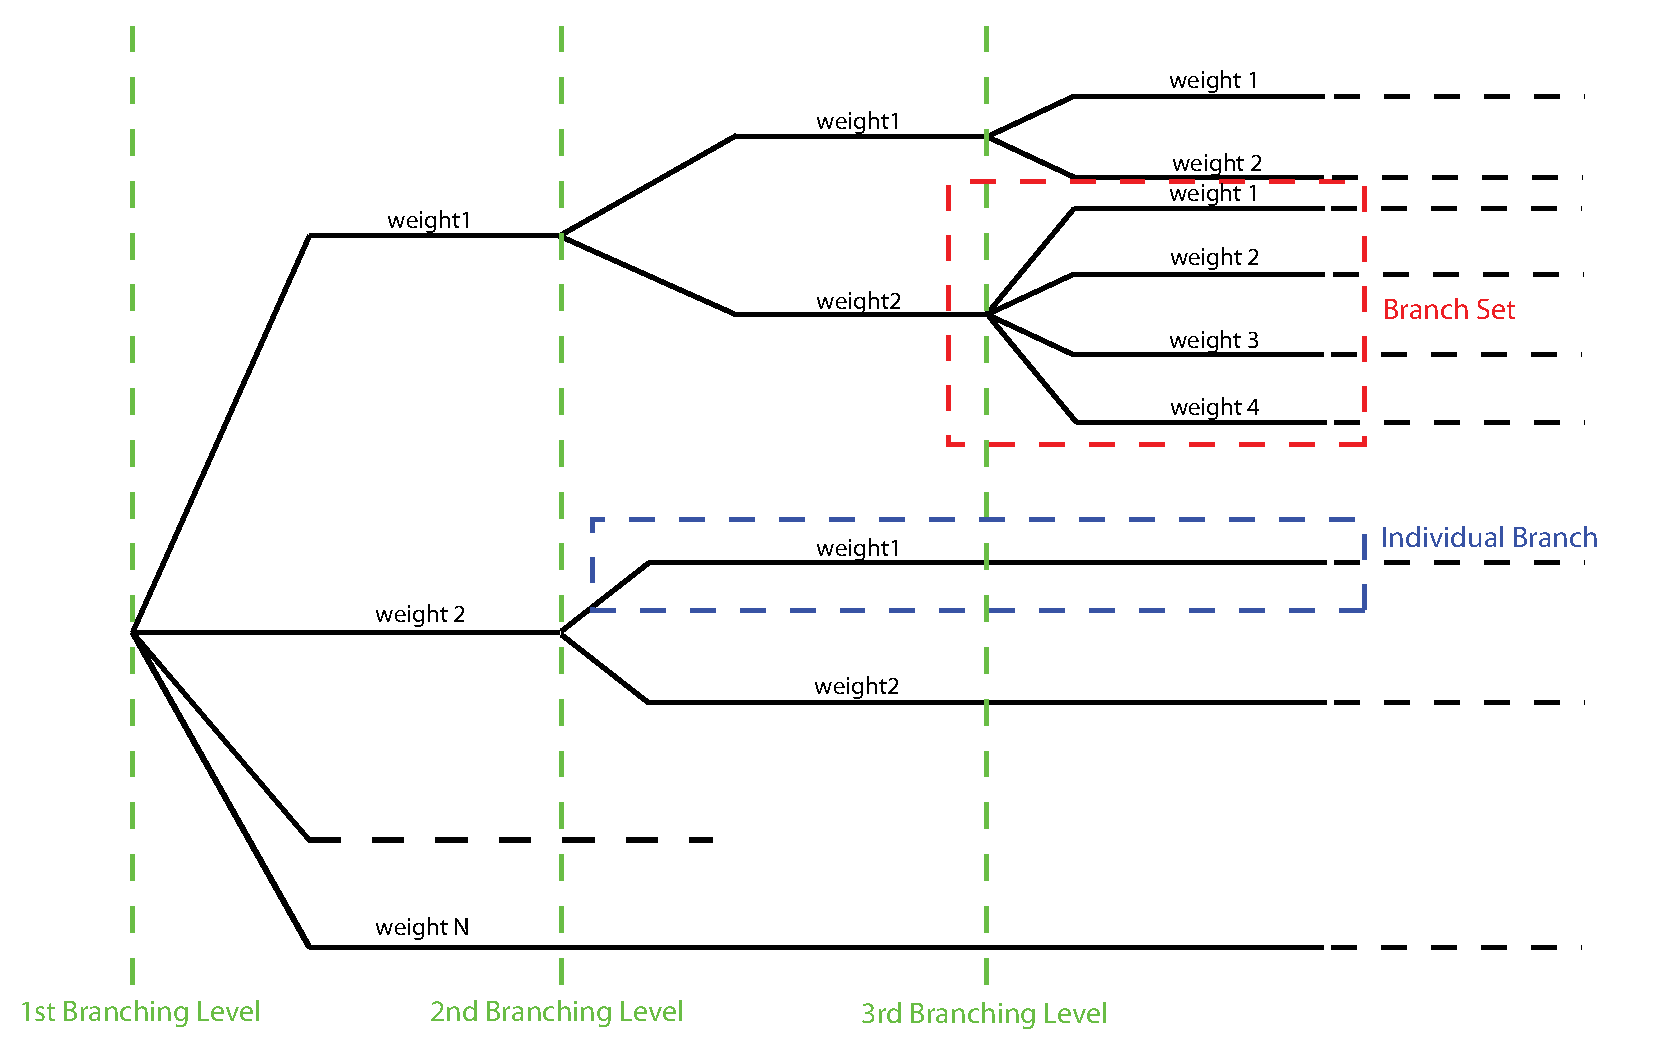
\includegraphics[width=15cm]{./figures/hazard/GenericLogicTreeStructure.eps}
\caption{Generic Logic Tree structure as described in terms of branching 
levels, branch sets, and individual branches.}
\label{glts}
\end{figure}
%
In the NRML schema, a logic tree structure is defined through the 
\Verb+logicTree+ element: 
%
\begin{Verbatim}[frame=single, commandchars=\\\{\}]
<\textcolor{red}{logicTree} logicTreeID="ID">
...
</\textcolor{red}{logicTree}>
\end{Verbatim}
%
A \Verb+logicTree+ contains as a sequence of \Verb+logicTreeBranchingLevel+ 
elements. The position in the sequence specifies in which level of the tree 
the branching level is located. That is, the first 
\texttt{logicTreeBranchingLevel} element in the sequence represents the first 
level in the tree, the second element the second level in the tree, and so on.
%
\begin{Verbatim}[frame=single, commandchars=\\\{\}]
<\textcolor{red}{logicTree} logicTreeID="ID">
	<\textcolor{green}{logicTreeBranchingLevel} branchingLevelID="ID_1">
		...
	</\textcolor{green}{logicTreeBranchingLevel}>
	<\textcolor{green}{logicTreeBranchingLevel} branchingLevelID="ID_2">
		...
	</\textcolor{green}{logicTreeBranchingLevel}>
	....
	<\textcolor{green}{logicTreeBranchingLevel} branchingLevelID="ID_N">
		...
	</\textcolor{green}{logicTreeBranchingLevel}>
</\textcolor{red}{logicTree}>
\end{Verbatim}
No restrictions are present on the number of tree levels that can 
be defined.

A \Verb+logicTreeBranchingLevel+ is defined as a sequence of 
\Verb+logicTreeBranchSet+ elements. Each \Verb+logicTreeBranchSet+ 
defines a particular epistemic uncertainty inside a branching level. 

A branch set has two required attributes (\Verb+branchSetID+ and 
\Verb+uncertaintyType+ (defining the type of epistemic uncertainty 
the branch set is defining))
\begin{Verbatim}[frame=single, commandchars=\\\{\}]
<\textcolor{red}{logicTree} logicTreeID="ID">
...
	<\textcolor{green}{logicTreeBranchingLevel} branchingLevelID="ID_#">
		<\textcolor{blue}{logicTreeBranchSet} branchSetID="ID_1"
			uncertaintyType="UNCERTAINTY_TYPE">
			...
		</\textcolor{blue}{logicTreeBranchSet}>
		<\textcolor{blue}{logicTreeBranchSet} branchSetID="ID_2"
			uncertaintyType="UNCERTAINTY_TYPE">
			...
		</\textcolor{blue}{logicTreeBranchSet}>
		...
		<\textcolor{blue}{logicTreeBranchSet} branchSetID="ID_N"
			uncertaintyType="UNCERTAINTY_TYPE">
			...
		</\textcolor{blue}{logicTreeBranchSet}>
	</\textcolor{green}{logicTreeBranchingLevel}>
...
</\textcolor{red}{logicTree}>
\end{Verbatim}
Possible values for the \Verb+uncertaintyType+ attribute are:
\begin{itemize}
\item \Verb+gmpeModel+: identifying epistemic uncertainties on ground 
motion prediction equations
\item \Verb+sourceModel+: identifying epistemic uncertainties on source models
\item \Verb+maxMagGRRelative+: identifying epistemic uncertainties 
(relative: that is increments) to be added (or subtracted, depending on 
the sign of the increment) to the 
Guten\-berg-Richter maximum magnitude value.
\item \Verb+bGRRelative+: identifying epistemic uncertainties (relative)
to be applied to the Guten\-berg-Richter b value.
\item \Verb+abGRAbsolute+:identifying epistemic uncertainties (absolute: 
that is new values used to replace original values) on the Guten\-berg-Richter
a and b values.
\item \Verb+maxMagGRAbsolute+: identifying epistemic uncertainties 
(absolute) on the Guten\-berg-Richter maximum magnitude.
\end{itemize}
No restrictions are given on the number of branch sets that can be defined 
inside a branching level.

A \Verb+branchSet+ is defined as a sequence of \Verb+logicTreeBranch+ 
elements, each specified by an \Verb+uncertaintyModel+ element (a string 
identifying an uncertainty mod\-el; the content of the string varies with
the uncertaintyType attribute value of the branchSet element) and the
uncertaintyWeight element (specifying the probability/weight associated 
to the uncertaintyModel):
\begin{Verbatim}[frame=single, commandchars=\\\{\}]
<\textcolor{red}{logicTree} logicTreeID="ID">
...
	<\textcolor{green}{logicTreeBranchingLevel} branchingLevelID="ID_#">
		...
		<\textcolor{blue}{logicTreeBranchSet} branchSetID="ID_#"
				uncertaintyType="UNCERTAINTY_TYPE">
			<\textcolor{magenta}{logicTreeBranch} branchID="ID_1">
				<uncertaintyModel>
				UNCERTAINTY_MODEL
				</uncertaintyModel>
				<uncertaintyWeight>
				UNCERTAINTY_WEIGHT
				</uncertaintyWeight>
			</\textcolor{magenta}{logicTreeBranch}>
			...
			<\textcolor{magenta}{logicTreeBranch} branchID="ID_N">
				<uncertaintyModel>
				UNCERTAINTY_MODEL
				</uncertaintyModel>
				<uncertaintyWeight>
				UNCERTAINTY_WEIGHT
				</uncertaintyWeight>
			</\textcolor{magenta}{logicTreeBranch}>
		</\textcolor{blue}{logicTreeBranchSet}>
		...
	</\textcolor{green}{logicTreeBranchingLevel}>
...
</\textcolor{red}{logicTree}>
\end{Verbatim}
Depending on the \Verb+uncertaintyType+ the content of the 
\Verb+<uncertaintyModel>+ element changes:
\begin{itemize}
\item if \Verb+uncertaintyType="gmpeModel"+, the uncertainty model 
contains the name of a ground motion prediction equation (a list of 
available GMPEs are given in appendix A), e.g.:
\begin{Verbatim}[frame=single, commandchars=\\\{\}]
<uncertaintyModel>GMPE_NAME</uncertaintyModel>
\end{Verbatim}
\item if \Verb+uncertaintyType="sourceModel"+, the uncertainty model contains 
the paths to a source model file, e.g.:
\begin{Verbatim}[frame=single, commandchars=\\\{\}]
<uncertaintyModel>SOURCE_MODEL_FILE_PATH</uncertaintyModel>
\end{Verbatim}
\item if \Verb+uncertaintyType="maxMagGRRelative"+, the uncertainty model 
contains the increment to be added (or subtracted, depending on the sign) 
to the Guten\-berg-Richter maximum magnitude:
\begin{Verbatim}[frame=single, commandchars=\\\{\}, samepage=true]
<uncertaintyModel>MAX_MAGNITUDE_INCREMENT</uncertaintyModel>
\end{Verbatim}
\item if \Verb+uncertaintyType="bGRRelative"+, the uncertainty model 
contains the increment to be added (or subtracted, depending on the 
sign) to the Guten\-berg-Richter b value:
\begin{Verbatim}[frame=single, commandchars=\\\{\}, samepage=true]
<uncertaintyModel>B_VALUE_INCREMENT</uncertaintyModel>
\end{Verbatim}
\item if \Verb+uncertaintyType="abGRAbsolute"+, the uncertainty model 
contains one (if the uncertainty apply to a source with only one 
Guten\-berg-Richter magnitude frequency distribution) or more (if the 
source has more than one magnitude frequency distributions) a and b pairs:
\begin{Verbatim}[frame=single, commandchars=\\\{\}, samepage=true]
<uncertaintyModel>
A_VALUE_1 B_VALUE_1
 ... 
A_VALUE_N B_VALUE_N
</uncertaintyModel>
\end{Verbatim}
    \item if \Verb+uncertaintyType="maxMagGRAbsolute"+, the uncertainty 
    model contains one or more (depending on the number of magnitude 
    frequency distributions in the source) Guten\-berg-Richter maximum 
    magnitude values:
%
\begin{Verbatim}[frame=single, commandchars=\\\{\}, samepage=true]
<uncertaintyModel>
MAX_MAGNITUDE_1
 ... 
MAX_MAGNITUDE_N
</uncertaintyModel>
\end{Verbatim}
\end{itemize}
%
No restrictions are given on the number of \Verb+logicTreeBranch+ elements 
that can be defined in a \Verb+logicTreeBranchSet+, as long as the uncertainty 
weights sum to 1.0.

The \Verb+logicTreeBranchSet+ element offers also a number of optional 
attributes allowing for complex tree definitions:
\begin{itemize}
    \item \Verb+applyToBranches+: specifies to which \Verb+logicTreeBranch+ 
    elements (one or more), in the previous branching level, the branch set 
    is linked to. The linking is established by defining the IDs of the 
    branches to link to:
\begin{Verbatim}[frame=single, commandchars=\\\{\}, samepage=true]
applyToBranches="branchID1 branchID2 .... branchIDN"
\end{Verbatim}
    The default is the keyword ALL, which means that a branch set is by default 
    linked to all branches in the previous branching level. By specifying one or 
    more branches to which the branch set links to, non-symmetric logic trees 
    can be defined.
    \item \Verb+applyToSources+: specifies to which source in a source model 
        the uncertainty applies to. Sources are specified in terms of their IDs:
\begin{Verbatim}[frame=single, commandchars=\\\{\}, samepage=true]
applyToSources="srcID1 srcID2 .... srcIDN"
\end{Verbatim}
    \item \Verb+applyToSourceType+: specifies to which source type the 
    uncertainty applies to.  Only one source typology can be defined 
    (\Verb+area+, \Verb+point+, \texttt{simple\-Fault}, 
	\Verb+complexFault+), e.g.:
\begin{Verbatim}[frame=single, commandchars=\\\{\}, samepage=true]
applyToSources="area"
\end{Verbatim}
    \item \Verb+applyToTectonicRegionType+: specifies to which tectonic 
    region type the uncertainty applies to. Only one tectonic region type 
    can be defined (\texttt{Ac\-tive} \texttt{Shallow Crust}, 
    \Verb+Stable Shallow Crust+, \Verb+Subduction Interface+, 
    \texttt{Sub\-duc\-tion} \texttt{IntraSlab}, \texttt{Volcanic}), e.g.:
\begin{Verbatim}[frame=single, commandchars=\\\{\}]
applyToTectonicRegionType="Active Shallow Crust"
\end{Verbatim}
\end{itemize}

% . . . . . . . . . . . . . . . . . . . . . . . . . . . . . . . . . . . . . . .
\subsection{The Seismic Source System}
The Seismic Source System contains the models describing position, geometry 
and activity of seismic sources of engineering importance for a set of sites
as well as the possible epistemic uncertainties to be incorporated into the 
calculation of seismic hazard.
%
% . . . . . . . . . . . . . . . . . . . . . . . . . . . . . . . . . . . . . . .
\subsubsection{The Seismic Source Logic Tree}
The structure of the Seismic Source Logic Tree consists of at least one 
\gls{branchinglevel}. This branching level is the one used to define the 
\gls{initialseismicsourceinputmodel} (or a number of initial seismic source 
models, see Figure \ref{fig:psha_input}). 

The example provided below shows the simplest Seismic Source Logic Tree 
structure that can be defined in a \gls{pshainputmodel} for \gls{acr:oqe}. 
This consists of a logic tree with just one branching level containing 
one \gls{branchset} with one branch used to define the initial seismic source 
model (its weight will be equal to one).
\begin{Verbatim}[frame=single, commandchars=\\\{\}, fontsize=\small,
    firstnumber=1, numbers=left, numbersep=2pt]
<?xml version="1.0" encoding="UTF-8"?>
<nrml xmlns:gml="http://www.opengis.net/gml"
      xmlns="http://openquake.org/xmlns/nrml/0.4">
    <logicTree logicTreeID="lt1">
        <logicTreeBranchingLevel branchingLevelID="bl1">
            <logicTreeBranchSet uncertaintyType="sourceModel"
                                branchSetID="bs1">
                <logicTreeBranch branchID="b1">
                    <uncertaintyModel>seismic_source_model.xml
                    </uncertaintyModel>
                    <uncertaintyWeight>1.0</uncertaintyWeight>
                </logicTreeBranch>
            </logicTreeBranchSet>
        </logicTreeBranchingLevel>
    </logicTree>
</nrml>
\end{Verbatim}

The optional branching levels will contain rules that modify parameters 
of the sources in the initial seismic source model so as to 
take into account the epistemic uncertainties. 

For example, if the principal epistemic uncertainties to be considered are
source geometry and maximum magnitude, the modeller can create a logic tree
structure with three initial seismic source models (each one exploring a 
different definition of the geometry of sources) and one branching level 
accounting for the epistemic uncertainty on the maximum magnitude.
 
Below we provide an example of such logic tree structure.
\begin{Verbatim}[frame=single, commandchars=\\\{\}, fontsize=\small,
    firstnumber=1, numbers=left, numbersep=2pt]
<?xml version="1.0" encoding="UTF-8"?>
<nrml xmlns:gml="http://www.opengis.net/gml"
      xmlns="http://openquake.org/xmlns/nrml/0.4">
    <logicTree logicTreeID="lt1">

        <logicTreeBranchingLevel branchingLevelID="bl1">
            <logicTreeBranchSet uncertaintyType="sourceModel"
                                branchSetID="bs1">
                <logicTreeBranch branchID="b1">
                    <uncertaintyModel>seismic_source_model_A.xml
                    </uncertaintyModel>
                    <uncertaintyWeight>0.2</uncertaintyWeight>
                </logicTreeBranch>
                <logicTreeBranch branchID="b2">
                    <uncertaintyModel>seismic_source_model_B.xml
                    </uncertaintyModel>
                    <uncertaintyWeight>0.3</uncertaintyWeight>
                </logicTreeBranch>
                <logicTreeBranch branchID="b3">
                    <uncertaintyModel>seismic_source_model_C.xml
                    </uncertaintyModel>
                    <uncertaintyWeight>0.5</uncertaintyWeight>
                </logicTreeBranch>
            </logicTreeBranchSet>
        </logicTreeBranchingLevel>

        <logicTreeBranchingLevel branchingLevelID="bl2">
            <logicTreeBranchSet branchSetID="bs21" 
                    uncertaintyType="maxMagGRRelative">
                <logicTreeBranch branchID="b211">
                    <uncertaintyModel>+0.0</uncertaintyModel>
                    <uncertaintyWeight>0.6</uncertaintyWeight>
                </logicTreeBranch>
                <logicTreeBranch branchID="b212">
                    <uncertaintyModel>+0.5</uncertaintyModel>
                    <uncertaintyWeight>0.4</uncertaintyWeight>
                </logicTreeBranch>
            </logicTreeBranchSet>
        </logicTreeBranchingLevel>

    </logicTree>
</nrml>
\end{Verbatim}
Note that the uncertainty on the maximum magnitude is specified in terms 
of relative increments with respect to the initial maximum magnitude 
defined for each source in the initial seismic source models.
%
% . . . . . . . . . . . . . . . . . . . . . . . . . . . . . . . . . . . . . . .
\subsubsection{The Seismic Source Model}
\index{Input!Configuration file} 
The structure of the xml file representing the seismic source 
model corresponds to a list of sources, each one modelled using 
one out of the five typologies currently supported as demonstrated in 
the following schematic example.
\begin{Verbatim}[frame=single, commandchars=\\\{\}, fontsize=\small]
<\textcolor{red}{sourceModel} gml:id="ID">
	...
	<\textcolor{green}{areaSource} gml:id="SOURCE_ID">
		<gml:name>SOURCE_NAME</gml:name>
		<tectonicRegion>TECT_REGION_TYPE</tectonicRegion>
		...
	</\textcolor{green}{areaSource}>
	...
	<\textcolor{green}{pointSource} gml:id="SOURCE_ID">
		<gml:name>SOURCE_NAME</gml:name>
		<tectonicRegion>TECT_REGION_TYPE</tectonicRegion>
		...
	</\textcolor{green}{pointSource}>
	...
	<\textcolor{green}{simpleFaultSource} gml:id="SOURCE_ID">
		<gml:name>SOURCE_NAME</gml:name>
		<tectonicRegion>TECT_REGION_TYPE</tectonicRegion>
		...
	</\textcolor{green}{simpleFaultSource}>
	...
	<\textcolor{green}{complexFaultSource} gml:id="SOURCE_ID">
		<gml:name>SOURCE_NAME</gml:name>
		<tectonicRegion>TECT_REGION_TYPE</tectonicRegion>
		...
	</\textcolor{green}{complexFaultSource}>
	...
</\textcolor{red}{sourceModel}>
\end{Verbatim}

%
% . . . . . . . . . . . . . . . . . . . . . . . . . . . . . . . . . . . . . . .
\subsection{The Ground Motion System}
\index{Input!Ground motion system} 
The Ground Motion System defines the models and possible epistemic 
uncertainties to be incorporated into the calculation of seismic hazard
and related to ground motion modelling.
%
% . . . . . . . . . . . . . . . . . . . . . . . . . . . . . . . . . . . . . . .
\subsubsection{The Ground Motion Logic Tree}
\index{Input!Ground motion logic tree} 
\label{ref:gmlt_example}
The structure of the \gls{groundmotionlogictree} consists of a list 
of ground motion prediction equations for each tectonic region used to
characterise the sources in the PSHA input model.

The example below shows a fairly simple \gls{groundmotionlogictree}. 
This logic tree assumes that all the sources in the PSHA input model 
belong to ``Active Shallow Crust'' and uses for calculation the 
\citet{chiou2008} \gls{acr:gmpe}.
\begin{Verbatim}[frame=single, commandchars=\\\{\}, fontsize=\small,
    firstnumber=1, numbers=left, numbersep=2pt]
<?xml version="1.0" encoding="UTF-8"?>
<nrml xmlns:gml="http://www.opengis.net/gml"
      xmlns="http://openquake.org/xmlns/nrml/0.4">
    <logicTree logicTreeID='lt1'>
        <logicTreeBranchingLevel branchingLevelID="bl1">
            <logicTreeBranchSet uncertaintyType="gmpeModel" 
                    branchSetID="bs1"
                    applyToTectonicRegionType="Active Shallow Crust">

                <logicTreeBranch branchID="b1">
                    <uncertaintyModel>
                    ChiouYoungs2008
                    </uncertaintyModel>
                    <uncertaintyWeight>1.0</uncertaintyWeight>
                </logicTreeBranch>

            </logicTreeBranchSet>
        </logicTreeBranchingLevel>
    </logicTree>
</nrml>
\end{Verbatim}
%
% . . . . . . . . . . . . . . . . . . . . . . . . . . . . . . . . . . . . . . . 
% . . . . . . . . . . . . . . . . . . . . . . . . . . . . . . . . . . . . . . . 
\subsection{Configuration file}
\index{Input!Configuration file} 
\label{sec:conf_file}
The configuration file is the primary file controlling both the 
definition of the input model as well as parameters governing the 
calculation. We illustrate in the following different examples of 
the configuration file addressing different typologies of seismic 
hazard calculation.
\subsubsection[Calculation of a hazard map and hazard curves using 
    classical PSHA]{Calculation of a hazard map and hazard curves using 
    the classical PSHA methodology}
\label{sec:config_classical_PSHA}
%
In the following we describe the overall structure and the
most typical parameters of a configuration file to be used for the 
computation of a seismic hazard map using a classical PSHA methodology.
\begin{itemize}
\item \textbf{Calculation type and model info}
\begin{Verbatim}[frame=single, commandchars=\\\{\}, fontsize=\small,
    numbers=left, numbersep=2pt]
[general]
description = A demo OpenQuake-engine .ini file for classical PSHA
calculation_mode = classical
random_seed = 1024
\end{Verbatim}

In this section the user specifies the following parameters:
\begin{itemize}
    \item \texttt{description}: a parameter that can be used to designate 
        the model 
    \item \texttt{calculation\_mode}: it is used to set the kind 
        of calculation. In this case it corresponds to \texttt{classical}.
        We'll describe alternative options later on.
    \item \texttt{random\_seed}: is used to control the random generator 
        so that when montecarlo procedures are used calculations are 
        replicable (if the same \texttt{random\_seed} is used).
\end{itemize}
%
\item \textbf{Geometry of the area (or the sites) where hazard is computed}
    \hfill \\
This section is used to specify where hazard will be computed. Two 
option are available. 

The first one consists on defining a polygon 
(usually a rectangle) and a distance (in km) used to discretize the 
polygon area. The polygon is defined by a list of longitude-latitude tuples.

An example is provided below.
\begin{Verbatim}[frame=single, commandchars=\\\{\}, fontsize=\small,
    firstnumber=5, numbers=left, numbersep=2pt]
[geometry]
region = 10.0 43.0, 12.0 43.0, 12.0 46.0, 10.0 46.0
\# km
region_grid_spacing = 10.0
\end{Verbatim}

The second option allows the definition of a number of sites where 
the hazard will be computed. An example is provided below.
\begin{Verbatim}[frame=single, commandchars=\\\{\}, fontsize=\small,
    firstnumber=5, numbers=left, numbersep=2pt]
[geometry]
sites = 10.0 43.0, 12.0 43.0, 12.0 46.0, 10.0 46.0
\end{Verbatim}

If the list of sites is too long the user can specify the name 
of a .csv file as it is snown below
\begin{Verbatim}[frame=single, commandchars=\\\{\}, fontsize=\small,
    firstnumber=5, numbers=left, numbersep=2pt]
[geometry]
sites\_csv = <name_of_the_csv_file>
\end{Verbatim}
%
\item \textbf{Logic tree sampling} \hfill \\
    The \gls{acr:oqe} provides two options for processing the whole 
    logic tree structure. The first option uses Montecarlo sampling;
    the user in this case specifies a number of realisations. 

    In the second option all the possible realisations are created. 
    Below we provide an example for the latter option.
    In this example we set the \texttt{number\-\_of\-\_logic\_tree\_samples}
    to 0. \gls{acr:oqe} will perform a complete enumeration of all 
    the possible paths from the roots to the leaves of the logic tree 
    structure.
\begin{Verbatim}[frame=single, commandchars=\\\{\}, fontsize=\small,
    firstnumber=9, numbers=left, numbersep=2pt]
[logic_tree]
number_of_logic_tree_samples = 0
\end{Verbatim}
    If the seismic source logic tree and the ground motion
    logic tree do not contain epistemic uncertainties the engine will
    create a single PSHA input.
%
\item \textbf{Parameters controlling the construction of the earthquake 
    rupture forecast}
\begin{Verbatim}[frame=single, commandchars=\\\{\}, fontsize=\small,
    firstnumber=11, numbers=left, numbersep=2pt]
[erf]
# km
rupture_mesh_spacing = 5
width_of_mfd_bin = 0.1
# km
area_source_discretization = 10
\end{Verbatim}
This section of the configuration file is used to specify the 
level of discretization of the mesh representing faults, of the grid
used to delineate the area sources and, of the magnitude-frequency 
distribution. 
Note that the lower is the mesh spacing (or the bin width) the higher 
are the precision in the representation and the computation demand.
%
\item \textbf{Parameters describing site conditions}
\begin{Verbatim}[frame=single, commandchars=\\\{\}, fontsize=\small,
    firstnumber=17, numbers=left, numbersep=2pt]
[site_params]
reference_vs30_type = measured
reference_vs30_value = 760.0
reference_depth_to_2pt5km_per_sec = 5.0
reference_depth_to_1pt0km_per_sec = 100.0
\end{Verbatim}
In this section the user specifies local soil conditions. The simplest
solution is to define uniform site conditions (i.e. all the sites have 
the same soil conditions). Alternatively it's possible to define 
spatially variable soil properties in a separate file; the engine will
then assign to each investigation site the appropriate characteristics.
%
\begin{Verbatim}[frame=single, commandchars=\\\{\}, fontsize=\small,
    firstnumber=17, numbers=left, numbersep=2pt]
[site_params]
site_model_file = ../_site_model/site_model.xml
\end{Verbatim}

The file containing the site model has the following 
structure:
\begin{Verbatim}[frame=single, commandchars=\\\{\}, fontsize=\small]
<?xml version="1.0" encoding="utf-8"?>
<nrml xmlns:gml="http://www.opengis.net/gml"
      xmlns="http://openquake.org/xmlns/nrml/0.4">
    <siteModel>
        <site lon="10.0" lat="40.0" vs30="800.0" 
            vs30Type="inferred" 
            z1pt0="19.367196734" z2pt5="0.588625072259" />
        <site lon="10.1" lat="40.0" vs30="800.0" 
            vs30Type="inferred" 
            z1pt0="19.367196734" z2pt5="0.588625072259" />
        <site lon="10.2" lat="40.0" vs30="800.0" 
            vs30Type="inferred" 
            z1pt0="19.367196734" z2pt5="0.588625072259" />
        <site lon="10.3" lat="40.0" vs30="800.0" 
            vs30Type="inferred" 
            z1pt0="19.367196734" z2pt5="0.588625072259" />
        <site lon="10.4" lat="40.0" vs30="800.0" 
            vs30Type="inferred" 
            z1pt0="19.367196734" z2pt5="0.588625072259" />
        ...
    </siteModel>
</nrml>
\end{Verbatim}

%
\item \textbf{Calculation configuration}
\phantomsection
\label{sec:calculation_configuration}
\begin{Verbatim}[frame=single, commandchars=\\\{\}, fontsize=\small,
     firstnumber=22, numbers=left, numbersep=2pt]
[calculation]
source_model_logic_tree_file = source_model_logic_tree.xml
gsim_logic_tree_file = gmpe_logic_tree.xml
# years
investigation_time = 50.0
intensity_measure_types_and_levels = \{"PGA": [0.005, ..., 2.13]\} 
truncation_level = 3
# km
maximum_distance = 200.0
\end{Verbatim}
This section of the \gls{acr:oqe} configuration file specifies the 
parameters that
are relevant for the calculation of hazard. These include the names of
the two files containing the Seismic Source System and the Ground 
Motion System, the duration of the time window used to compute the 
hazard, the ground motion intensity measure types and levels for 
which the probability of exceedence will be computed, the level of
truncation of the gaussian 
distribution of the logarithm of ground motion used in the calculation 
of hazard and the maximum integration distance (i.e. the distance within 
which sources will contribute to the computation of the hazard).
%
\item \textbf{Output}
\begin{Verbatim}[frame=single, commandchars=\\\{\}, fontsize=\small,
    firstnumber=32, numbers=left, numbersep=2pt]
[output]
export_dir = out/
# given the specified `intensity_measure_types_and_levels`
quantile_hazard_curves =
poes_hazard_maps = 0.1
\end{Verbatim}
The final section of the configuration file is the one that contains 
the parameters controlling the typology of output to be produced.
%
\end{itemize}
%
%\input{config_file_event_based.tex}
%

\subsubsection{Seismic hazard disaggregation}
%
In this section we describe the structure of the configutation 
file to be used to complete a seismic hazard disaggregation. 
Since only a few parts of the standard configuration file need to 
be changed we'll use the description given in Section 
\ref{sec:config_classical_PSHA} at page 
\pageref{sec:config_classical_PSHA} as a reference and we'll 
emphasize in the following major differences.
%
\begin{itemize}
%
\item \textbf{Calculation type and model info}
\begin{Verbatim}[frame=single, commandchars=\\\{\}, fontsize=\small]
[general]
description = A demo .ini file for PSHA disaggregation
calculation_mode = disaggregation
random_seed = 1024
\end{Verbatim}
The calculation mode parameter in this case is set as 
\texttt{disaggregation}.
%
\item \textbf{Geometry of the area (or the sites) where hazard is computed}
\begin{Verbatim}[frame=single, commandchars=\\\{\}, fontsize=\small]
[geometry]
sites = 11.0 44.5


\end{Verbatim}
In the section it will be necessary to specify the geographic 
coordinates of the site (or the sites) where the disaggregation
will be performed.
%
\item \textbf{Disaggregation parameters}
\begin{Verbatim}[frame=single, commandchars=\\\{\}, fontsize=\small]
[disaggregation]
poes_disagg = 0.02, 0.1
mag_bin_width = 1.0
distance_bin_width = 25.0
# decimal degrees
coordinate_bin_width = 1.5
num_epsilon_bins = 3
\end{Verbatim}
With the disaggregation settings shown above we'll disaggregate the intensity
measure levels with 10\% and 2\% probability of exceedance using the
\texttt{in\-ves\-ti\-gation\_time} and the intensity measure types 
defined in the ``Calculation configuration'' section of the OpenQuake
configuration file (see page \pageref{sec:calculation_configuration}). 
\end{itemize}

\subsubsection{Event based PSHA}
%
In the following we describe the sections of the configuration file 
that are required to complete event based PSHA calculations 
\begin{enumerate}
\item \textbf{Calculation type and model info} \hfill \\
    This part is almost identical to the corresponding one 
    described in section \ref{sec:config_classical_PSHA}. Note
    the setting of the \texttt{cal\-cu\-lation\_mode} parameter
    which now corresponds to \texttt{event\_based}.
\begin{Verbatim}[frame=single, commandchars=\\\{\}, fontsize=\small,
    numbers=left, numbersep=2pt]
[general]
description = A demo OpenQuake-engine .ini file for classical PSHA
calculation_mode = event_based
random_seed = 1024
\end{Verbatim}
%
\item \textbf{Event based} \hfill \\
This is section is used to specify the number of stochastic 
event sets to be generated for each logic tree realisation 
(each stochastic event set represents a potential realisation of seismicity
during the \texttt{in\-ves\-ti\-gation\_time} specified in the 
\texttt{calculation\_configuration} part).
Additionally, in this section the user can specify the spatial correlation
model to be used in case for the generation of ground motion fields. 
\begin{Verbatim}[frame=single, commandchars=\\\{\}, fontsize=\small]
[event_based_params]
ses_per_logic_tree_path = 5
ground_motion_correlation_model = JB2009
ground_motion_correlation_params = {"vs30_clustering": true}
\end{Verbatim}
%
\item \textbf{Output} \hfill \\
This part substitutes the \texttt{Output} part described in 
the configuration file example described in the section 
\ref{sec:config_classical_PSHA}
at page \pageref{sec:config_classical_PSHA}.
\begin{Verbatim}[frame=single, commandchars=\\\{\}, fontsize=\small]
[output]
export_dir = /tmp/xxx
complete_logic_tree_ses = true
complete_logic_tree_gmf = true
ground_motion_fields = true
# post-process ground motion fields into hazard curves,
# given the specified `intensity_measure_types_and_levels`
hazard_curves_from_gmfs = true
mean_hazard_curves = true
quantile_hazard_curves = 0.15, 0.5, 0.85
poes_hazard_maps = 0.1, 0.2
\end{Verbatim}
%
\end{enumerate}


\chapter{Hazard calculation and results provided}
	\label{chap:hazout}
	In this Chapter we provide a desciption of the main commands available
for running hazard with the \gls{acr:oqe} and the file formats used to 
represent the results of the analyses.

A general introduction to the use of OpenQuake is provided in Section 
\ref{sec:intro} at page \pageref{sec:intro}.
The reader is invited to consult this part before moving into
the details of this section.
% -----------------------------------------------------------------------------
\section{Running OpenQuake-engine for hazard calculations}
\index{Running OpenQuake!hazard} 
The execution of a hazard analysis using the OpenQuake-engine 
is straightforward. Below we provide an example of the simplest 
command that can be used to launch a hazard calculation which 
consists in the invocation of \texttt{openquake} together with 
the \texttt{--rh} option which stands for ``run hazard'' and 
the name of a configuration file (in the example below
it corresponds to \texttt{job.ini}):
\begin{Verbatim}[frame=single, commandchars=\\\{\}, fontsize=\small]
user@ubuntu:~$ oq-engine --rh job.ini
\end{Verbatim}

The amount of information prompted during the execution of the 
analysis is controlled by means of the \texttt{--log-level} flag 
as shown in the example below:
\begin{Verbatim}[frame=single, commandchars=\\\{\}, fontsize=\small]
user@ubuntu:~$ oq-engine --rh job.ini --log-level debug
\end{Verbatim}
In this example we ask the engine to provide an extensive amount
of information (usually not justified for a standard analysis). 
Alternative options are: \texttt{debug}, \texttt{info}, \texttt{progress},
\texttt{warn}, \texttt{error}, \texttt{critical}.
% -----------------------------------------------------------------------------
\subsection{Getting results}
\label{sec:getting_results}
There are two alternative ways to get results from the OpenQuake engine:
directly through the calculation or by exporting them from the 
internal \gls{acr:oqe} database once a calculation is completed. 

The first option is activated at the OpenQuake engine invocation by 
the flag \texttt{--exports xml} as shown in the example below
\begin{Verbatim}[frame=single, commandchars=\\\{\}, fontsize=\small]
user@ubuntu:~$ oq-engine --rh job.ini \textcolor{red}{--exports xml}
\end{Verbatim}

The second option, allows the user to export the computed results at 
their's disposal.
In order to get the list of results of the hazard calculations stored 
in the \gls{acr:oqe} database the user can utilize the following command:
\begin{Verbatim}[frame=single, commandchars=\\\{\}, fontsize=\small]
user@ubuntu:~$ oq-engine --lhc
\end{Verbatim}
The execution of this command will produce a list similar to the 
one provided below (the numbers in red are the calculations IDs).
\begin{Verbatim}[frame=single, commandchars=\\\{\}, fontsize=\small]
user@ubuntu:~$ oq-engine --lhc
calc_id | num_jobs | latest_job_status | last_update | description
\textcolor{red}{1} | 1 | failed | 2013-03-01 09:49:34  | Classical PSHA
\textcolor{red}{2} | 1 | successful | 2013-03-01 09:49:56  | Classical PSHA
\textcolor{red}{3} | 1 | failed | 2013-03-01 10:24:04  | Classical PSHA
\textcolor{red}{4} | 1 | failed | 2013-03-01 10:28:16  | Classical PSHA
\textcolor{red}{5} | 1 | failed | 2013-03-01 10:30:04  | Classical PSHA
\textcolor{red}{6} | 1 | successful | 2013-03-01 10:31:53  | Classical PSHA
\textcolor{red}{7} | 1 | failed | 2013-03-09 08:15:14  | Classical PSHA
\textcolor{red}{8} | 1 | successful | 2013-03-09 08:18:04  | Classical PSHA
\end{Verbatim}
Subsequently the user can get the list of result stored for a specific 
hazard analysis as in the example below (note that the number in blue 
emphasizes the result ID)
\begin{Verbatim}[frame=single, commandchars=\\\{\}, fontsize=\small]
user@ubuntu:~$ oq-engine --lho <calc_id>
id | output_type | name
\textcolor{blue}{3} | hazard_curve | hc-rlz-6
\end{Verbatim}
and finally extract an xml file for a specific hazard result 
\begin{Verbatim}[frame=single, commandchars=\\\{\}, fontsize=\small]
user@ubuntu:~$ oq-engine --eh <result_id> <path_to_the_output_folder>
\end{Verbatim}
% -----------------------------------------------------------------------------
% -----------------------------------------------------------------------------
\section{Description of outputs}
The results generated by the OpenQuake-engine are fundamentally 
of two distinct typologies differentiated by the presence (or 
absence) of epistemic uncertainty in the PSHA input model.

When epistemic uncertainty is incorporated into the 
calculation, the Open\-Quake\--engine calculators (e.g. Classical 
PSHA, Event Based PSHA, Disaggregation, UHS) produce a 
'distribution' of results (hazard curves, ground motion fields, 
disaggregation matrices, UHS) which is specular to the epistemic 
uncertainties introduced in the PSHA input model.

For each logic tree sample, results are computed and stored. 
Calculation of results statistics (mean, standard deviation, 
quantiles) are included in the hazard module of the 
OpenQuake-engine calculators (the only exception being 
disaggregation).
% - - - - - - - - - - - - - - - - - - - - - - - - - - - - - - - - - - - - - - -
\subsection{Output from Classical PSHA}
By default, the classical PSHA calculator computes and stores 
hazard curves for each logic tree sample considered.

When the PSHA input model doesn't contain epistemic uncertainties
the results will consist on a set of hazard curves (one for each 
investigated site). 
The command below illustrates how is possible to retrieve the group
of hazard curves obtained for a calcualtion with a given calculation
identifies \texttt{<calc\_id>}:
\begin{Verbatim}[frame=single, commandchars=\\\{\}, fontsize=\small]
user@ubuntu:~$ openquake --lho <calc_id>
id | output_type | name
\textcolor{red}{3 | hazard_curve | hc-rlz-6}
\end{Verbatim}
In this case \gls{acr:oqe} produced a group of hazard curves with 
identifier \texttt{3}.
% 
On the contrary, if \texttt{number\_of\_logic\_tree\_samples}, 
N hazard curves files are generated:
\begin{Verbatim}[frame=single, commandchars=\\\{\}, fontsize=\small]
user@ubuntu:~$ openquake --lho <calc_id>
id | output_type | name
\textcolor{red}{5 | hazard_curve | hc-rlz-10}
\textcolor{red}{6 | hazard_curve | hc-rlz-7}
\textcolor{red}{7 | hazard_curve | hc-rlz-8}
\textcolor{red}{8 | hazard_curve | hc-rlz-9}
\textcolor{red}{9 | hazard_curve | hc-rlz-11}
\textcolor{red}{10 | hazard_curve | hc-rlz-12}
\end{Verbatim}
If we export from the database the hazard curves contained in 
one of the items above through the following command
\begin{Verbatim}[frame=single, commandchars=\\\{\}, fontsize=\small]
user@ubuntu:~$ openquake --eh <output_id> <output_directory>
\end{Verbatim}
we will obtain a nrml formatted file as represented in the example
in the inset \ref{vrb:haz_curves}.
\begin{nrmlsmp}
\begin{Verbatim}[frame=single, commandchars=\\\{\}, fontsize=\small]
<?xml version='1.0' encoding='UTF-8'?>
<nrml xmlns:gml="http://www.opengis.net/gml" 
      xmlns="http://openquake.org/xmlns/nrml/0.4">
  <hazardCurves \textcolor{red}{sourceModelTreePath="b1|b212"} 
      \textcolor{red}{gsimTreePath="b2" IMT="PGA" investigationTime="50.0"}>
    \textcolor{green}{<IMLs>0.005 0.007 0.0098 ... 1.09 1.52 2.13</IMLs>}
    <hazardCurve>
      <gml:Point>
      \textcolor{blue}{<gml:pos>10.0 45.0</gml:pos>}
      </gml:Point>
      <poEs>1.0 1.0 1.0 ... 0.000688359310522 0.0 0.0</poEs>
    </hazardCurve>
    ...
    <hazardCurve>
      <gml:Point>
      \textcolor{blue}{<gml:pos>lon lat</gml:pos>}
      </gml:Point>
      <poEs>poe1 poe2 ... poeN</poEs>
    </hazardCurve>
  </hazardCurves>
</nrml>
\end{Verbatim}
\caption{Hazard curves: nrml sample file}
\label{vrb:haz_curves}
\end{nrmlsmp}
Not\-with\-stand\-ing the intuitiveness of this file, let's have a brief 
overview of the information included.

The overall content of this file is a list of hazard curves, one for
each investigated site, computed using a PSHA input model which 
can be either the single PSHA input model (if epistemic 
uncertainties are not accounted) or one possible realisation of 
the complete logic tree structure. In the current example these 
hazard curves corresponds to one of a set of results produced to 
account for epistemic uncertainties.

The attributes of the \texttt{hazardCurves} element (see text in 
red in the example above) specify the path in the logic tree 
used to create the seismic source model (\texttt{source\-Model\-TreePath}) 
and the ground motion model (\texttt{gsim\-Tree\-Path}) plus the 
intensity measure type and the investigation time used to compute 
the probability of exceedance. 

The \texttt{IMLs} element (in green in the example above) contains the 
values of shaking for which the engine computed the probability of 
exceedance in the investigation time.
For each site this file contains a \texttt{hazardCurve} element which 
includes the coordinates (longitude and latitude in decimal degrees) 
of the site and the values of the probability of exceedance for all the 
intensity measure levels specified in the \texttt{IMLs} element.

If in the configuration file the calculation of mean hazard curves 
and hazard curves corresponding to one or several percentiles have 
been specified, the list of outputs we should expect from OpenQuake 
corresponds to:
\begin{Verbatim}[frame=single, commandchars=\\\{\}, fontsize=\small]
user@ubuntu:~$ openquake --lho <calc_id> 
id | output_type | name
17 | hazard_curve | hc-rlz-17
18 | hazard_curve | hc-rlz-18
19 | hazard_curve | hc-rlz-13
20 | hazard_curve | hc-rlz-14
21 | hazard_curve | hc-rlz-15
22 | hazard_curve | hc-rlz-16
\textcolor{red}{23 | hazard_curve | quantile(0.5)-curves-PGA}
24 | hazard_map | hazard-map(0.1)-PGA-rlz-17
25 | hazard_map | hazard-map(0.1)-PGA-rlz-18
26 | hazard_map | hazard-map(0.1)-PGA-rlz-13
27 | hazard_map | hazard-map(0.1)-PGA-rlz-14
28 | hazard_map | hazard-map(0.1)-PGA-rlz-15
29 | hazard_map | hazard-map(0.1)-PGA-rlz-16
\textcolor{red}{30 | hazard_map | hazard-map(0.1)-PGA-quantile(0.5)}
\end{Verbatim}
In this example \gls{acr:oqe} produced hazard curves and hazard maps for 
six logic tree realisations plus median hazard curves (highlited in red)
and median hazard map (also highlighted in red).

In the inset \ref{vrb:haz_map} we show a sample nrml file used 
to describe a hazard map.
\begin{nrmlsmp}
\begin{Verbatim}[frame=single, commandchars=\\\{\}, fontsize=\small]
<?xml version='1.0' encoding='UTF-8'?>
<nrml xmlns:gml="http://www.opengis.net/gml" 
      xmlns="http://openquake.org/xmlns/nrml/0.4">
  \textcolor{red}{<hazardMap sourceModelTreePath="b1" gsimTreePath="b1"}
        \textcolor{red}{IMT="PGA" investigationTime="50.0" poE="0.1">}
    <node lon="119.596690957" lat="21.5497682591" iml="0.204569990197"/>
    <node lon="119.596751048" lat="21.6397004197" iml="0.212391638188"/>
    <node lon="119.596811453" lat="21.7296325803" iml="0.221407505615"/>
    ...
  </hazardMap>
</nrml>
\end{Verbatim}
\caption{Hazard map: nrml sample file}
\label{vrb:haz_map}
\end{nrmlsmp}

\section{Output from Event Based PSHA}\label{EventBasedOutput}
%
The Event Based PSHA calculator computes and stores stochastic 
event sets and the corresponding ground motion fields. In case,
this calculator can also compute hazard curves and hazard maps
exactly in the same way is done using the Classical PSHA calculator.

The inset below shows an example of the list of results provided by 
\gls{acr:oqe} at the end of an event-based PSHA calculation:
%
\begin{Verbatim}[frame=single, commandchars=\\\{\}, fontsize=\small]
user@ubuntu:~$ oq-engine --lho <calc_id> 
id | output_type | name
\textcolor{red}{31 | ses | ses-coll-rlz-19}
\textcolor{green}{32 | gmf | gmf-rlz-19}
\textcolor{red}{33 | ses | ses-coll-rlz-20}
\textcolor{green}{34 | gmf | gmf-rlz-20}
35 | hazard_curve | hazard-curve-rlz-19-SA(0.1)
36 | hazard_curve | hazard-curve-rlz-20-SA(0.1)
37 | hazard_curve | hazard-curve-rlz-19-PGA
38 | hazard_curve | hazard-curve-rlz-20-PGA
39 | hazard_curve | mean curve for SA(0.1)
40 | hazard_curve | quantile curve (poe >= 0.15) for imt SA(0.1)
41 | hazard_curve | quantile curve (poe >= 0.5) for imt SA(0.1)
42 | hazard_curve | quantile curve (poe >= 0.85) for imt SA(0.1)
43 | hazard_curve | mean curve for PGA
44 | hazard_curve | quantile curve (poe >= 0.15) for imt PGA
45 | hazard_curve | quantile curve (poe >= 0.5) for imt PGA
46 | hazard_curve | quantile curve (poe >= 0.85) for imt PGA
\end{Verbatim}
This list contains two sets of stochastic events (in red) two sets of ground motion fields (in blue).

The whole group of stochastic event set and ground motion fields can 
be exported immediately using the results with \texttt{id} 35 and 25,
respectively.

In the remaining part of this Section we show an example of a file
containing a stochastic event set and a file containing a ground 
motion field.

This is an example showing a nrml file containing two a collection of 
stochastic event sets 
\begin{Verbatim}[frame=single, commandchars=\\\{\}, fontsize=\small]
<?xml version='1.0' encoding='UTF-8'?>
<nrml xmlns:gml="http://www.opengis.net/gml" 
	  xmlns="http://openquake.org/xmlns/nrml/0.4">
  <stochasticEventSetCollection sourceModelTreePath="b1" 
          gsimTreePath="b1">
    \textcolor{red}{<stochasticEventSet id="12" investigationTime="50.0">}
      <rupture id="533" magnitude="4.55" strike="90.0" dip="90.0" 
              rake="90.0" tectonicRegion="Active Shallow Crust">
        <planarSurface>
          <topLeft lon="12.233903801" lat="43.256198599" 
                  depth="11.3933265259"/>
          <topRight lon="12.263958243" lat="43.2562025344" 
                  depth="11.3933265259"/>
          <bottomLeft lon="12.233903801" lat="43.256198599" 
                  depth="12.6066734741"/>
          <bottomRight lon="12.263958243" lat="43.2562025344" 
                  depth="12.6066734741"/>
        </planarSurface>
      </rupture>
      <rupture id="535" magnitude="4.65" strike="135.0" dip="90.0" 
              rake="90.0" tectonicRegion="Active Shallow Crust">
        <planarSurface>
          <topLeft lon="11.45858812" lat="42.7429056814" 
                  depth="11.3208667302"/>
          <topRight lon="11.4822820715" lat="42.7256333907" 
                  depth="11.3208667302"/>
          <bottomLeft lon="11.45858812" lat="42.7429056814" 
                  depth="12.6791332698"/>
          <bottomRight lon="11.4822820715" lat="42.7256333907" 
                  depth="12.6791332698"/>
        </planarSurface>
      </rupture>
    \textcolor{red}{</stochasticEventSet>}
  </stochasticEventSetCollection>
</nrml>
\end{Verbatim}
This is an example showing a nrml file containing a collection of
ground motion fields:
\begin{Verbatim}[frame=single, commandchars=\\\{\}, fontsize=\small]
<?xml version='1.0' encoding='UTF-8'?>
<nrml xmlns:gml="http://www.opengis.net/gml" 
      xmlns="http://openquake.org/xmlns/nrml/0.4">
  <gmfCollection sourceModelTreePath="b1" gsimTreePath="b1">
    <gmfSet investigationTime="50.0" stochasticEventSetId="12">
      <gmf IMT="PGA" ruptureId="533">
        <node gmv="0.0105891230432" lon="11.1240023202" 
            lat="43.5107462335"/>
        <node gmv="0.00905803920023" lon="11.1241875202" 
            lat="43.6006783941"/>
        <node gmv="0.00637664420977" lon="11.124373581" 
            lat="43.6906105547"/>
        <node gmv="0.00476533134789" lon="11.1245605075" 
            lat="43.7805427153"/>
        <node gmv="0.00452594698469" lon="11.1247483046" 
            lat="43.8704748759"/>
        ...
        <node gmv="0.000173010769646" lon="11.3782630185" 
            lat="44.5"/>
      </gmf>
    </gmfSet>
  </gmfCollection>
</nrml>
\end{Verbatim}

\section{Output from Disaggregation}
The output from an \gls{acr:oqe} disaggregation analysis  
correspond to the combination of a hazard curve and a multidimensional 
matrix containing the results of the disaggregation.

The example below shows the list of disaggregation results obtained 
for four logic tree realisations. 
For each realisation, disaggregation has been completed for two  
intensity measure levels corresponding to different probabilities of 
exceedence in the specified \texttt{investigation time}.
\begin{Verbatim}[frame=single, commandchars=\\\{\}, samepage=true]
user@ubuntu:~$ openquake --lho <calc_id> 
id | output_type | name
19 | hazard_curve | hc-rlz-3
20 | hazard_curve | hc-rlz-3
21 | hazard_curve | hc-rlz-4
22 | hazard_curve | hc-rlz-4
23 | disagg_matrix | disagg(0.02)-rlz-3-SA(0.025)-POINT(10.1 40.1)
24 | disagg_matrix | disagg(0.1)-rlz-3-SA(0.025)-POINT(10.1 40.1)
25 | disagg_matrix | disagg(0.02)-rlz-3-PGA-POINT(10.1 40.1)
26 | disagg_matrix | disagg(0.1)-rlz-3-PGA-POINT(10.1 40.1)
27 | disagg_matrix | disagg(0.02)-rlz-4-SA(0.025)-POINT(10.1 40.1)
28 | disagg_matrix | disagg(0.1)-rlz-4-SA(0.025)-POINT(10.1 40.1)
29 | disagg_matrix | disagg(0.02)-rlz-4-PGA-POINT(10.1 40.1)
30 | disagg_matrix | disagg(0.1)-rlz-4-PGA-POINT(10.1 40.1)
\end{Verbatim}

In the following (see Inset \ref{vrb:disaggr}) we show 
%\begin{nrmlsmp}
\begin{Verbatim}[frame=single, commandchars=\\\{\}, fontsize=\small]
<?xml version='2.0' encoding='UTF-8'?>
<nrml xmlns:gml="http://www.opengis.net/gml" 
      xmlns="http://openquake.org/xmlns/nrml/0.4">
  <disaggMatrices sourceModelTreePath="b1" gsimTreePath="b1" IMT="PGA" 
        investigationTime="50.0" lon="10.1" lat="40.1" 
        magBinEdges="5.0, 6.0, 7.0, 8.0" 
        distBinEdges="0.0, 25.0, 50.0, 75.0, 100.0" 
        lonBinEdges="9.0, 10.5, 12.0" 
        latBinEdges="39.0, 40.5" 
        epsBinEdges="-3.0, -1.0, 1.0, 3.0" 
        tectonicRegionTypes="Active Shallow Crust">
    <disaggMatrix type="Mag" dims="3" poE="0.1" iml="0.033424622602">
    <disaggMatrix type="Mag" dims="3" poE="0.1" iml="0.033424622602">
      <prob index="0" value="0.987374744394"/>
      <prob index="1" value="0.704295394366"/>
      <prob index="2" value="0.0802318409498"/>
    </disaggMatrix>
    <disaggMatrix type="Dist" dims="4" poE="0.1" iml="0.033424622602">
      <prob index="0" value="0.700851969171"/>
      <prob index="1" value="0.936680387051"/>
      <prob index="2" value="0.761883595568"/>
      <prob index="3" value="0.238687565571"/>
    </disaggMatrix>
    <disaggMatrix type="TRT" dims="1" poE="0.1" iml="0.033424622602">
      <prob index="0" value="0.996566187011"/>
    </disaggMatrix>
    <disaggMatrix type="Mag,Dist" dims="3,4" poE="0.1" iml="0.033424622602">
      <prob index="2,3" value="0.0"/>
    </disaggMatrix>
    <disaggMatrix type="Mag,Dist,Eps" dims="3,4,3" poE="0.1" iml="0.033424622602">
      <prob index="0,0,0" value="0.0785857271425"/>
\end{Verbatim}
%\caption{Hazard map: nrml sample file}
%\label{vrb:disaggr}
%\end{nrmlsmp}


\chapter{Demonstrative examples}
	\label{chap:hazdemo}
	% -----------------------------------------------------------------------------
\section{OpenQuake Hazard Demos}
Together with the \gls{acr:oqe} installation a number of demos are provided 
showing different examples of input and configuration files, for different 
use cases.

This is the list of demos which illustrate how to use the \gls{acr:oqe} for 
various seismic hazard analysis:
\begin{itemize}
\item AreaSourceClassicalPSHA
\item CharacteristicFaultSourceCase1ClassicalPSHA
\item CharacteristicFaultSourceCase2ClassicalPSHA
\item CharacteristicFaultSourceCase3ClassicalPSHA
\item ComplexFaultSourceClassicalPSHA
\item Disaggregation
\item EventBasedPSHA
\item LogicTreeCase1ClassicalPSHA
\item LogicTreeCase2ClassicalPSHA
\item LogicTreeCase3ClassicalPSHA
\item PointSourceClassicalPSHA
\item SimpleFaultSourceClassicalPSHA
\end{itemize}

\subsection{Classical PSHA Demos}
A number of demos have been designed to show how to perform a classical PSHA 
calculation using the different available
source typologies and how to define non-trivial logic trees. It should be 
noted that the input files that will be illustrated are valid
not only for a classical PSHA calculation but also for event based and 
disaggregation analysis.

All the classical PSHA demos illustrating the different source typologies 
(all demos but the ones about Logic Tree definition)
share the same GSIM logic tree file, which for clarity is 
provided below.

Since this logic tree consideres only one tectonic region (i.e.
\texttt{Active Shallow Crust}) all the seismic sources will belong
be considered active shallow crust sources.

\begin{Verbatim}[frame=single, commandchars=\\\{\}, fontsize=\normalsize]
<?xml version="1.0" encoding="UTF-8"?>

<nrml xmlns:gml="http://www.opengis.net/gml"
      xmlns="http://openquake.org/xmlns/nrml/0.4">
    <logicTree logicTreeID='lt1'>

        <logicTreeBranchingLevel branchingLevelID="bl1">
            <logicTreeBranchSet
               uncertaintyType="gmpeModel"
               applyToTectonicRegionType="Active Shallow Crust"
               branchSetID="bs1">

                <logicTreeBranch branchID="b1">
                     <uncertaintyModel>
                        BooreAtkinson2008
                     </uncertaintyModel>
                     <uncertaintyWeight>1.0</uncertaintyWeight>
                </logicTreeBranch>

            </logicTreeBranchSet>
        </logicTreeBranchingLevel>

    </logicTree>
</nrml>
\end{Verbatim}

\subsubsection{Classical PSHA with different source typologies}

This section discusses the following examples:
\begin{itemize}
\item AreaSourceClassicalPSHA
\item CharacteristicFaultSourceCase1ClassicalPSHA
\item CharacteristicFaultSourceCase2ClassicalPSHA
\item CharacteristicFaultSourceCase3ClassicalPSHA
\item ComplexFaultSourceClassicalPSHA
\item PointSourceClassicalPSHA
\item SimpleFaultSourceClassicalPSHA
\end{itemize}

The configuration file (see below) is defined to compute hazard 
curves for several intensity measure types (PGV, PGA and Spectral
acceleration at different periods), hazard maps and uniform hazard 
spectra for different probabilities of exceedance:
\begin{Verbatim}[frame=single, commandchars=\\\{\}, fontsize=\normalsize]
[general]

description = ...
calculation_mode = classical
random_seed = 23

[geometry]

region = ...
region_grid_spacing = 5.0

[logic_tree]

number_of_logic_tree_samples = 0

[erf]

rupture_mesh_spacing = 2
width_of_mfd_bin = 0.1
area_source_discretization = 5.0

[site_params]

reference_vs30_type = measured
reference_vs30_value = 600.0
reference_depth_to_2pt5km_per_sec = 5.0
reference_depth_to_1pt0km_per_sec = 100.0

[calculation]

source_model_logic_tree_file = source_model_logic_tree.xml
gsim_logic_tree_file = gmpe_logic_tree.xml
investigation_time = 50.0
intensity_measure_types_and_levels =\{
"PGV": [2, 4, 6 ,8, 10, ...], 
"PGA": [0.005, 0.007, ...], 
"SA(0.025)": [...], 
"SA(0.05)": [...],
"SA(0.1)": [...], 
"SA(0.2)": [...], 
"SA(0.5)": [...], 
"SA(1.0)": [...],
"SA(2.0)": [...]\}
truncation_level = 3
maximum_distance = 200.0

[output]

export_dir = ...
mean_hazard_curves = false
quantile_hazard_curves =
hazard_maps = true
uniform_hazard_spectra = true
poes = 0.1 0.02
\end{Verbatim}
Hazard maps for the different demos are show in figure 
\ref{fig:hazard_maps1} and \ref{fig:hazard_maps2}.

\begin{figure} 
\centering 
\subcaptionbox{}
{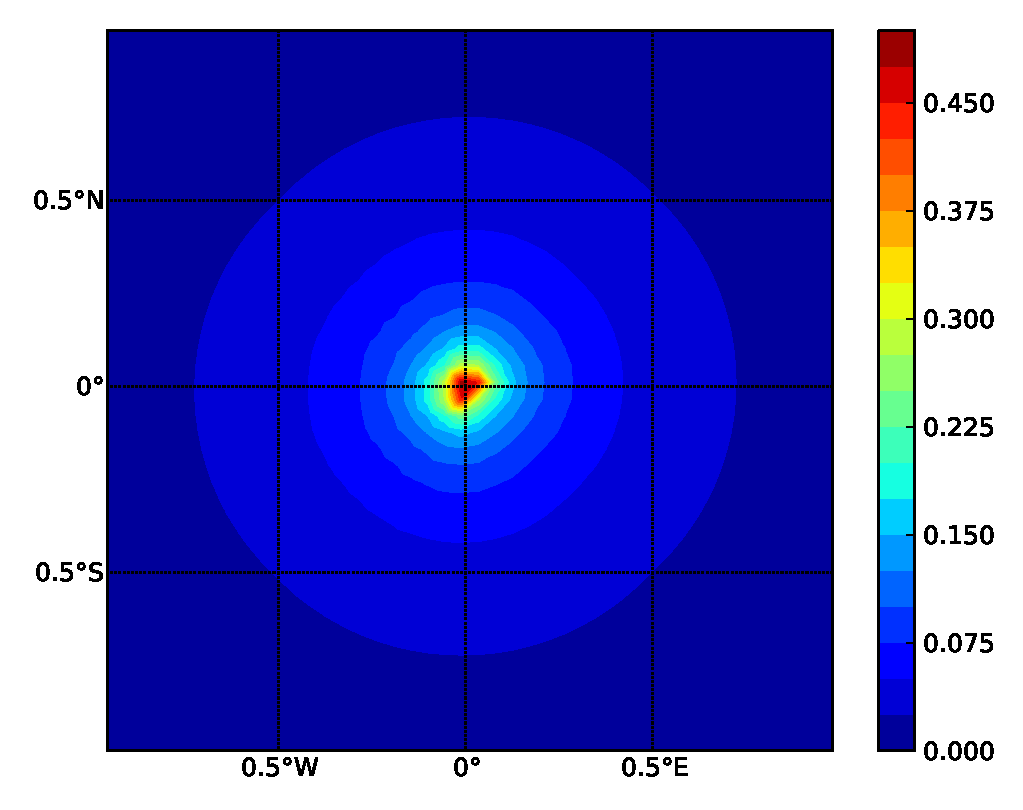
\includegraphics[width=7cm]{./figures/hazard/point.eps}} 
\subcaptionbox{}
{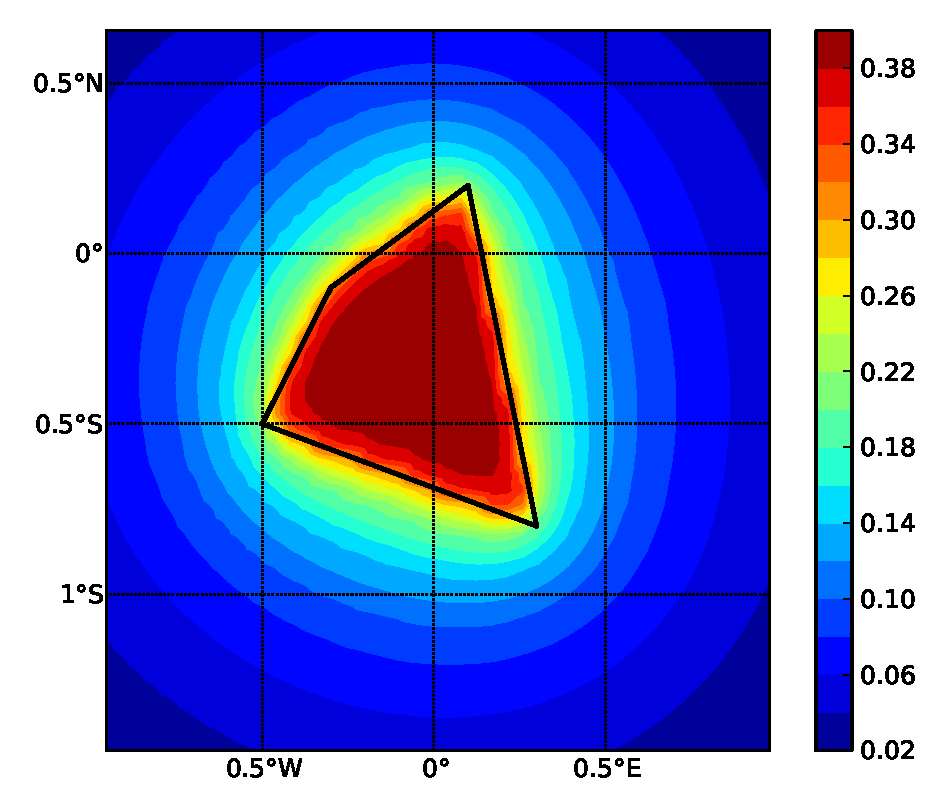
\includegraphics[width=7cm]{./figures/hazard/area.eps}} 
\subcaptionbox{}
{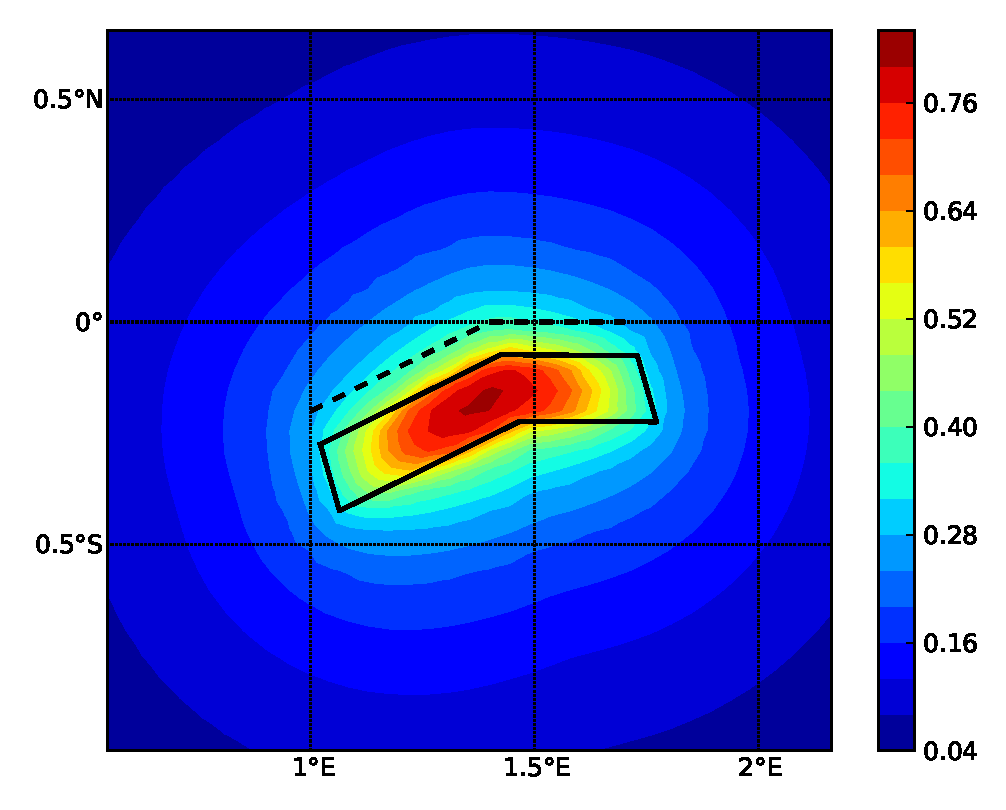
\includegraphics[width=7cm]{./figures/hazard/simple_fault.eps}} 
\subcaptionbox{}
{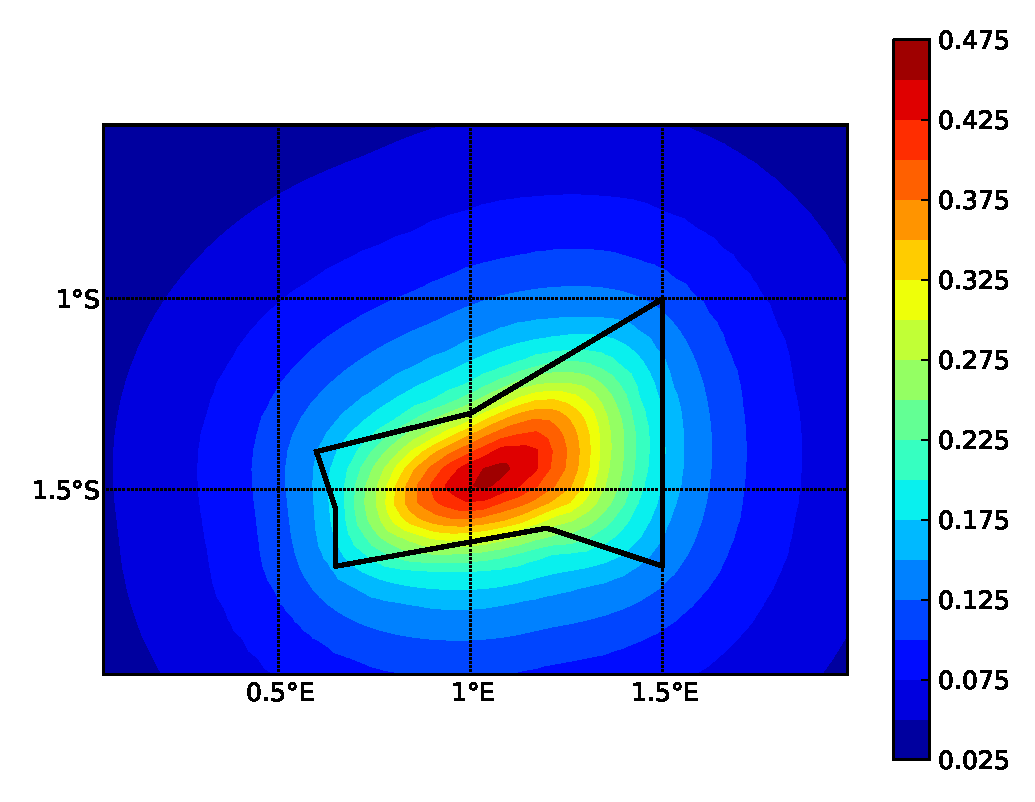
\includegraphics[width=7cm]{./figures/hazard/complex_fault.eps}} 
\caption{Hazard maps (for PGA, 10\% in 50 years) as obtained from the 
    different \gls{acr:oqe} source typologies. (a) Point Source. (b) Area 
    source.  The solid black line represents the area boundary. (c) Simple 
    Fault Source. 
    The dashed line represents the fault trace, while the solid line the fault
    surface projection. (d) Complex Fault Source. The solid line represent the 
    fault surface projection (d)}
\label{fig:hazard_maps1}
\end{figure}

\begin{figure} 
\centering 
\subcaptionbox{}
{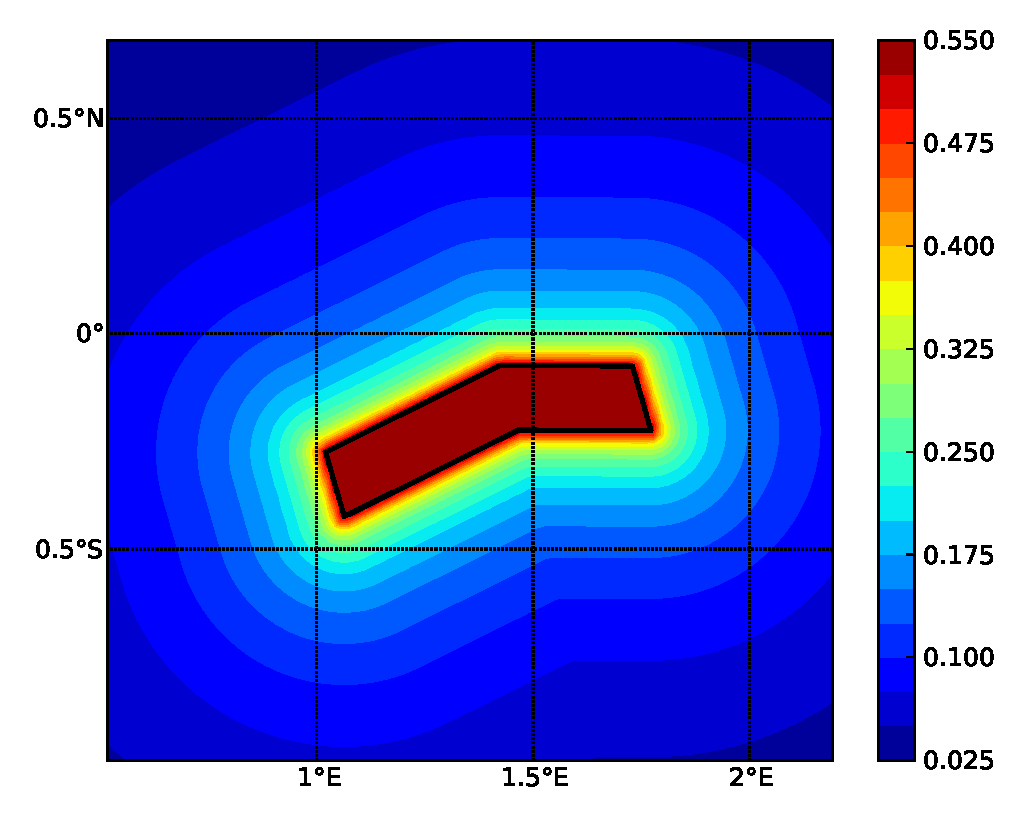
\includegraphics[width=7cm]{./figures/hazard/char_fault2.eps}} 
\subcaptionbox{}
{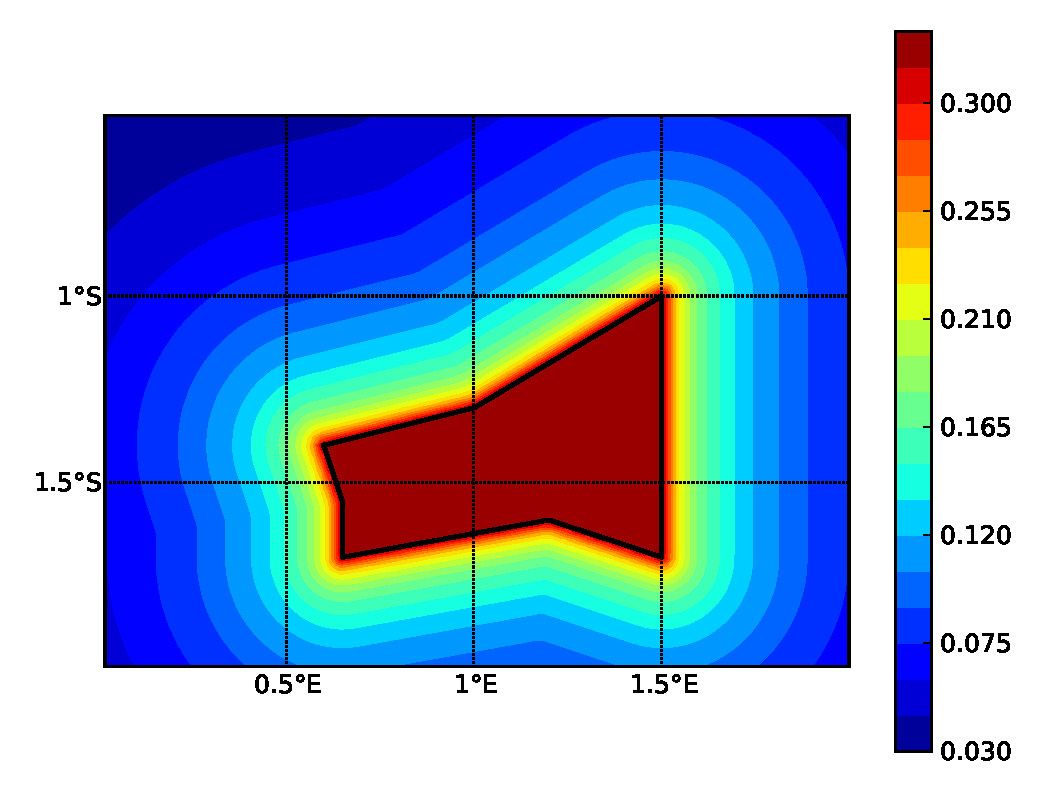
\includegraphics[width=7cm]{./figures/hazard/char_fault3.eps}} 
\subcaptionbox{}
{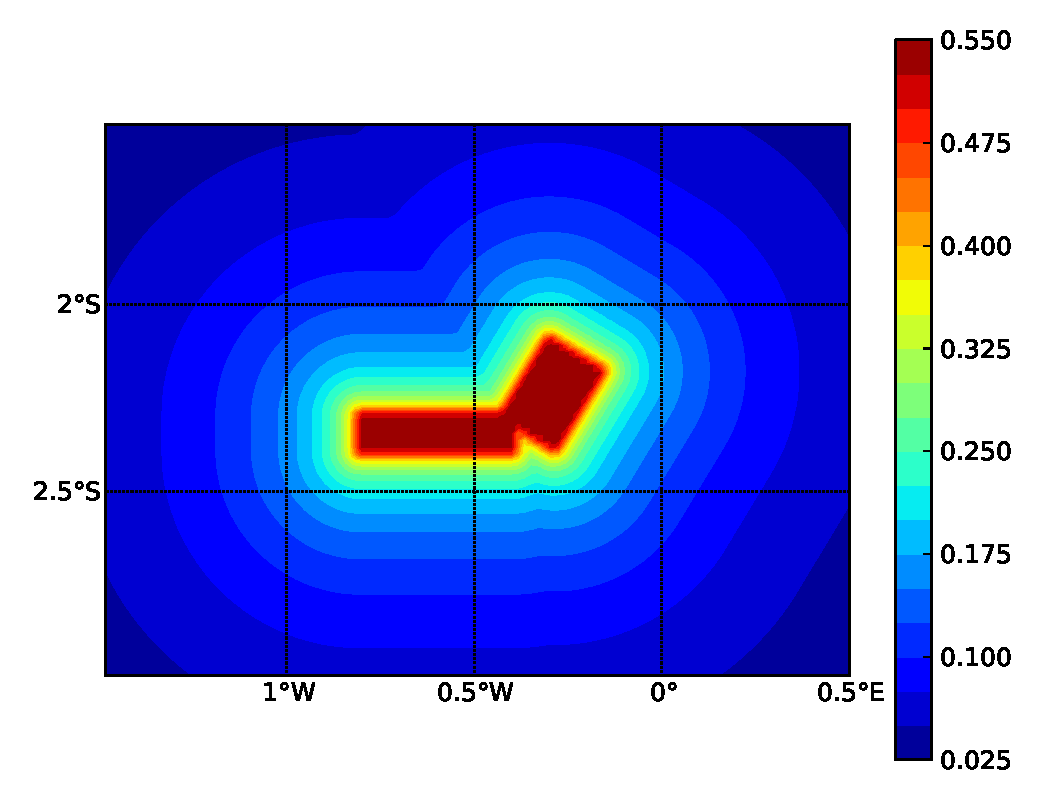
\includegraphics[width=7cm]{./figures/hazard/char_fault1.eps}} 
\caption{Hazard maps (for PGA, 10\% in 50 years) as obtained from 
    characteristic fault sources with simple fault
    geometry (e), complex fault geometry (f), and collection of 
    planar surfaces (g)}
\label{fig:hazard_maps2}
\end{figure}

\clearpage
\subsubsection{Classical PSHA with non trivial logic trees}
Three demos are provided to illustrate how the logic tree formalism can 
be used to express epistemic uncertainties in seismic hazard analysis.\\

LogicTreeCase1ClassicalPSHA shows an example of logic tree defining two 
alternative source models, with sources belonging to two different
tectonic region types, and with two alternative GMPEs for each tectonic 
region type.
The source model logic tree is therefore defined in the following way:
\begin{Verbatim}[frame=single, commandchars=\\\{\}, fontsize=\normalsize]
<?xml version="1.0" encoding="UTF-8"?>
<nrml xmlns:gml="http://www.opengis.net/gml"
      xmlns="http://openquake.org/xmlns/nrml/0.4">
    <logicTree logicTreeID="lt1">

        <logicTreeBranchingLevel branchingLevelID="bl1">

            <logicTreeBranchSet uncertaintyType="sourceModel"
                                branchSetID="bs1">
                <logicTreeBranch branchID="b1">
                    <uncertaintyModel>
                      source_model_1.xml
                    </uncertaintyModel>
                    <uncertaintyWeight>0.5</uncertaintyWeight>
                </logicTreeBranch>
                <logicTreeBranch branchID="b2">
                    <uncertaintyModel>
                       source_model_2.xml
                    </uncertaintyModel>
                    <uncertaintyWeight>0.5</uncertaintyWeight>
                </logicTreeBranch>
            </logicTreeBranchSet>

        </logicTreeBranchingLevel>

    </logicTree>
</nrml>
\end{Verbatim}
The two source models are defined in two separate files 
\texttt{source\_\-model\_\-1.xml} and \texttt{source\_\-model\_\-2.xml} each
one associated to a corresponding weight (0.5 for both).\\
The GSIM logic tree file contains the following structure:
\begin{Verbatim}[frame=single, commandchars=\\\{\}, fontsize=\normalsize]
<?xml version="1.0" encoding="UTF-8"?>

<nrml xmlns:gml="http://www.opengis.net/gml"
      xmlns="http://openquake.org/xmlns/nrml/0.4">
    <logicTree logicTreeID='lt1'>

        <logicTreeBranchingLevel branchingLevelID="bl1">
            <logicTreeBranchSet uncertaintyType="gmpeModel"
               applyToTectonicRegionType="Active Shallow Crust"
               branchSetID="bs1">
                <logicTreeBranch branchID="b11">
                   <uncertaintyModel>
                      BooreAtkinson2008
                   </uncertaintyModel>
                   <uncertaintyWeight>0.5</uncertaintyWeight>
                </logicTreeBranch>
                <logicTreeBranch branchID="b12">
                   <uncertaintyModel>
                      ChiouYoungs2008
                   </uncertaintyModel>
                   <uncertaintyWeight>0.5</uncertaintyWeight>
                </logicTreeBranch>
            </logicTreeBranchSet>
        </logicTreeBranchingLevel>

        <logicTreeBranchingLevel branchingLevelID="bl2">
            <logicTreeBranchSet uncertaintyType="gmpeModel"
              applyToTectonicRegionType="Stable Continental Crust"
              branchSetID="bs2">
              <logicTreeBranch branchID="b21">
                <uncertaintyModel>
                   ToroEtAl2002</uncertaintyModel>
                <uncertaintyWeight>0.5</uncertaintyWeight>
                </logicTreeBranch>
                <logicTreeBranch branchID="b22">
                  <uncertaintyModel>
                     Campbell2003</uncertaintyModel>
                  <uncertaintyWeight>0.5</uncertaintyWeight>
                </logicTreeBranch>
            </logicTreeBranchSet>
        </logicTreeBranchingLevel>

    </logicTree>
</nrml>
\end{Verbatim}
The source model contains sources belonging to Active Shallow Crust and 
Stable Continental Crust, therefore the
GSIM logic tree defines two branching levels, one for each considered 
tectonic region type. Moreover for each tectonic
region a branch set with two GMPEs is defined: Boore and Atkinson 
2008 and Chiou and Youngs 2008 for Active
Shallow Crust and Toro et al. 2003 and Campbell 2003 for Stable Continental 
Crust. By processing the above logic tree
files using the logic tree path enumeration mode (enabled by setting in the 
configuration file \texttt{number\_\-of\_\-logic\_\-tree\_\-samples = 0})
hazard results are computed for 8 logic tree paths (2 source models x 2 GMPEs
for Active x 2 GMPEs for Stable).\\

LogicTreeCase2ClassicalPSHA defines a single source model consisting of 
only two sources (area and simple fault) belonging to different
tectonic region types (Active Shallow Crust and Stable Continental Region) 
and both characterized by a truncated Gutenberg-Richter distribution.
The logic tree defines uncertainties for G-R a and b values (three possible
pairs for each source), maximum magnitude (three values for each source) 
and uncertainties on the GMPEs for each tectonic region type (two GMPE per 
region type).\\
To accommodate such a structure the GSIM logic tree is defined in the
following way:
\begin{Verbatim}[frame=single, commandchars=\\\{\}, fontsize=\normalsize]
<?xml version="1.0" encoding="UTF-8"?>
<nrml xmlns:gml="http://www.opengis.net/gml"
      xmlns="http://openquake.org/xmlns/nrml/0.4">
    <logicTree logicTreeID="lt1">

        <logicTreeBranchingLevel branchingLevelID="bl1">
            <logicTreeBranchSet uncertaintyType="sourceModel"
                                branchSetID="bs1">
                <logicTreeBranch branchID="b11">
                    <uncertaintyModel>
                     source_model.xml
                    </uncertaintyModel>
                    <uncertaintyWeight>1.0</uncertaintyWeight>
                </logicTreeBranch>
            </logicTreeBranchSet>
        </logicTreeBranchingLevel>

        <logicTreeBranchingLevel branchingLevelID="bl2">
            <logicTreeBranchSet uncertaintyType="abGRAbsolute"
                                applyToSources="1"
                                branchSetID="bs21">
                <logicTreeBranch branchID="b21">
                    <uncertaintyModel>4.6 1.1</uncertaintyModel>
                    <uncertaintyWeight>0.333</uncertaintyWeight>
                </logicTreeBranch>
                <logicTreeBranch branchID="b22">
                    <uncertaintyModel>4.5 1.0</uncertaintyModel>
                    <uncertaintyWeight>0.333</uncertaintyWeight>
                </logicTreeBranch>
                <logicTreeBranch branchID="b23">
                    <uncertaintyModel>4.4 0.9</uncertaintyModel>
                    <uncertaintyWeight>0.334</uncertaintyWeight>
                </logicTreeBranch>
            </logicTreeBranchSet>
        </logicTreeBranchingLevel>

        <logicTreeBranchingLevel branchingLevelID="bl3">
            <logicTreeBranchSet uncertaintyType="abGRAbsolute"
                                applyToSources="2"
                                branchSetID="bs31">
                <logicTreeBranch branchID="b31">
                    <uncertaintyModel>3.3 1.0</uncertaintyModel>
                    <uncertaintyWeight>0.333</uncertaintyWeight>
                </logicTreeBranch>
                <logicTreeBranch branchID="b32">
                    <uncertaintyModel>3.2 0.9</uncertaintyModel>
                    <uncertaintyWeight>0.333</uncertaintyWeight>
                </logicTreeBranch>
                <logicTreeBranch branchID="b33">
                    <uncertaintyModel>3.1 0.8</uncertaintyModel>
                    <uncertaintyWeight>0.334</uncertaintyWeight>
                </logicTreeBranch>
            </logicTreeBranchSet>
        </logicTreeBranchingLevel>

        <logicTreeBranchingLevel branchingLevelID="bl4">
            <logicTreeBranchSet uncertaintyType="maxMagGRAbsolute"
                                applyToSources="1"
                                branchSetID="bs41">
                <logicTreeBranch branchID="b41">
                    <uncertaintyModel>7.0</uncertaintyModel>
                    <uncertaintyWeight>0.333</uncertaintyWeight>
                </logicTreeBranch>
                <logicTreeBranch branchID="b42">
                    <uncertaintyModel>7.3</uncertaintyModel>
                    <uncertaintyWeight>0.333</uncertaintyWeight>
                </logicTreeBranch>
                <logicTreeBranch branchID="b43">
                    <uncertaintyModel>7.6</uncertaintyModel>
                    <uncertaintyWeight>0.334</uncertaintyWeight>
                </logicTreeBranch>
            </logicTreeBranchSet>
        </logicTreeBranchingLevel>

        <logicTreeBranchingLevel branchingLevelID="bl5">
            <logicTreeBranchSet uncertaintyType="maxMagGRAbsolute"
                                applyToSources="2"
                                branchSetID="bs51">
                <logicTreeBranch branchID="b51">
                    <uncertaintyModel>7.5</uncertaintyModel>
                    <uncertaintyWeight>0.333</uncertaintyWeight>
                </logicTreeBranch>
                <logicTreeBranch branchID="b52">
                    <uncertaintyModel>7.8</uncertaintyModel>
                    <uncertaintyWeight>0.333</uncertaintyWeight>
                </logicTreeBranch>
                <logicTreeBranch branchID="b53">
                    <uncertaintyModel>8.0</uncertaintyModel>
                    <uncertaintyWeight>0.334</uncertaintyWeight>
                </logicTreeBranch>
            </logicTreeBranchSet>
        </logicTreeBranchingLevel>

    </logicTree>
</nrml>
\end{Verbatim}
The first branching level defines the source model. For each source, 
two branching levels are created, one defining
uncertainties on G-R a and b values (defined by setting 
\texttt{uncertaintyType="abGRAbsolute"}) and G-R maximum
magnitude (\texttt{uncertaintyType="maxMagGRAbsolute"}). 
%
It is important to notice that each branch set is applied
to a specific source by defining the attribute \texttt{apply\-To\-Sources}, 
followed by the source ID. The GSIM logic tree file is
the same as used for LogicTreeCase1ClassicalPSHA. By setting in the 
configuration file \texttt{number\_\-of\_\-logic\_\-tree\_\-samples = 0},
hazard results are obtained for 324 paths (1 source model x 3 (a, b) 
pairs for source 1 x  3 (a, b) pairs for source 2 x 3 max magnitude values
for source 1 x 3 max magnitude values for source 2 x 2 GMPEs for Active 
Shallow Crust X 2 GMPEs for Stable Continental Crust), see
figure \ref{fig:hazard_curves}.\\

\begin{figure} 
\centering 
\subcaptionbox{}
{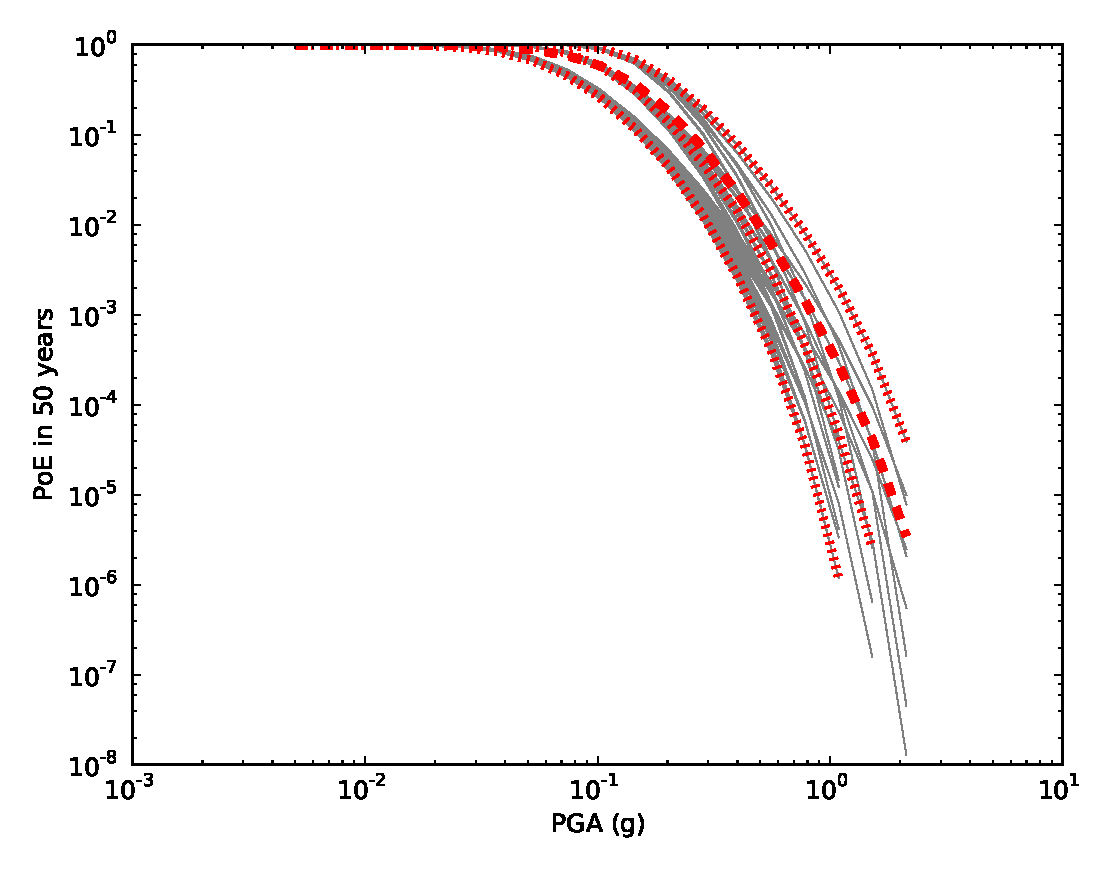
\includegraphics[width=9cm]{./figures/hazard/hazard-curves-ltcase2.eps}} 
\caption{Hazard curves as obtained from the LogicTreeCase2 demo. Solid gray 
    lines represent individual hazard curves from the different
    logic tree path (a total of 324 curves). The red dashed line represents the
    mean hazard curve, while the red dotted lines depict the quantile levels
    (0.15, 0.5, 0.95).}
\label{fig:hazard_curves}
\end{figure}

LogicTreeCase3ClassicalPSHA illustrates an example of logic tree defining 
relative uncertainties on G-R maximum magnitude and b value.
A single source model is considered containing two sources belonging to 
different tectonic region types and both characterized by a G-R 
magnitude frequency distribution. The source model logic tree is as follows:
\begin{Verbatim}[frame=single, commandchars=\\\{\}, fontsize=\normalsize]
<?xml version="1.0" encoding="UTF-8"?>
<nrml xmlns:gml="http://www.opengis.net/gml"
      xmlns="http://openquake.org/xmlns/nrml/0.4">
    <logicTree logicTreeID="lt1">

        <logicTreeBranchingLevel branchingLevelID="bl1">
            <logicTreeBranchSet uncertaintyType="sourceModel"
                                branchSetID="bs1">
                <logicTreeBranch branchID="b11">
                    <uncertaintyModel>
                     source_model.xml
                    </uncertaintyModel>
                    <uncertaintyWeight>1.0</uncertaintyWeight>
                </logicTreeBranch>
            </logicTreeBranchSet>
        </logicTreeBranchingLevel>

        <logicTreeBranchingLevel branchingLevelID="bl2">
            <logicTreeBranchSet uncertaintyType="bGRRelative"
                                branchSetID="bs21">
                <logicTreeBranch branchID="b21">
                    <uncertaintyModel>+0.1</uncertaintyModel>
                    <uncertaintyWeight>0.333</uncertaintyWeight>
                </logicTreeBranch>
                <logicTreeBranch branchID="b22">
                    <uncertaintyModel>0.0</uncertaintyModel>
                    <uncertaintyWeight>0.333</uncertaintyWeight>
                </logicTreeBranch>
                <logicTreeBranch branchID="b23">
                    <uncertaintyModel>-0.1</uncertaintyModel>
                    <uncertaintyWeight>0.334</uncertaintyWeight>
                </logicTreeBranch>
            </logicTreeBranchSet>
        </logicTreeBranchingLevel>

        <logicTreeBranchingLevel branchingLevelID="bl3">
            <logicTreeBranchSet uncertaintyType="maxMagGRRelative"
                                branchSetID="bs31">
                <logicTreeBranch branchID="b31">
                    <uncertaintyModel>0.0</uncertaintyModel>
                    <uncertaintyWeight>0.333</uncertaintyWeight>
                </logicTreeBranch>
                <logicTreeBranch branchID="b32">
                    <uncertaintyModel>+0.5</uncertaintyModel>
                    <uncertaintyWeight>0.333</uncertaintyWeight>
                </logicTreeBranch>
                <logicTreeBranch branchID="b33">
                    <uncertaintyModel>+1.0</uncertaintyModel>
                    <uncertaintyWeight>0.334</uncertaintyWeight>
                </logicTreeBranch>
            </logicTreeBranchSet>
        </logicTreeBranchingLevel>

    </logicTree>
</nrml>
\end{Verbatim}
After the first branching level defining the source model, two 
additional branching levels are defined, one defining
relative uncertainties on b value (\texttt{bGR\-Rel\-a\-tive} applied 
consistently to all sources in the source model)
and the second uncertainties on maximum magnitude (\texttt{maxMagGRRelative}). 
Similarly to the other cases, two GMPEs are considered for each tectonic 
region type and therefore the total number of logic tree path is 36
(1 source model x 3 b value increments x 3 maximum magnitude increments 
x 2 GMPE for Active x 2 GMPEs for Stable)

\subsubsection{Event Based PSHA}
A demo showing an example of Event Based calculation is provided with the 
following configuration file:
\begin{Verbatim}[frame=single, commandchars=\\\{\}, fontsize=\normalsize]
[general]

description = Event Based PSHA using Area Source
calculation_mode = event_based
random_seed = 23

[geometry]

sites = 0.5 -0.5

[logic_tree]

number_of_logic_tree_samples = 0

[erf]

rupture_mesh_spacing = 2
width_of_mfd_bin = 0.1
area_source_discretization = 5.0

[site_params]

reference_vs30_type = measured
reference_vs30_value = 600.0
reference_depth_to_2pt5km_per_sec = 5.0
reference_depth_to_1pt0km_per_sec = 100.0

[calculation]

source_model_logic_tree_file = source_model_logic_tree.xml
gsim_logic_tree_file = gmpe_logic_tree.xml
investigation_time = 50.0
intensity_measure_types = PGA
intensity_measure_types_and_levels = {"PGA": [...]}
truncation_level = 3
maximum_distance = 200.0

[event_based_params]

ses_per_logic_tree_path = 100
ground_motion_correlation_model =
ground_motion_correlation_params =

[output]

export_dir = ...
ground_motion_fields = true
hazard_curves_from_gmfs = true
mean_hazard_curves = false
quantile_hazard_curves =
hazard_maps = true
poes = 0.1
\end{Verbatim}
The source model consist of one source (area). 100 stochastic event sets 
are generated (\texttt{ses\_\-per\_\-logic\_\-tree\_\-path = 100}) (an 
example can be seen in figure \ref{fig:ses}). Ground motion fields are 
computed (\texttt{ground\_\-motion\_\-fields = true}, figure \ref{fig:gmfs}) 
and also hazard curves from ground motion fields are
extracted (\texttt{hazard\_\-curves\_\-from\_\-gmfs = true}).
The corresponding hazard maps for 0.1 probability are also calculated
(\texttt{hazard\_\-maps = true})

\begin{figure} 
\centering 
\subcaptionbox{}
{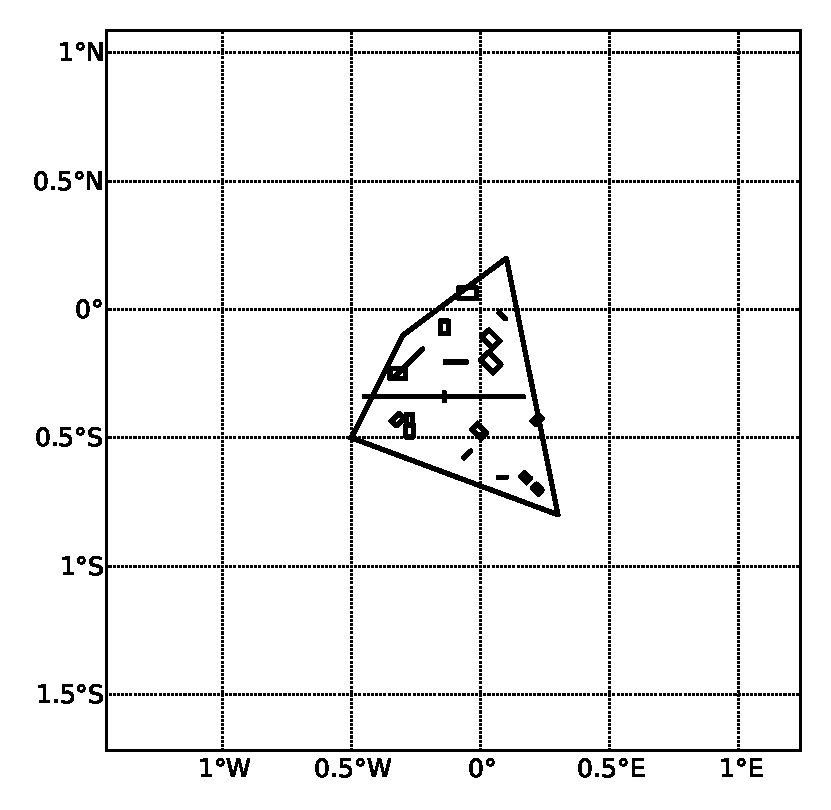
\includegraphics[width=9cm]{./figures/hazard/ses.eps}} 
\caption{A stochastic event set generated with the event based PSHA demo. 
    The area source defines a nodal plane distribution which distributes 
    events among vertical and dipping (50 degrees) faults with equal weights. 
    Vertical ruptures are then distributed equally in the range 0-180 degrees 
    while the dipping ones in the range 0-360, both with a step of 45 degrees.}
\label{fig:ses}
\end{figure}

\begin{figure} 
\centering 
\subcaptionbox{}
{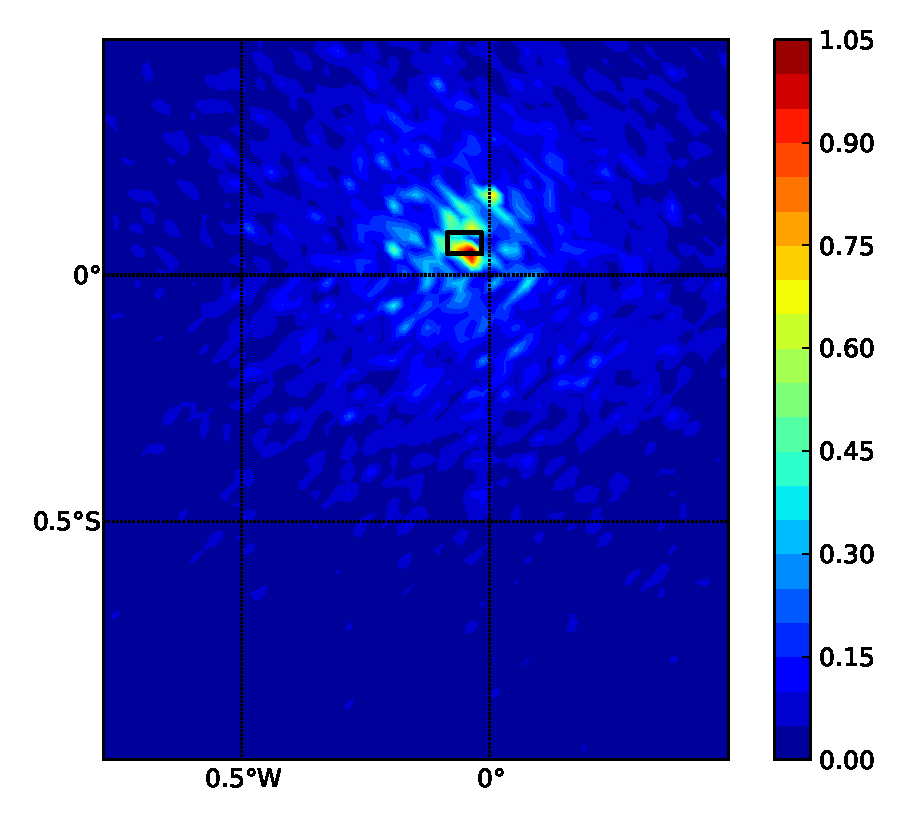
\includegraphics[width=6cm]{./figures/hazard/gmf-no-corr.eps}} 
\subcaptionbox{}
{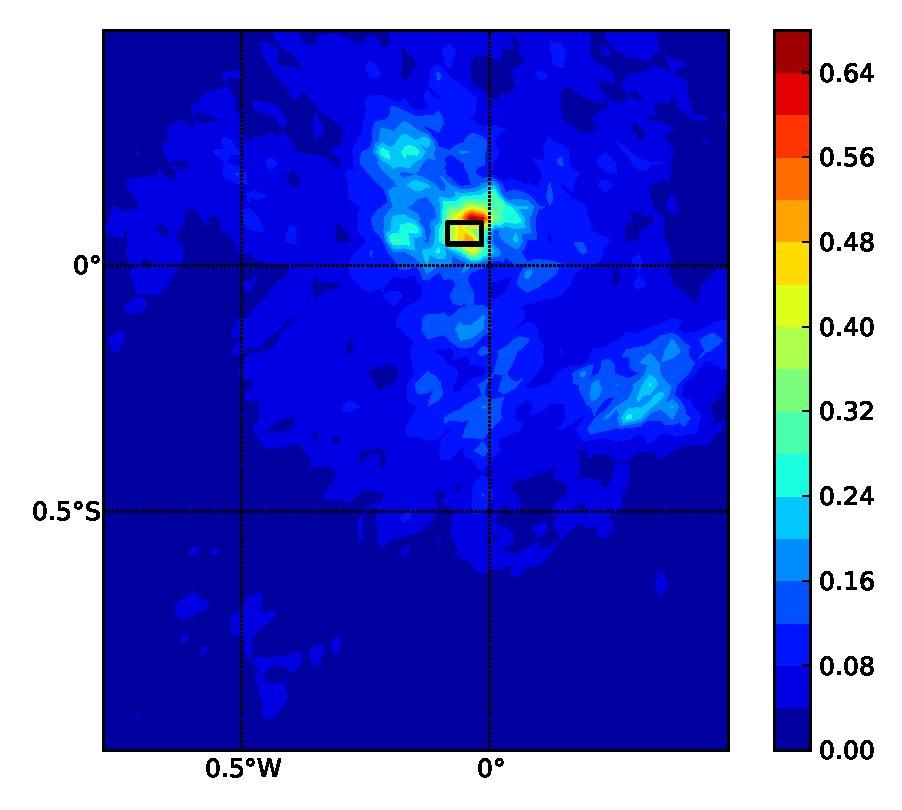
\includegraphics[width=6cm]{./figures/hazard/gmf-corr.eps}} 
\caption{Ground motion fields (PGA) with no spatial correlations (a) and with spatial correlation (b)}
\label{fig:gmfs}
\end{figure}

\subsubsection{Disaggregation}
An example of disaggregation calculation is given considering a source model 
consisting of two sources (area and simple fault) belonging to two different 
tectonic region types.

The calculation is defined with the following configuration file:
\begin{Verbatim}[frame=single, commandchars=\\\{\}, fontsize=\normalsize]
[general]

description = ...
calculation_mode = disaggregation
random_seed = 23

[geometry]

sites = 0.5 -0.5

[logic_tree]

number_of_logic_tree_samples = 0

[erf]

rupture_mesh_spacing = 2
width_of_mfd_bin = 0.1
area_source_discretization = 5.0

[site_params]

reference_vs30_type = measured
reference_vs30_value = 600.0
reference_depth_to_2pt5km_per_sec = 5.0
reference_depth_to_1pt0km_per_sec = 100.0

[calculation]

source_model_logic_tree_file = source_model_logic_tree.xml
gsim_logic_tree_file = gmpe_logic_tree.xml
investigation_time = 50.0
intensity_measure_types_and_levels = {"PGA": [...]}
truncation_level = 3
maximum_distance = 200.0

[disaggregation]

poes_disagg = 0.1
mag_bin_width = 1.0
distance_bin_width = 10.0
coordinate_bin_width = 0.2
num_epsilon_bins = 3

[output]

export_dir = ...
\end{Verbatim}
Disaggregation matrices are computed for a single site (located between the two sources) for a ground motion value corresponding to a probability value equal to 0.1
(\texttt{poes\_\-disagg = 0.1}). Magnitude values are classified in one magnitude unit bins (\texttt{mag\_\-bin\_\-width = 1.0}), distances in bins of 10 km
(\texttt{distance\_\-bin\_\-width = 10.0}), coordinates in bins of 0.2 degrees (\texttt{coordinate\_\-bin\_\-width = 0.2}). 3 epsilons bins are considered (\texttt{num\_\-epsilon\_\-bins = 3}).

\begin{comment}
The demo allows to compute 

\section{Demo 01 - Classical PSHA}

% -----------------------------------------------------------------------------
\section{Demo 02 - Classical PSHA: simple logic tree}
This demo contains simple logic tree structures accounting for epistemic
uncertainties in the seismic source and ground motion intensity models.

The seismic source model incorporates epistemic uncertainty about the 
value of the maximum magnitude of the magnitude-frequency distribution 
used.
%
The ground motion intensity model includes uncertainty about the ground
motion prediction equations to be used in the calculation of hazard.

Given that the overall structure of the logic tree is not particularly
complex and assuming that uncertainties are fully correlated we decide 
to compute all the possible realisations of the logic tree by fixing 
the \texttt{number\_\-of\_\-logic\_\-tree\_\-samples} parameter in the 
configuration file to zero.
\begin{Verbatim}[frame=single, commandchars=\\\{\}, fontsize=\normalsize]
[logic_tree]
number_of_logic_tree_samples = 0
\end{Verbatim}

Let's now run the OpenQuake:
\begin{Verbatim}[frame=single, fontsize=\normalsize]
user@ubuntu:~/demos/classical_psha_simple_lt$ openquake \ 
--rh job_1strike.ini 
\end{Verbatim}

This is the list of results that we get at the end of this calculation:
\begin{Verbatim}[frame=single, commandchars=\\\{\}, fontsize=\normalsize]
Calculation 8 results:
id | output_type | name
5 | hazard_curve | hc-rlz-10
6 | hazard_curve | hc-rlz-7
7 | hazard_curve | hc-rlz-8
8 | hazard_curve | hc-rlz-9
9 | hazard_curve | hc-rlz-11
10 | hazard_curve | hc-rlz-12
11 | hazard_map | hazard-map(0.1)-PGA-rlz-10
12 | hazard_map | hazard-map(0.1)-PGA-rlz-7
13 | hazard_map | hazard-map(0.1)-PGA-rlz-8
14 | hazard_map | hazard-map(0.1)-PGA-rlz-9
15 | hazard_map | hazard-map(0.1)-PGA-rlz-11
16 | hazard_map | hazard-map(0.1)-PGA-rlz-12
\end{Verbatim}
OpenQuake produced six hazard curves and six hazard maps i.e. one
result for each leaf of the logic tree. 
\end{comment}

% ==============================================================================
% ------------------------------------------------------------------------- Part
\part{Risk}
% ------------------------------------------------------------------------------
%\chapter{Introduction}
%	This book aims to provide an explanation of the scientific basis 
and the methodologies adopted in the implementation of the OpenQuake engine, an open source code for seismic hazard and physical risk calculation. 
%
The book follows the traditional openness and transparency features of the 
\gls{acr:gem} as clearly indicated in the development principles of 
the OpenQuake engine. 

%
The \gls{acr:gem} initiative is a global collaborative effort with the aim to provide organisations and people with tools and resources for transparent assessment of earthquake risk anywhere in the world.
%
The OpenQuake engine is a fully integrated, flexible and scalable hazard and physical risk 
calculation engine whose development is at the core of \gls{acr:gem}'s
overall objectives.
% ------------------------------------------------------------------------------
\section{Basics of the Engine}
The implementation of the OpenQuake software officially started in Summer 2010 
following the experience gained in \gls{acr:gem}'s kick-off project GEM1 
\citep{gemfoundation2010}, during which an extensive appraisal of existing hazard 
and physical risk codes was performed \citep{danciu2010,crowley2010}
and prototype hazard and risk software were selected, designed and
implemented \citep{pagani2010,crowley2010a}.

The current version of the OpenQuake engine is Python code developed 
following the most common requirements of Open Source 
software development, such as a public repository, IRC channel and open mailing lists. 
The source code, released under an open source software license,
is freely and openly accessible on a web based repository 
(see \href{http://github.com/gem}{github.com/gem}) while the 
development process is managed so that the community can participate 
to the day by day development as well as in the mid- and long-term 
design process. 
%
The software development also leverages on a number of open source projects 
such as \href {http://celeryproject.org}{Celeryd} and \href{http://www.rabbitmq.com}{RabbitMQ}, just to mention a few.

The hazard component of the engine largely relies on classes belonging to the OpenQuake Hazard library (see \href{https://github.com/gem/oq-hazardlib}{oq-hazardlib}) a comprehensive library for performing state-or-the-art PSHA. This library has been designed and implemented following the successful collaboration and important lessons learnt working with the \href{http://www.opensha.org}{OpenSHA} software and the developing teams at \gls{acr:usgs} and 
\gls{acr:scec} in GEM1. 
%
The risk component of the engine was designed in GEM1, prototyped in Java and eventually
coded in Python by the team operating at the \gls{acr:gem} 
Model Facility. This scientific code was originally integrated with the engine, but in late 2012 it was extracted to form the OpenQuake Risk Library (see \href{https://github.com/gem/oq-risklib}{oq-risklib}).

%A schema that illustrates the structure of the engine is 
%represented in Figure \ref{fig:openquake_schema}; the schema contains:
%purple boxes representing the main modules of the hazard component, 
%green boxes showing the modules of the risk component, white boxes
%with main outputs computed by the distinct modules and orange rectangles
%displaying the main input information that should be entered into the calculation engine. 
%
% ------------------------------------------------------------------------------
%\subsection{Brief description of the OpenQuake IT architecture}
%% ------------------------------------------------------------------------------
Openquake is the core of the OpenGEM system. 
%
As it appears in Figure \ref{fig:oq_it}, OpenQuake is powered by a 
number of open source software projects, of which OpenSHA-lite and 
RiskLib are currently the most essential ones. 
OpenSHA-lite is a ‘light’ version of the comprehensive software for 
probabilistic seismic hazard assessment OpenSHA and whose code serves
as a basis for the hazard component of the OpenQuake engine. RiskLib 
is a global collaboration project that is aimed at common development 
of a code ‘library’ for the risk all types of natural hazards, including
an API, on wh ich ‘apps’ can be built, such as tools that support risk
mitigation/reduction. The World Bank’s GFDRR, OpenGeo, AIFDR and GEM 
jointly work on RiskLib and its code repository, currently part of 
the OpenQuake project, will be broken out soon.
%
% . . . . . . . . . . . . . . . . . . . . . . . . . . . . . . . . . . . > Figure
\begin{figure}
\includegraphics[width=\textwidth,angle=0]{./Figures/Part_Introduction/oq_system_architecture.eps}
\caption{Openquake system architecture.}
\label{fig:oq_it}
\end{figure}
% . . . . . . . . . . . . . . . . . . . . . . . . . . . . . . . . . . . < Figure
%
Implementation of a standard format for data exchange for natural hazard
and risk,  is closely related to what is described above. The NRML 
(Natural hazards’ Risk Markup Language) format has been developed, which
is capable of encompassing a wide variety of risk and hazard data formats.
More information can be found in the detailed background documentation 
for OpenQuake.

The data services that are mentioned above are globally accessible 
read/write collaborations of core data sets that are exposed with a 
REST API. Some of the core modules of GEM will be available through 
the services and are currently being developed by GEM’s Model Facility 
development team, in collaboration with a number of IT partners and the 
scientists coordinating the modules. Examples are the development of a 
global exposure database, development of a global portal for active 
faults, global vulnerability functions and an earthquake consequences
database.






%
% ------------------------------------------------------------------------------
\section{Structure of the Book}
The OpenQuake Engine Book is organized into two volumes, one which describes the science behind the hazard component of the engine
and another which illustrates the theory of the physical risk calculators incorporated into the software. Readers that are interested in learning how to run calculations using the OpenQuake engine are referred to the OpenQuake Engine User Manual.

\hfill \\
%\emph{Part II: Hazard}
The GEM Hazard Team is currently updating the volume on hazard. In the meantime, interested readers are referred to the OpenQuake Engine User Manual, or they can contact the coordinator, Dr Marco Pagani, for further information. 
%\begin{itemize}
%\item Chapter \ref{chap:inthaz} offers an introduction to the hazard 
%topics discussed in the following chapters. In particular, in this 
%Chapter we discuss the main OpenQuake concepts and we illustrate the 
%calculation workflows currently available in the hazard component of 
%OpenQuake.
%\item Chapter \ref{chap:hazinp} focuses on the structure and the 
%characteristics of the information necessary to define a 
%comprehensive PSHA input model. This Chapter also includes
%descriptions of the main seismic source typologies and of the logic 
%tree structure.
%\item We dedicate Chapter \ref{chap:erf} to the explanation of the
%methodology adopted for the processing of the logic tree structures
%supported by OpenQuake and for the creation of the 
%\gls{earthquakeruptureforecast}
%\item The last Chapter of the hazard part (chapter \ref{chap:hazcalc}) 
%illustrates the main calculators available: the classical-PSHA calculator,
%the event-based calculator and the disaggregation calculator. 
%\end{itemize}
\hfill \\
\hfill \\
%\emph{Part III: Risk}
This volume on risk is organised as follows:
\begin{itemize}
\item Chapter \ref{chap:intrisk} introduces the main physical risk concepts and workflows. 
\item Chapter \ref{chap:riskinput} contains an explanation of the exposure, physical vulnerability and fragility concepts, which are input to the calculations.
\item Chapter \ref{chap:scenario_risk} describes the scenario risk 
methodology, for estimating loss distributions for single events.
\item Chapter \ref{chap:scenario_damage} describes the scenario damage 
methodology, for estimating damage ditributions for single events.
\item Chapter \ref{chap:risk_prob_event_based} provides an overview of the probabilistic event-based risk calculation methodology, which produces loss exceedance curves for portfolios of buildings.
\item Chapter \ref{chap:risk_psha_based} illustrates single-site risk calculations based on the hazard curves from classical PSHA.
\item Chapter \ref{chap:bcr} outlines the benefit/cost ratio calculations based on loss curves for structures with and without retrofitting.
\end{itemize}
%
%In the closing part, the Book contains a glossary that aims to define a 
%clear and unique terminology.
%
% . . . . . . . . . . . . . . . . . . . . . . . . . . . . . . . . . . . > Figure
%\begin{landscape}
%\begin{figure}
%\includegraphics[width=20cm,angle=0]{./Figures/Part_Introduction/engine9_20110130.eps}
%\caption{OpenQuake Engine schema. Purple boxes are the calculators included in the  
%the hazard part of OQ; green boxes are the physical risk calculators.}
%\label{fig:openquake_schema}
%\end{figure}
%\end{landscape}
% . . . . . . . . . . . . . . . . . . . . . . . . . . . . . . . . . . . < Figure
% ------------------------------------------------------------------------------
%\chapter{OpenQuake risk input description}
%	\label{chap:riskinp}
%	\input{./oqum/part_risk_calc/riskInputDescription.tex}
% ------------------------------------------------------------------------------
%\chapter{OpenQuake risk calculation examples}
%	\label{chap:riskexamples}
%	\input{./oqum/part_Risk_Calc/riskCalcExamples.tex}
	
%\chapter{OpenQuake risk configuration parameters}	
%	\label{chap:riskconfigpar}
%	\input{./oqum/part_risk_calc/riskConfigParam.tex}	
%
%\chapter{OpenQuake risk output description}	
%	\label{chap:riskout}
%	\input{./oqum/part_risk_calc/riskOutputDescription.tex}	
	
% ==============================================================================
% ------------------------------------------------------------------------- Part
%\part{Modeller's Toolkit}
% ------------------------------------------------------------------------------
%\chapter{Introduction}
%	This book aims to provide an explanation of the scientific basis 
and the methodologies adopted in the implementation of the OpenQuake engine, an open source code for seismic hazard and physical risk calculation. 
%
The book follows the traditional openness and transparency features of the 
\gls{acr:gem} as clearly indicated in the development principles of 
the OpenQuake engine. 

%
The \gls{acr:gem} initiative is a global collaborative effort with the aim to provide organisations and people with tools and resources for transparent assessment of earthquake risk anywhere in the world.
%
The OpenQuake engine is a fully integrated, flexible and scalable hazard and physical risk 
calculation engine whose development is at the core of \gls{acr:gem}'s
overall objectives.
% ------------------------------------------------------------------------------
\section{Basics of the Engine}
The implementation of the OpenQuake software officially started in Summer 2010 
following the experience gained in \gls{acr:gem}'s kick-off project GEM1 
\citep{gemfoundation2010}, during which an extensive appraisal of existing hazard 
and physical risk codes was performed \citep{danciu2010,crowley2010}
and prototype hazard and risk software were selected, designed and
implemented \citep{pagani2010,crowley2010a}.

The current version of the OpenQuake engine is Python code developed 
following the most common requirements of Open Source 
software development, such as a public repository, IRC channel and open mailing lists. 
The source code, released under an open source software license,
is freely and openly accessible on a web based repository 
(see \href{http://github.com/gem}{github.com/gem}) while the 
development process is managed so that the community can participate 
to the day by day development as well as in the mid- and long-term 
design process. 
%
The software development also leverages on a number of open source projects 
such as \href {http://celeryproject.org}{Celeryd} and \href{http://www.rabbitmq.com}{RabbitMQ}, just to mention a few.

The hazard component of the engine largely relies on classes belonging to the OpenQuake Hazard library (see \href{https://github.com/gem/oq-hazardlib}{oq-hazardlib}) a comprehensive library for performing state-or-the-art PSHA. This library has been designed and implemented following the successful collaboration and important lessons learnt working with the \href{http://www.opensha.org}{OpenSHA} software and the developing teams at \gls{acr:usgs} and 
\gls{acr:scec} in GEM1. 
%
The risk component of the engine was designed in GEM1, prototyped in Java and eventually
coded in Python by the team operating at the \gls{acr:gem} 
Model Facility. This scientific code was originally integrated with the engine, but in late 2012 it was extracted to form the OpenQuake Risk Library (see \href{https://github.com/gem/oq-risklib}{oq-risklib}).

%A schema that illustrates the structure of the engine is 
%represented in Figure \ref{fig:openquake_schema}; the schema contains:
%purple boxes representing the main modules of the hazard component, 
%green boxes showing the modules of the risk component, white boxes
%with main outputs computed by the distinct modules and orange rectangles
%displaying the main input information that should be entered into the calculation engine. 
%
% ------------------------------------------------------------------------------
%\subsection{Brief description of the OpenQuake IT architecture}
%% ------------------------------------------------------------------------------
Openquake is the core of the OpenGEM system. 
%
As it appears in Figure \ref{fig:oq_it}, OpenQuake is powered by a 
number of open source software projects, of which OpenSHA-lite and 
RiskLib are currently the most essential ones. 
OpenSHA-lite is a ‘light’ version of the comprehensive software for 
probabilistic seismic hazard assessment OpenSHA and whose code serves
as a basis for the hazard component of the OpenQuake engine. RiskLib 
is a global collaboration project that is aimed at common development 
of a code ‘library’ for the risk all types of natural hazards, including
an API, on wh ich ‘apps’ can be built, such as tools that support risk
mitigation/reduction. The World Bank’s GFDRR, OpenGeo, AIFDR and GEM 
jointly work on RiskLib and its code repository, currently part of 
the OpenQuake project, will be broken out soon.
%
% . . . . . . . . . . . . . . . . . . . . . . . . . . . . . . . . . . . > Figure
\begin{figure}
\includegraphics[width=\textwidth,angle=0]{./Figures/Part_Introduction/oq_system_architecture.eps}
\caption{Openquake system architecture.}
\label{fig:oq_it}
\end{figure}
% . . . . . . . . . . . . . . . . . . . . . . . . . . . . . . . . . . . < Figure
%
Implementation of a standard format for data exchange for natural hazard
and risk,  is closely related to what is described above. The NRML 
(Natural hazards’ Risk Markup Language) format has been developed, which
is capable of encompassing a wide variety of risk and hazard data formats.
More information can be found in the detailed background documentation 
for OpenQuake.

The data services that are mentioned above are globally accessible 
read/write collaborations of core data sets that are exposed with a 
REST API. Some of the core modules of GEM will be available through 
the services and are currently being developed by GEM’s Model Facility 
development team, in collaboration with a number of IT partners and the 
scientists coordinating the modules. Examples are the development of a 
global exposure database, development of a global portal for active 
faults, global vulnerability functions and an earthquake consequences
database.






%
% ------------------------------------------------------------------------------
\section{Structure of the Book}
The OpenQuake Engine Book is organized into two volumes, one which describes the science behind the hazard component of the engine
and another which illustrates the theory of the physical risk calculators incorporated into the software. Readers that are interested in learning how to run calculations using the OpenQuake engine are referred to the OpenQuake Engine User Manual.

\hfill \\
%\emph{Part II: Hazard}
The GEM Hazard Team is currently updating the volume on hazard. In the meantime, interested readers are referred to the OpenQuake Engine User Manual, or they can contact the coordinator, Dr Marco Pagani, for further information. 
%\begin{itemize}
%\item Chapter \ref{chap:inthaz} offers an introduction to the hazard 
%topics discussed in the following chapters. In particular, in this 
%Chapter we discuss the main OpenQuake concepts and we illustrate the 
%calculation workflows currently available in the hazard component of 
%OpenQuake.
%\item Chapter \ref{chap:hazinp} focuses on the structure and the 
%characteristics of the information necessary to define a 
%comprehensive PSHA input model. This Chapter also includes
%descriptions of the main seismic source typologies and of the logic 
%tree structure.
%\item We dedicate Chapter \ref{chap:erf} to the explanation of the
%methodology adopted for the processing of the logic tree structures
%supported by OpenQuake and for the creation of the 
%\gls{earthquakeruptureforecast}
%\item The last Chapter of the hazard part (chapter \ref{chap:hazcalc}) 
%illustrates the main calculators available: the classical-PSHA calculator,
%the event-based calculator and the disaggregation calculator. 
%\end{itemize}
\hfill \\
\hfill \\
%\emph{Part III: Risk}
This volume on risk is organised as follows:
\begin{itemize}
\item Chapter \ref{chap:intrisk} introduces the main physical risk concepts and workflows. 
\item Chapter \ref{chap:riskinput} contains an explanation of the exposure, physical vulnerability and fragility concepts, which are input to the calculations.
\item Chapter \ref{chap:scenario_risk} describes the scenario risk 
methodology, for estimating loss distributions for single events.
\item Chapter \ref{chap:scenario_damage} describes the scenario damage 
methodology, for estimating damage ditributions for single events.
\item Chapter \ref{chap:risk_prob_event_based} provides an overview of the probabilistic event-based risk calculation methodology, which produces loss exceedance curves for portfolios of buildings.
\item Chapter \ref{chap:risk_psha_based} illustrates single-site risk calculations based on the hazard curves from classical PSHA.
\item Chapter \ref{chap:bcr} outlines the benefit/cost ratio calculations based on loss curves for structures with and without retrofitting.
\end{itemize}
%
%In the closing part, the Book contains a glossary that aims to define a 
%clear and unique terminology.
%
% . . . . . . . . . . . . . . . . . . . . . . . . . . . . . . . . . . . > Figure
%\begin{landscape}
%\begin{figure}
%\includegraphics[width=20cm,angle=0]{./Figures/Part_Introduction/engine9_20110130.eps}
%\caption{OpenQuake Engine schema. Purple boxes are the calculators included in the  
%the hazard part of OQ; green boxes are the physical risk calculators.}
%\label{fig:openquake_schema}
%\end{figure}
%\end{landscape}
% . . . . . . . . . . . . . . . . . . . . . . . . . . . . . . . . . . . < Figure
% ==============================================================================
% ------------------------------------------------------------------------------
% ------------------------------------------------------------------------- Part
\part{Appendixes}
\appendix
% ------------------------------------------------------------------------------
\chapter{Supported ground motion prediction equations}
	\label{sec:gmpes_list}
We provide below a list of the ground motion prediction equations 
implemented in the \gls{acr:hazlib}. All the implemented \gls{acr:gmpe}
use moment magnitude as the reference magnitude.
%
\section{Ground motion prediction equations for shallow earthquakes 
    in active tectonic regions}
\begin{itemize} 
    \item \cite{abrahamson2008} - A ground motion prediction equation 
        developed in the context of the NGA West project \hfill \\
        (\href{http://peer.berkeley.edu/ngawest/}{http://peer.berkeley.edu/ngawest})
    \item \cite{akkar2010} - A ground motion prediction equation 
        developed using mostly data from Europe and the Middle East. The dataset 
        used to derive these equations contains events with moment 
        magnitude between 5 and 7.6 and distances up to 100 km.
    \item \cite{akkar2010a} - A ground motion prediction equation for shallow
        earthquakes in active tectonic regions developed using data from the 
        Turkish strong-motion database. Equations are valid for a distance 
        %(\gls{acr:rjb}) range of 0–200 km and are derived for moment magnitudes 
        range of 0–200 km and are derived for moment magnitudes 
        between 5 and 7.6.
    \item \cite{boore2008} - A ground motion prediction equation 
        for shallow earthquakes in active tectonic regions developed in 
        the context of the NGA West project \hfill \\
        (\href{http://peer.berkeley.edu/ngawest/}
        {http://peer.berkeley.edu/ngawest/})
    \item \cite{cauzzi2008} - A ground motion prediction equation 
        developed in using mostly japanese strong ground motion recordings.
    \item \cite{chiou2008} - A ground motion prediction equation 
        for shallow earthquakes in active tectonic regions developed in 
        the context of the NGA West \hfill \\
        (\href{http://peer.berkeley.edu/ngawest/}
        {http://peer.berkeley.edu/ngawest/})
    \item \cite{sadigh1997} - A \gls{acr:gmpe} based on strong motion data 
        from California. 
    \item \cite{zhao2006} - A ground motion prediction equation 
        developed using mostly japanese strong ground motion 
        recordings. 
\end{itemize}
%
\section{Ground motion prediction equations for subduction sources}
\begin{itemize}
    \item \cite{atkinson2003} - A ground motion prediction equation for 
        subduction interface and in-slab events obtained using a global 
        dataset of subduction earthquakes with moment magnitude between 
        5.0 and 8.3.
    \item \cite{lin2008} - A \gls{acr:gmpe} created using strong motion
        data included in the the Taiwanese database.
    \item \cite{youngs1997} - One of the most well known ground motion 
        prediction equations for subduction earthquakes. Published in 1997,
        is still currently used for the calculation of the ground motion 
        in subduction tectonic environments. This GMPE covers events of 
        moment magnitude greater than 5 occurred at a distance between 5
        and 500 km. The source-site distance metric is the \gls{acr:rrup}.
    \item \cite{zhao2006} - A ground motion prediction equation 
        developed using mostly japanese strong ground motion 
        recordings.
\end{itemize}
%
\section{Ground motion prediction equations for stable continental regions}
\begin{itemize}
    \item \cite{atkinson2006} - A ground motion prediction equation for 
    Stable Continental regions.
    \item \cite{campbell2003}
    \item \cite{toro2002}
\end{itemize}
%
\section{Ground motion prediction equations for volcanic areas}
\begin{itemize}
    \item \cite{faccioli2010}
\end{itemize}

% ------------------------------------------------------------------------------
\chapter{Supported magnitude-area scaling relationships}
	<<<<<<< HEAD
\begin{itemize} 
    \item \cite{wells1994} - Probably the most well known magnitude-scaling 
    relationship.
\end{itemize}
=======
\label{sec:msr_list}

\section{Magnitude-scaling relationships for shallow earthquakes 
    in active tectonic regions}
We provide below a list of the magnitude-area scaling relationships 
implemented in the \gls{acr:hazlib}. 
\begin{itemize} 
    \item \cite{wells1994} - One of the most well known magnitude scaling
        relationship based on a global database of historical earthquake 
        ruptures. The implemented relationship is the one linking magnitude 
        to rupture area.
\end{itemize}
%
%\section{Magnitude-scaling relationships for subduction earthquakes}
%\begin{itemize}
%    \item 
%\end{itemize}
%%
%\section{Magnitude-scaling relationships stable continental regions}
%\begin{itemize}
%    \item
%\end{itemize}
%
%\section{Ground motion prediction equations for volcanic areas}
%\begin{itemize}
%    \item 
%\end{itemize}
>>>>>>> haz-marco

% ------------------------------------------------------------------------------
%\chapter{Magnitude Scaling Relationships in OpenQuake}
%	\input{./oqum/part_appendix/OQ_MSR.tex}
% ------------------------------------------------------------------------------
%\chapter{Demos: Hazard}
%	\input{./oqum/part_Appendix/smokeTestHaz.tex}
% ------------------------------------------------------------------------------
%\chapter{Demos: Risk}
%	\input{./oqum/part_appendix/smokeTestRisk.tex}
% ==============================================================================
% ----------------------------------------------------------------- Bibliography
\bibliographystyle{apalike}
\bibliography{./misc/hazard}
% ==============================================================================
% ------------------------------------------------------------------------ Index
\printglossaries
\printindex
\cleardoublepage
% Final empty page
\hfill \\ \thispagestyle{empty} \clearpage 
% ==============================================================================
% ------------------------------------------------------------------- Back Cover
\newgeometry{hmargin={0cm,-0.4cm},height=29.7cm}
\thispagestyle{empty}
\psset{unit=1cm}
\begin{pspicture}(0,0)(21cm,29.7cm)
	\psframe[fillstyle=solid,linecolor=gray02,fillcolor=white]
		(0.0cm,0.0cm)(21cm,15.0cm)
	\psframe[fillstyle=solid,linecolor=white,fillcolor=white]
		(0.0cm,15.0cm)(21cm,29.7cm)
	\psframe[fillstyle=solid,linecolor=orange01,fillcolor=orange01]
		(0.0cm,15.0cm)(21cm,15.5cm)
	\psframe[fillstyle=solid,linecolor=orange01,fillcolor=orange01]
		(0.0cm,25.0cm)(21cm,25.1cm)
\end{pspicture}
%
\end{document}
